% Do not forget to include Introduction
%---------------------------------------------------------------
% \chapter{Introduction}
% uncomment the following line to create an unnumbered chapter
\chapter*{Úvod}\addcontentsline{toc}{chapter}{Úvod}\markboth{Úvod}{Úvod}
%---------------------------------------------------------------
\setcounter{page}{1}

\epigraph{
	\enquote{We can only see a short distance ahead, but we can see plenty there that needs to be done.}
}{\textit{Computing Machinery and Intelligence}\\ \textsc{Alan Turing}}

Technologický pokrok je nezadržitelný. Nové poznatky umožňují rychlý vývoj sofistikovaného technického vybavení výpočetních číslicových elektronických strojů --- sálových, domácích i~mobilních univerzálních i~specializovaných počítačů, vestavěných řídicích systémů a~dalších zařízení.

Spolu s~technologickým pokrokem přichází mnoho nových informací. V~mnoha oblastech však obecné principy zůstávají podobné, ne-li stejné. Přirozeně se  k~demonstraci principů nabízí využít jednoduššího systému. Takový systém můžeme získat vytvořením modelu aktuálních složitých systémů, což se prakticky využívá například v~systémech reálného času~\cite{Kubatova2019:src-modely}. Jinou variantou řešení se zabývá tento text; využitím historického systému.

Historické systémy, podobně jako ty moderní, vychází z teoretických matematických konceptů (například programovatelný počítač vycházející z Turingova stroje~\cite{Teuscher2003:turing}). Zároveň jsou poměrně jednoduché, protože vznikaly s~technologickými omezeními. Není tedy potřeba vytvářet abstraktní model, ale demonstrovat principy na existujícím systému, což může zvýšit atraktivitu i~užitečnost předávaných informací.

Jedním ze způsobů, jak takový systém přiblížit jakémukoliv zájemci o problematiku, je přenést jej do softwaru, který bude možné spustit na běžně dostupných počítačích. Jednou z možností je takzvaná emulace; výsledný software je nazýván emulátor.

Cílem bakalářské práce je vytvořit emulátor historické herní konzole \emph{Nintendo Entertainment System} (NES). Ježto je kladen důraz na využití ve výuce, je nutnou součástí návrhu vývoj univerzální platformy, která takový systém zvládne nejen emulovat, ale zároveň zobrazovat informace o~vnitřním stavu systému, jakožto i~umožnit jednoduché modifikace a~přidávání funkcionalit.

Implementační část, hotová emulační platforma, je pouze dílčí výsledek práce. Samotný vývoj emulovaných komponent přináší mnoho zajímavých problémů k~řešení, proto je namístě tento proces důkladně dokumentovat a~vytvořit tak příklad pro čtenáře, kteří by chtěli příkladnou implementaci rozšířit, případně na platformě vyvinout emulátor jiného systému. Dílčím cílem práce je tedy seznámit čtenáře s~vývojem a~motivovat jej  ještě důkladněji zkoumat prezentované principy.

Práce je členěna na několik hlavních částí:
\begin{description}
	\item[Představení problematiky] V~této kapitole je představena problematika emulace v~teoretické rovině --- definují se potřebné pojmy. Kapitola popisuje jednak emulaci obecně, jednak témata, se kterými se může vývojář emulátoru setkat a~měl by je proto chápat v~širších souvislostech.
	\item[Analýza] Analytická část, stěžejní kapitola práce, se věnuje analýze konkrétního emulovaného systému. Jelikož neexistuje jeden dokument, který obsahuje vše potřebné, je nutné informace seskupit a~podat přívětivou formou. Mimo jiné tato kapitola slouží jako ukázka čtenáři, kde a~jak by mohl hledat informace pro případný svůj vlastní vývoj libovolného emulovaného systému.
	\item[Návrh] Po zpracování potřebné teorie i~konkrétních faktů týkající se konzole je možné vytvořit vhodné řešení. V~kapitole je možné nalézt diskusi k~samotnému vývojovému procesu, který je nezbytný k~rychlému a~pohodlnému vývoji, dále pak úvahy nad způsoby vytvoření univerzální emulační platformy a~nakonec i~způsob integrace konzole NES do navrženého systému.
	\item[Implementace] Implementační kapitola je popisem procesu tvorby emulační platformy a~emulovaných komponent. Ukazuje konkrétní problémy, které byly řešeny a~nabádá čtenáře k~souběžnému průzkumu zdrojového kódu.
	\item[Testování] Předposlední kapitola je zaměřena na testování projektu. Popisuje nejen průběžné testování aplikace, ale i~porovnání věrnosti s~reálným systémem metodou spouštění necertifikovaného kódu na originálním hardwaru.
	\item[Navazující práce] Poslední kapitola je věnována popsání funkcionalit, které mohou být implementovány v~dalších verzích emulační platformy. Slouží především jako pobídka dalším čtenářům-vývojářům, kteří by měli zájem projekt rozšířit ať už v~rámci sebevzdělávání nebo v~rámci vlastní závěrečné práce.
\end{description}

\begin{note*}[Terminologie]
	Jelikož je bakalářská práce zaměřena na vzdělávací využití, kombinuje odbornost s~populárně-naučným formátem. Počítá se s~faktem, že čtenář se v~oboru informačních technologií již pohybuje. Ačkoliv se v~obrozeneckém duchu používají české (nebo počeštěné) výrazy, vyskytují se i~anglické termíny tam, kde je to běžné a~v~dané situaci lepší volbou. Nemělo by tedy například čtenáře zaskočit, že se občas jako \emph{programové vybavení} počítače označuje výrazem \emph{software} a~\emph{technické vybavení} počítače jako \emph{hardware}.	
\end{note*}

\begin{note*}[Značení]
	V~textu se často používají čísla v šestnáctkové soustavě, poněvadž úsporně reprezentují například paměťové adresy. Šestnáctkové číslice se značí předponou amerického dolaru: \$. Desítková čísla jsou uvedena bez předpony.
	
	Dále se používají různé zkratky; jsou uvedeny v~seznamu zkratek. Neobvyklé zkratky se před jejich použitím v~textu vysvětlují.
	
	V~textu se taktéž vyskytují paměťové diagramy, to jest znázornění relevantních fragmentů paměti. Takové diagramy mají bajty vždy řazeny dle pořadí v~paměti zleva doprava. Jsou-li však v~těchto diagramech jednotlivé bajty rozepsány dvojkově, jsou bity (číslice) uspořádány od nejvyšší váhy po nejnižší tak, jako je zvykem u~zápisu čísel pozičních číselných soustav.
\end{note*}

%---------------------------------------------------------------
\chapter{Představení problematiky}
\label{chap:predstaveni-problematiky}
%---------------------------------------------------------------

\epigraph{
	\enquote{There's no sense in being precise when you don't even know what you're talking about.}
}{\textsc{John von Neumann}}

\section{Emulace}
V úvodu byl použit pojem emulátor. Pro začátek je tedy vhodné tento pojem oficiálně zavést.

\begin{definition}[Emulátor]
	Emulátor je software, který umožňuje běh počítačových programů na jiné platformě, než pro kterou byly původně vytvořeny.~\normalfont{\cite{Nash1989:sw-emulator}}
\end{definition}

\begin{note}[Emulovatelnost]
	Zabývat se vytvářením emulátoru má smysl, jelikož lze pro každý software vytvořit příslušný emulátor. Lze se odkázat na Churchovu-Turingovu tezi, ze které vyplývá, že ke každému algoritmu existuje ekvivalentní Turingův stroj.
\end{note}

Dle jiné definice pod pojem emulátor spadá i~hardwarové řešení emulátoru. Tímto se však práce nezabývá, proto bude dále brána v~potaz jen již uvedená softwarová emulace.

Emulace se od podobného pojmu, \emph{simulace}, liší především tím, že se na emulátoru spouští originální programové vybavení emulovaného systému. Nedochází tedy k~napodobení funkce, ale celého hardwaru tak, aby byl schopný věrně interpretovat původní program. V~případě této práce se jedná o~interpretaci instrukcí původně obsaženého v paměti ROM.

\begin{example}
V~kontextu herních konzolí lze uvést rozdíl na následujícím příkladu. Simulace by napodobila vzhled a~chování každé jednotlivé hry. Například simulátor příruční herní konzole s~vestavěnou hrou \emph{Tetris} by byla nová implementace hry bez ohledu na hardware, který byl v~konzoli použit. Emulátor by naopak nebral žádný ohled na jakýkoliv software, ale snažil by se věrně napodobit hardwarové vybavení konzole tak, aby bylo možné kopii softwaru (hru) spustit beze změn. Takto je možné provozovat na emulátoru jakékoliv programové vybavení kompatibilní s~daným hardwarem.~\cite{FulberGarcia2022:simulation-emulation}
\end{example}

\subsection{Způsoby emulace}
Emulaci je možné dělit dle úrovně, na které emulátor pracuje, což je úzce spjato s~teorií počítačových architektur. Na úvod je vhodné se zamyslet nad programováním fyzického počítačového systému, což poskytne přehled o~dostupných zdrojích informací pro vývoj emulátoru. Tato podkapitola tedy odpoví na dvě otázky:
\begin{enumerate}
	\item V~jaké formě bude spouštěný software?
	\item Na jaké úrovni se tento software zpracuje?
\end{enumerate}

Běžné počítačové systémy odpovídají teoretickému modelu programovatelného počítače.

\begin{definition}[Programovatelný počítač]
	Programovatelný počítač je takový počítač, jehož chování lze změnit výměnou programu sestávajícího z~instrukcí uloženého v~paměti.~\normalfont{\cite{Allison1997:SPC}}
\end{definition}

Komponentou počítače, která je zodpovědná za řízení, je většinou \emph{procesor}. Proto má smysl se nejdříve zamýšlet nad úrovní abstrakce procesoru, jelikož je to právě ta komponenta, která bude zpracovávat programy a~řídit komponenty ostatní.

Instrukce bývají v paměti číslicových počítačů reprezentovány jako strojový kód, který většinou vzniká překladem z~jazyka vyšší abstrakce (například JSA)~\cite{Kubatova2018:SAP}, což ilustruje diagram~\ref{fig:abstrakce-sw}. Jelikož je strojový kód nativní způsob zpracování instrukcí a~zároveň se v~této formě běžně distribuuje software, emulátor by měl pracovat právě s~touto reprezentací. Tím se získala odpověď na první otázku.

\begin{figure}[ht!]
	\centering
	\begin{tikzpicture}[node distance=2cm] 
		\tikzstyle{uroven} = [rectangle, rounded corners, minimum width=5cm, minimum height=1cm,text centered, draw=black]
		\tikzstyle{arrow} = [thick,->,>=stealth]
		
		\node (vyssijazyk) [uroven] {Vyšší programovací jazyk};
		\node (jsa) [uroven, below of=vyssijazyk] {Jazyk symbolických instrukcí};
		\node (strojkod) [uroven, below of=jsa, fill=headbackgroundgray] {Strojový kód};
		\node (signaly) [uroven, below of=strojkod] {Řídící signály};
		
		\draw [arrow] (vyssijazyk) -- (jsa);
		\draw [arrow] (jsa) -- (strojkod);
		\draw [arrow] (strojkod) -- (signaly);
	\end{tikzpicture}
	\caption{Úrovně abstrakce softwaru.}\label{fig:abstrakce-sw}
\end{figure}

Druhá otázka se již zabývá přiřazením smyslu jednotlivým instrukcím. Množina podporovaných instrukcí včetně dalších potřebných informací (především o způsobu reprezentace a ukládání dat) je součástí architektury procesoru (ISA)~\cite{Kubatova2018:SAP}.

Z výše uvedeného vyplývá, že pro zpracování instrukcí tak, jako to dělal původní hardware, stačí jen přesně napodobit chování jednotlivých instrukcí dle popisu architektury, bez dalšího zamýšlení se, jak je procesor konkrétně implementován. To představuje nejvyšší úroveň abstrakce. 

Některé programy se však občas spoléhají na nedokumentované chování procesorů, kde je již nutné pracovat na nižší úrovni. Dle prof. Kubátové~\cite{Kubatova2018:SAP} se jedná o úroveň předávání dat mezi registry, na které pracuje i~emulátor bakalářské práce.

Existují ještě dvě nižší úrovně, úroveň logických hradel a~úroveň tranzistorů~\cite{Kubatova2018:SAP}. Tyto dvě úrovně již však vyžadují znalost konkrétní hardwarové implementace, která bývá obchodním tajemstvím. Výhodou je, že ve své podstatě nevyžaduje vůbec znalost o~funkci procesoru jako takovém a~zároveň nejvěrněji implementuje jeho funkčnost. Velkými nevýhodami jsou obtížnost, častá absence potřebných informací a~při implementaci v softwaru i~velká náročnost na prostředky, jelikož se emuluje každý řídicí signál, tedy nejnižší úroveň řízení dle diagramu~\ref{fig:abstrakce-sw}. Zájemce o~tuto úroveň lze odkázat na projekt Visual6502~\cite{Visual6502:slides}.

Všechny úrovně shrnuje diagram~\ref{fig:abstrakce-hw}, kde je zvýrazněna úroveň používaná v této práci.

\begin{figure}[ht!]
	\centering
	\begin{tikzpicture}[node distance=2cm] 
		\tikzstyle{uroven} = [rectangle, rounded corners, minimum width=5cm, minimum height=1cm,text centered, draw=black]
		\tikzstyle{arrow} = [thick,->,>=stealth]
		
		\node (cpu) [uroven] {Procesor};
		\node (reg) [uroven, below of=cpu, fill=headbackgroundgray] {Registr};
		\node (hradlo) [uroven, below of=reg] {Hradlo};
		\node (tranzistor) [uroven, below of=hradlo] {Tranzistor};
	
		\draw [arrow] (cpu) -- (reg);
		\draw [arrow] (reg) -- (hradlo);
		\draw [arrow] (hradlo) -- (tranzistor);
	\end{tikzpicture} 
	\caption{Úrovně abstrakce hardwaru.}\label{fig:abstrakce-hw}
\end{figure}

\section{Klíčové hardwarové principy}
Tato podkapitola popisuje vybrané principy z~oblasti počítačového technického vybavení, především za účelem uvedení do témat dále rozebíraných a~pro dovysvětlení terminologie.

\subsection{Komunikace na sběrnici}
\begin{definition}[Sběrnice]
	\enquote{Je to skupina vodičů, k~nimž jsou připojeny vstupy a~výstupy jednotlivých jednotek. (\dots) Vodiče lze rozdělit na adresové, datové, řídicí a~stavové.}~\normalfont{\cite{Pluhacek1995:plp}}
\end{definition}

Sběrnice je způsobem propojení více komponent tak, aby spolu mohly komunikovat. Tyto komponenty se dělí na řízené (volané, jsou cílem komunikace) a~řídicí (volající, jsou zdrojem komunikace). Přenos dat může probíhat tak, že se nejprve adresou identifikuje volaná komponenta, nastaví se pomocí řídicího signálu směr přenosu (čtení, zápis) a~na datových signálech se vystaví přenášené informace. V~případě čtení vystavuje informace volaná komponenta, v~případě zápisu volající.~\cite{Pluhacek1995:plp}

V~nejjednodušším případě existuje na sběrnici jen jediná řídicí komponenta, poté není potřeba řešit přidělování (arbitraci) sběrnice, což je i~případ sběrnic v~konzoli NES.

\begin{note}[Terminologie sběrnic]
	Sběrnice je dle definice skupinou vodičů. Může se tedy takto označit nejen celá skupina složená z~adresových, datových i~řídicích, ale i~jednotlivé podskupiny. V~textu se vyskytují označení jako adresní sběrnice, tím je myšlena část sběrnice obsahující pouze adresní vodiče.
\end{note}

\subsection{Přerušení}
\begin{definition} [Přerušení]
	\enquote{Přerušení spočívá v~tom, že se přestane provádět původní sekvence instrukcí a~že se začne provádět jiná sekvence, nazývána rutina přerušení, která začíná na určené adrese; ta se nazývá přerušovací adresa.}~\normalfont{\cite{Pluhacek1995:plp}}
\end{definition}

Zjednodušeně řečeno lze tvrdit, že přerušení je podprogram, který může být vyvolán i~jinak, než programově. Z~toho vyplývá i~fakt, že může být vyvoláno téměř v~jakékoliv fázi zpracování programu.  Při signalizaci, že došlo k~přerušení, se uloží aktuální kontext procesoru (například stavy příznaků), hodnota programového čítače se nastaví na hodnotu přerušovací adresy a~pokračuje se ve vykonávání programu z~této nové adresy. Většinou je nutné brát v~potaz i~příčinu přerušení (jeho zdroj), na příčině totiž může být závislá hodnota přerušovací adresy.~\cite{Pluhacek1995:plp} Konkrétně procesor~6502 použitý v~NES má tyto adresy dvě (tři, pakliže je počítána i adresa pro reset).

\begin{note}[Terminologie přerušovací adresy]
	Umístění přerušovací adresy v~paměti je v~manuálech procesoru 6502~\normalfont{\cite{mos:hw-manual}} označováno jako vektor přerušení. Uvedená terminologie je použita i~v~této práci.
\end{note}

Existuje-li v~systému více přerušení, mohou být stanoveny jejich priority. Dále může být nastaveno ignorování některých přerušení. To může být provedeno stanovenou hodnotou v~příslušných registrech, taková hodnota je pak označena jako maska přerušení.~\cite{Pluhacek1995:plp}

V~případě NES se jedná o~dva typy přerušení. Je možné vyvolat přerušení programově (instrukce BRK) i~pomocí přerušovacích vstupů procesoru (IRQ, NMI). Konkrétní aplikace je popsána v~sekci~\ref{sec:6502-preruseni}.

\subsection{Paměti a~adresace}
Pamětí jsou takové komponenty, které umožňují ukládat informace v~různých formách. V~případě této práce tak budou označována média skládající se z~paměťových míst, do kterých lze ukládat položky o~stejných velikostech (nejčastěji půjde o~osmibitovou hodnotu).  Mohou být různých typů; hlavní členění bude spočívat v~trvanlivosti uložených informací: paměti permanentní (nepřepisovatelné: read-only memory, ROM) a~paměti měnitelné (přepisovatelné: RWM či ROM, read/write memory, respektive random access memory)~\cite{Pluhacek1995:plp}.

Pro přístup do paměti ke konkrétním položkám se používá jejich adresa, která může být různě široká.  Běžně jde o~nezáporné číslo. Množina možných adres je označována jako adresní prostor~\cite{Pluhacek1995:plp}. Součástí adresního prostoru nemusí být jen paměť, ale díky sběrnici i~další komponenty adresované stejnými vodiči. Takto je možné adresy přiřadit i~periferiím, které se pak označují jako periferie mapované do paměti.

Adresa může být členěna na několik částí, což používá i~manuál k~procesoru~6502. V~architektuře 6502 je adresa 16bitová. Je členěna na dvě části po 8~bitech. Horní část dělí paměti na 256 segmentů o~velikosti 256~bajtů označovaných jako paměťová stránka, v~rámci kterých se adresuje dolní částí adresy.~\cite{mos:hw-manual}

V~širším kontextu NES je adresa dělena na části o~různých jiných velikostech. Horní část vždy slouží k~adresaci paměťových segmentů, dolní část k~adresaci v~rámci segmentu. V~takovém obecném případě se segmenty označují jako banky, což je hojně používáno v~souvislosti s~manipulací s~adresním prostorem.

Adresní prostor již ze své definice omezuje množství položek, ke kterým je možné přistupovat. Vhodnou manipulací s~adresami však lze adresní prostor rozšířit. Chceme-li například adresovat více než $2^{16}$ záznamů, můžeme pomocí registrů přidat libovolné množství pomyslných adresních vodičů, čímž adresní prostor rozšíříme. Tato technika je hojně používána u~takzvaných mapperů, které do adresního prostoru vystaví konfigurovatelné registry sloužící k~přepínání částí paměti, které se objeví ve viditelném adresním prostoru komponent. Více o~mapperech v~kapitole~\ref{sec:mapper}.

\subsection{Přímý přístup do paměti}
Existuje-li v~systému více komponent, může se vyskytnout potřeba přemisťovat větší množství dat z~jedné komponenty do druhé.  To je možno provést buďto bajt po bajtu procesorem, nebo lze využít techniky přímého přístupu do paměti (DMA, direct memory access). V~takovém případě přenos provádí specializovaný řadič DMA.~\cite{mos:hw-manual}

V~případě NES k~přenosu dochází přímo na hlavní sběrnici, tudíž je pro uvolnění sběrnice procesor po dobu běhu DMA pozastaven, potřebná data jsou přenesena a~poté je běh procesoru obnoven, více v~části~\ref{sec:2A03}.

\subsection{Analogové video}
\label{sec:analogove-video}
Grafický čip použitý v~NES generuje přímo analogový kompozitní signál, proto je nutné porozumět alespoň struktuře, v~jaké dochází k~vykreslování na televizoru.

Vše vychází z~principu vykreslování obrazu televizory typu Cathode-Ray Tube. Ty obsahovaly elektronové dělo, které postupně zleva shora po řádcích (označované jako scanline) vykreslovalo obraz po bodech. Dělo se mezi řádky muselo vracet zpět doleva. V~ten moment signál reprezentoval barvu označovanou jako \enquote{černější než černá} a~tento interval je označen jako horizontal blanking (HBL). Kompozitní video standardu NTSC obsahuje celkem 525 obrazových řádků, z~toho viditelných je 480. Zbytek je prostor pro navrácení děla zpět vlevo nahoru, což je nazýváno vertical blanking interval (VBL). V~případě vysílání analogové televize byla tato \enquote{mezera} využita například pro teletext či skryté titulky.~\cite{Poynton2012:video}

U~NES se interval VBL využíval pro nerušenou práci s~grafickým čipem a~grafickou sběrnicí, viz sekce~\ref{sec:ppu-pozadi}.

\begin{note}[Prokládání a~NES]
Běžně se u~NTSC využívala technika nazývaná prokládání, kdy se během jednoho vykreslování zobrazil jen takzvaný půlsnímek v~sudých řádcích, poté další půlsnímek v~lichých řádcích, což dohromady tvořilo obraz o~vyšším rozlišení. U~NTSC je vykresleno celkem 50 půlsnímků za sekundu (tato hodnota se označuje jako vertikální obnovovací frekvence), to odpovídá 25 celým snímkům za sekundu (což se označuje jako snímková frekvence). Tomu odpovídá digitální rozlišení označované jako 480i (i~je zkratka pro interlaced).~\normalfont{\cite{Poynton2012:video}}

NES pracuje pouze s~jedním půlsnímkem, čímž se vychyluje ze standardu. Dvěma stejnými půlsnímky tak je vytvořen obraz o~nižším rozlišení, v~digitálním světě tomu odpovídá rozlišení 240p (p~znamená progressive; technika progresivního skenování).~\normalfont{\cite{Nesdev:ntsc}}
\end{note}

\subsection{Testování hardwaru}
Pro testování hardwaru existuje mnoho metod. Jelikož je hardware v~bakalářské práci softwarovým modelem, omezuje se testování na softwarové metody. Jednou z~takových metod používaných i~pro testování reálného hardwaru jsou \emph{testovací programy}. Ty fungují tak, že postupně provádí operace a~ověřují, zdali přinesly očekávaný výsledek. Správnost výsledku je odvozena od popisu v~dokumentaci či patentech, popřípadě od analýz fyzického hardwaru.

\subsubsection{Testovací programy}
\label{sec:testovaci-programy}
Testovací programy používané v~bakalářské práci jsou pouze ve formě strojového kódu přímo zpracovatelném procesorem.

Testovací programy umožňují získávat informace o~průběhu různými metodami. Jedná-li se o~test spouštěný na celém systému i~s~uživatelským rozhraním, provádí se ovládání testu a~monitoring přes toto rozhraní.

Často ale není vhodné (nebo ani možné) s~testy interagovat takto přímočaře. Spouští-li se test automatizovaně nebo na systému bez uživatelského rozhraní, je nutné přistoupit k~jinému řešení.

Testy se spouští většinou vhodným nastavením programového čítače, popřípadě stačí, když je programový čítač nastaven na hodnotu vektoru resetu, což se v~případě 6502 děje automaticky (viz sekce~\ref{sec:6502-reset}).

Monitorování je možné dvěma způsoby. Jednodušší je přímočaré sledováním předem určeného místa v~paměti (některé testy kromě číselných hodnot do paměti přímo vypisují textový stav v~ASCII). Používá-li test tuto metodu, často stačí zjistit, co jaká chybová hláška znamená a~podle toho provést opravy. Složitější varianta je v~případě použití zacyklení, přezdívané jako TRAP. TRAP se dá implementovat tak, že instrukce skáče na svou vlastní adresu. Je-li dostupný monitoring programového čítače procesoru, pozná se TRAP tak, že nedochází ke změnám programového čítače. TRAP každopádně pouze informuje, kde došlo k~chybě ve strojovém kódu, což se rozebere dále.

Aby bylo možné výsledky testu používající TRAP interpretovat, je třeba mít dostupný zdrojový kód programu v~JSA a~zároveň i~\emph{listing}.

\begin{definition}[Listing]
	Listing, neboli výpis, je soubor generovaný assemblerem. Obsahuje původní zdrojový kód, kde je navíc každá instrukce doplněna o~adresu, na které se v~paměti nachází, a~také odpovídající strojový kód, do kterého byla přeložena.~\normalfont{\cite{Plantz2021:computer-organization}}
\end{definition}

Pomocí listingu lze tedy zjistit, jakému řádku ve zdrojovém kódu odpovídá adresa, kde došlo k~zacyklení (TRAP). Analýza chyb poté spočívá v~procházení nejbližšího kódu, často jsou součástí i~komentáře, které popisují očekávané chování a~důvod, proč byl TRAP vyvolán. V~naprosté většině případů je ale nutné rozumět JSA dané instrukční sady a~zároveň i~správně interpretovat program.

\section{Další principy}
\subsection{Přehrávání zvuku}
\label{sec:zpracovani-zvuku}
Jelikož se v~práci počítá i~s~použitím zvukového výstupu počítače, je zahrnut stručný přehled o~používaných termínech a~principech. V~analytické části byla vybrána knihovna miniaudio, proto je výklad zaměřen na souvislost se zmíněnou knihovnou a~následuje stručný výtah z~dokumentace ke knihovně~\cite{Reid2023:miniaudio}.

V~nejobecnější rovině spočívá přehrávání zvuku v~pravidelném zasílání dat v~pevně daném formátu do ovladače audio periferií. Jelikož by nemělo docházet k~přerušením během přehrávání (způsobující nepříjemné \enquote{chrastění}), musí být tok zvukových dat souvislý. O~data si pravidelně žádá ovladač prostřednictvím \enquote{callbacku}, což je obyčejná C funkce~\cite{Reid2023:miniaudio}.

Zvuková data jsou složená z~takzvaných rámců (frames), které se skládají ze vzorků (samples). Počet vzorků v~rámci určuje počet audio kanálů (pro stereo jsou to dva kanály --- levý a~pravý). Počet rámců za sekundu určuje vzorkovací frekvence. Callback je ovladačem volán během jedné sekundy vícekrát. Ovladač si vždy požádá o~nějaké množství rámců, což je předáno argumentem. Úkolem aplikace je tedy dodat požadované množství rámců, pro stereo tedy série vzorků levý, pravý, levý, pravý\dots~\cite{Reid2023:miniaudio}

\subsection{Synchronizace vláken}
Vykonávání více úloh prostřednictvím vláken je v~práci použito pouze v~souvislosti se zpracováním zvuku, kdy volání callbacku (viz sekce~\ref{sec:zpracovani-zvuku}) probíhá v~jiném vlákně než vše ostatní. Aby nedocházelo k~souběžnému přístupu k~jednomu zdroji, je nutné zvuková data předávat zvláštním způsobem.

Problém předávání zvukových dat ovladači odpovídá klasické synchronizační úloze producent-konzument. Tato úloha spočívá v~tom, že existuje několik zdrojů dat vytvářející data paralelně a~několik zpracovatelů zpracovávající tato data také paralelně. Zdroje i~zpracovatelé tedy sdílejí předávací místo informací, tím je většinou sdílená paměť. Problém nastane tehdy, když je buffer prázdný, nebo plný. Aby nemusela vlákna čekat, uspávají se.~\cite{Tanenbaum2015:os}

Takový obecný případ je v~rámci zpracování audia zjednodušen na jednoho producenta a~jednoho konzumenta, kde navíc uspávání nemusí být ideálním řešením. Alternativu proto nabízí přímo miniaudio ve formě kruhového bufferu, který při naplnění či úplném vyprázdnění bufferu umožňuje posouvat ukazatele do bufferu, takže není nutné vlákna uspávat.  Navíc používá atomické operace, nikoliv zámky, proto je buffer efektivní i~pro velice časté přístupy (lze tedy přidávat zvukové rámce po jednom).~\cite{Reid2023:miniaudio}

%---------------------------------------------------------------
\chapter{Analýza}
%---------------------------------------------------------------
\epigraph{
	\enquote{Kowalski, Analysis.}
}{\textit{Penguins of Madagascar}\\ \textsc{Skipper}}

\section{Zdroje informací}
Hardware, není-li open-source, nebývá dokumentován do větší míry, nežli je třeba k~vytváření softwaru pro danou platformu. Jinak tomu není ani po vypršení patentu. Přestože veškeré patenty konzole Nintendo Entertainment System již vypršely~\cite{Nesdev:patents}, společnost Nintendo nevydala (ani nemá důvod vydat) kompletní hardwarový manuál. V~takovém případě je nutné tyto informace získat jinou formou. Nabízí se časově náročná metoda reverzního inženýrství. Díky popularitě a~stáří systému NES již ale vzniklo mnoho komunitní dokumentace, na niž se lze odkazovat a~při vývoji emulátoru není potřeba mít k~dispozici reálný systém.

Velkým komunitním zdrojem je organizace nesdev.org zabývající se neoficiálním vývojem softwaru (nazýváno \enquote{homebrew}) a~emulátorů. Tento zdroj je důležitý především pro vývoj softwarového modelu proprietárních komponent specifických pro NES --- grafického čipu, zvukového syntezátoru, paměťového rozhraní pro ROM a~dalších.

Komponentou, která byla využívána i~v~jiných systémech, je (kromě základních součástek jako posuvné registry) procesor 2A03. Jelikož je klonem procesoru 6502 od firmy MOS, existuje mnoho dokumentace od ISA až po popis na úrovni hardwaru --- viz publikace~\cite{mos:hw-manual}, jejíž obálka je na obrázku~\ref{fig:mos-hw-manual}. V~této publikaci je popsán nejen hardwarový princip, ale i~filozofie za jednotlivými návrhovými rozhodnutími.

\begin{figure}[ht!]
	\centering
	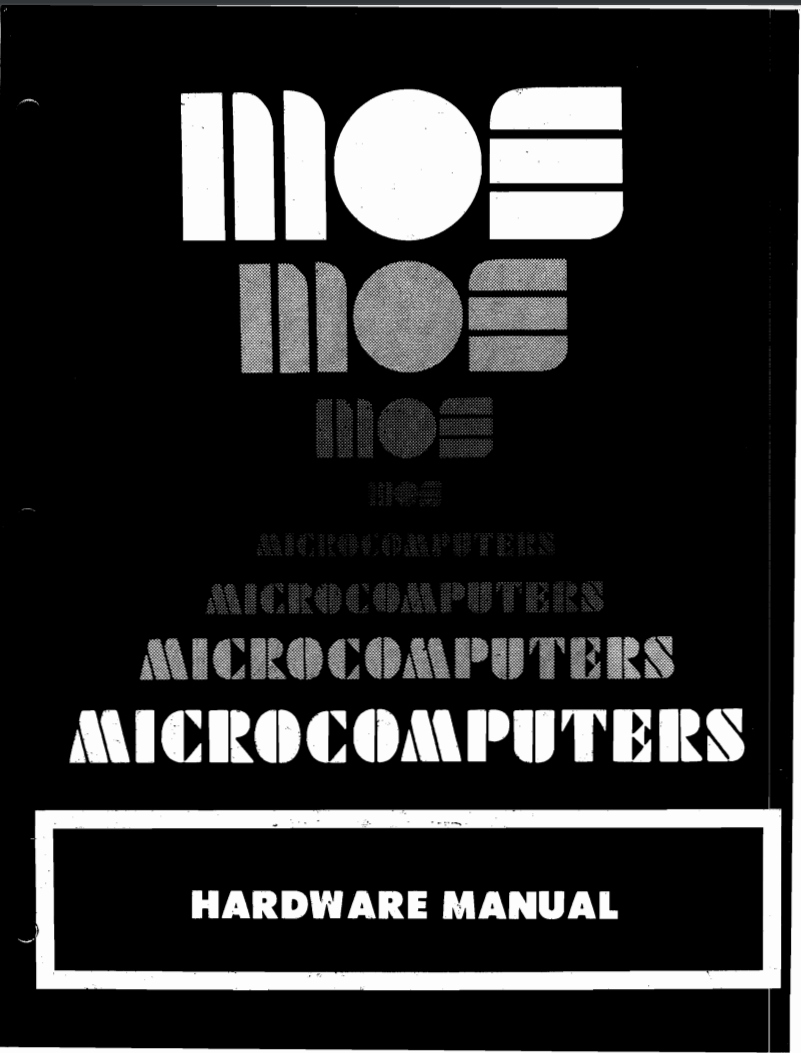
\includegraphics[width=0.25\textwidth]{images/mos-hw-manual.png}
	\caption{Obálka hardwarového manuálu rodiny komponent MCS6500 (sken archive.6502.org).}
	\label{fig:mos-hw-manual}
\end{figure}

\section{Nintendo Entertainment System}
Konzole Nintendo Entertainment System, často zkracována jako NES, je osmibitový zábavní počítačový systém firmy Nintendo, který byl vydán nejprve v Japonsku jako Family Computer (FC, \enquote{Famicom}). První verze je ukázaná na obrázku~\ref{fig:nes}. V~České republice je tento systém znám především díky mnoha klonům (\enquote{televizní hry na žlutých kazetkách}), které byly levnější a~dostupnější než oficiální systém. Tyto klony používaly kopie původního hardwaru, poté se objevily hardwarové emulátory založené na ASIC, které celou konzoli zmenšily do jednoho čipu (proto přezdívány NES-on-a-chip). Tato kapitola má za úkol popsat především technické specifikace systému --- zájemce o~podrobnou historii NES lze odkázat na Wikipedii~\cite{Wikipedia:NES}, \cite{Wikipedia:famiclone}, kde je mnoho odkazů na čínské klony konzole (často s~groteskními názvy: \enquote{Terminator 2 Super Design} od firmy \enquote{ENDING-MAN}, \enquote{Dr. Boy}, \enquote{Fun Time Home Computer: The New System}) a~článek~\cite{Svara:polystation}.

\begin{figure}[ht!]
	\centering
	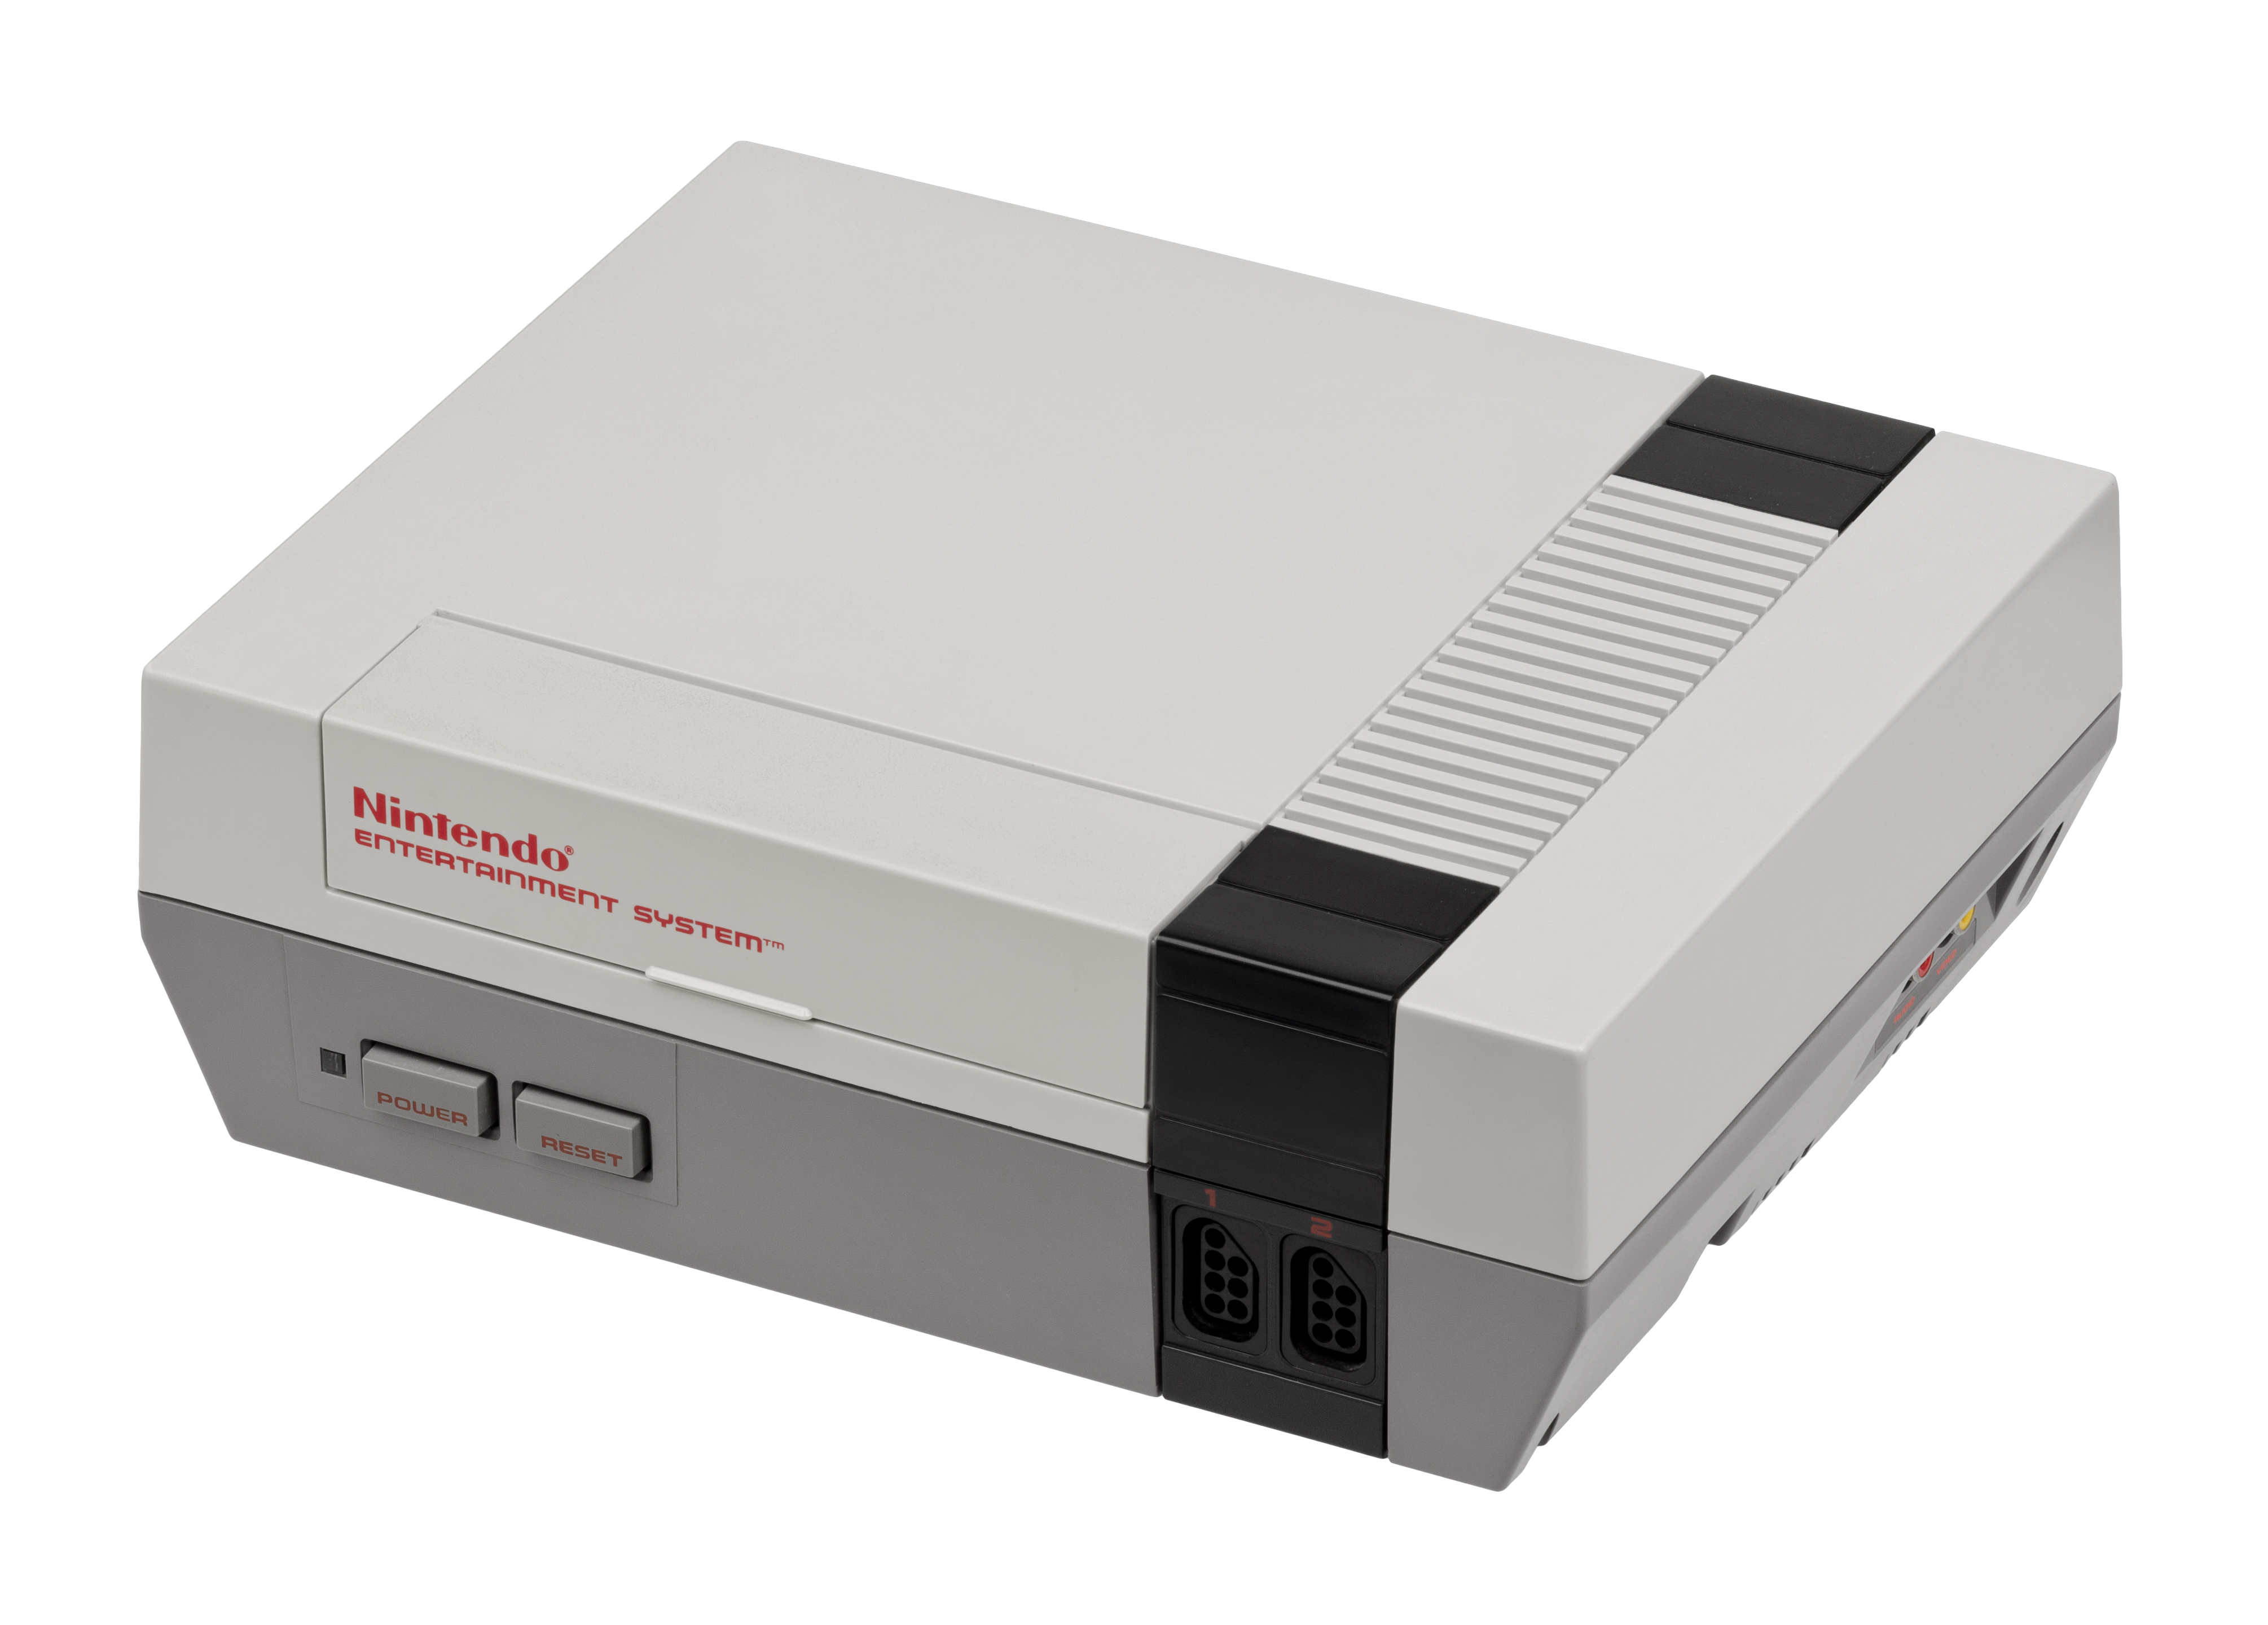
\includegraphics[width=0.4\textwidth]{images/nes.jpg}
	\caption{Konzole Nintendo Entertainment System (foto \copyright~2016, Evan-Amos).}
	\label{fig:nes}
\end{figure}


Systém se skládá z několika hlavních komponent, které spolu komunikují pomocí dvou sběrnic. Nejprve jsou představeny sběrnice a~k~nim připojené komponenty, jež jsou později popsány podrobněji.

\subsection{Hlavní sběrnice}
Hlavní sběrnice, kterou ilustruje obrázek~\ref{fig:nes-hlavnisbernice}, je adresována 16~bity a~přenáší 8~datových bitů. Komunikaci na hlavní sběrnici řídí pouze procesor~\emph{2A03}, který obsahuje i~řadič přímého přístupu do pamětí (DMA). Tudíž neexistuje (a~ani není potřebná) žádná forma arbitrace.

\begin{figure}[ht!]
	\centering
	% Kód pro renderování sběrnice byl inspirován příspěvkem od uživatele Ignasi na StackExchange.
	% https://tex.stackexchange.com/questions/319864/how-to-improve-my-draw-for-i2c-bus
	\begin{tikzpicture}[
		master/.style={draw, rounded corners, fill=mastercomponent, minimum height=15mm, minimum width=2.5cm},
		slave/.style={draw, rounded corners, fill=slavecomponent, minimum height=10mm, minimum width=2.5cm},
		slot/.style={draw, rounded corners, fill=interface, minimum height=10mm, minimum width=2.5cm}
		]
		
		\node[master] (m) {CPU (2A03)};
		\node[slave, below right=3mm and 7mm of m] (s1) {RAM};
		\node[slave, right= 3mm of s1] (s2) {APU};
		\node[slave, right= 3mm of s2] (s3) {PPU (2C02)};
		\node[slot, right= 3mm of s3] (s4) {I/O};
		
		\draw[thick] (m)--(m-|s4) node[above]{Hlavní sběrnice};
		\foreach \i in {1,2,3,4}{
			\draw[fill=black] (s\i)--(s\i|-m) circle (2pt);
		}
		
		\node[slave, below left=of s4] (gamepak) {Game Pak};	
		\draw[dashed] (s4)--(gamepak);
		
		
		\node[slave, below=of s4] (periferie) {Periferie};	
		\draw[dashed] (s4)--(periferie);
	\end{tikzpicture}
	\caption{Hlavní sběrnice konzole NES.}\label{fig:nes-hlavnisbernice}
\end{figure}

Procesor má k~dispozici 2~kB paměti RAM. Přímo v~procesoru se nachází čip pro generování zvuku, přezdívaný jako Audio Processing Unit (APU).  Na sběrnici se dále nachází grafický čip \emph{2C02}, označovaný jako Picture Processing Unit (PPU). Jako poslední je na sběrnici několik vstupně-výstupních (I/O) rozhraní: slot pro paměťové médium typu kazeta (cartridge), obchodně označovaná jako Game~Pak, pomocí níž se distribuoval veškerý software pro konzoli, a~porty pro periferie, především herní ovladače.

\begin{note}[APU a~hlavní sběrnice]
	APU, ačkoliv je součástí procesorového čipu, také komunikuje na hlavní sběrnici. Proto je na obrázku~\ref{fig:nes-hlavnisbernice} uveden jako další zařízení na sběrnici.
\end{note}

\subsection{Grafická sběrnice}
Systém obsahuje i~vedlejší sběrnici adresovanou 14~bity (celkem tedy 16~kB adresovatelného prostoru), kde komunikaci řídí PPU. Schematicky je znázorněna na obrázku~\ref{fig:nes-grafickasbernice}. Tato sběrnice je zcela oddělena od hlavní. Sběrnice obsahuje paměť video RAM (VRAM, také označována jako CIRAM) o~kapacitě 2~kB. Do paměťového prostoru je dále mapována RAM obsahující barevnou paletu. V~systému existuje ještě paměť OAM (Object Attribute Memory), která obsahuje seznam spritů a~informace potřebné k~jejich zobrazování. Ta ale není připojena ke sběrnici, nýbrž přímo k~čipu PPU.

\begin{definition}[Sprite]
	Sprite (počeštěně sprajt) je dvourozměrný obrázek, který bývá integrován do větších scén. Termín pochází z~dob, kdy se zvlášť vykreslovalo pozadí a~právě sprity, které často představovaly herní postavičky a~asociované předměty (zbraně, náboje a~další). To je případ i~konzole NES, která pro sprity měla dedikovanou paměť OAM.
\end{definition}

\begin{note}[Přístup CPU na grafickou sběrnici]
	Přestože není procesor přímo připojený na grafickou sběrnici, může na ní nepřímo komunikovat přes registry PPU (\$2006 a \$2007), které jsou mapovány na hlavní sběrnici (a~tím i~do adresního prostoru CPU). Tyto registry se používají i~pro přístup během DMA.
\end{note}

\begin{figure}[ht!]
	\centering
	% Kód pro renderování sběrnice byl inspirován příspěvkem od uživatele Ignasi na StackExchange.
	% https://tex.stackexchange.com/questions/319864/how-to-improve-my-draw-for-i2c-bus
	\begin{tikzpicture}[
		master/.style={draw, rounded corners, fill=mastercomponent, minimum height=15mm, minimum width=2.5cm},
		slave/.style={draw, rounded corners, fill=slavecomponent, minimum height=10mm, minimum width=2.5cm},
		slot/.style={draw, rounded corners, fill=interface, minimum height=10mm, minimum width=2.5cm}
		]
		
		\node[master] (m) {PPU (2C02)};
		\node[slave, below right=3mm and 7mm of m] (s1) {VRAM};
		\node[slave, right= 6mm of s1] (s2) {Paletová RAM};
		\node[slave, below=of m] (s3) {OAM};
		
		\draw[thick] (m)--(m-|s2.east) node[above]{Grafická sběrnice};
		\foreach \i in {1,2}{
			\draw[fill=black] (s\i)--(s\i|-m) circle (2pt);
		}
		\draw[dashed] (m) -- (s3);
		
	\end{tikzpicture}
	\caption{Grafická sběrnice konzole NES.}\label{fig:nes-grafickasbernice}
\end{figure}

\section{Procesor 6502}
Základem NES je klon procesoru \emph{6502}, označený jako \emph{2A03}. Tato podkapitola popisuje původní variantu procesoru a~specifika klonu jsou popsány v~samostatné podkapitole~\ref{sec:2A03}.

\subsection{Historie}
Procesor 6502 navrhla firma MOS Technology v~roce 1975. Na procesoru pracoval tým, který původně navrhoval mikroprocesor Motorola 6800. Čip 6502 vznikl jako levnější a~rychlejší alternativa procesoru od Motoroly pod vedením Chucka Peddla~\cite{computer-history-museum:chuck-peddle}, která zachovává hardwarovou kompatibilitu. Cílem bylo umožnit využití i~v~projektech, kde by jinak byla levnější diskrétní logika~\cite{mos:hw-manual}. Ve své podstatě jde o~aplikaci programovatelného počítače (definovaného v~kapitole~\ref{chap:predstaveni-problematiky}) v~praxi --- funkce zařízení lze změnit pouze výměnou programu, což byl i~jediný požadavek při přechodu z~konkurenční Motoroly; upravit program pro ISA 6502.

\subsection{Interakce procesoru s~prostředím}
Na úvod, jak se píše v~hardwarovém manuálu~\cite{mos:hw-manual}, je vhodné se zabývat tím, v~jakém prostředí procesor bude pracovat~a jak s~ním bude interagovat. Prostředím je myšlen systém, který bude procesorem řízen. Procesor 6502 s okolím komunikuje pomocí jedné systémové sběrnice, která obsahuje 16~adresních vodičů, 8~datových vodičů a~signál R/W, který signalizuje zdroj dat vzhledem k~procesoru. Logická jednička (napětí větší než 2,4~V) signalizuje čtení procesorem, logická nula pak zápis procesorem. Okolí procesoru je tvořeno několika komponentami, ty jsou součástí adresního prostoru CPU, který je znázorněn v~tabulce~\ref{tab:cpu-adresniprostor}.

Adresní prostor je v~terminologii produktové řady MCS650X rozdělen na stránky, což představuje rozsah adresovatelný jedním bajtem (256 adres). Index v~rámci stránky zajišťuje spodní bajt, index stránky poté horní bajt. Z~toho vyplývá, že stránek je také 256. Znalost tohoto faktu je klíčová pro pochopení důvodu existence speciálního zero-page adresního režimu, který je vysvětlen v~podkapitole~\ref{sec:6502-adresni-rezimy}.

\begin{table}[ht!]
	\centering
	\caption{Adresní prostor CPU.}\label{tab:cpu-adresniprostor}
	\begin{tblr}{|Q[c,m]|Q[c,m]|}
		\hline
		Adresní rozsah & Zařízení \\
		\hline[2pt]
		\$0000–\$07FF & RAM \\
		\hline
		\$0800–\$1FFF & Zrcadlo \$0000–\$07FF \\
		\hline
		\$2000–\$2007 & Registry PPU \\
		\hline
		\$2008–\$3FFF & Zrcadlo \$2000–\$2007 \\
		\hline
		\$4000–\$4017 & Registry APU a I/O \\
		\hline
		\$4018–\$401F & Nepoužíváno \\
		\hline
		\$4020–\$FFFF & Game Pak \\
		\hline
	\end{tblr}
\end{table}

Komunikace je řízena dvoufázovými systémovými hodinami. V~první fázi se vystaví adresa na sběrnici (předstih), v~druhé fázi dochází k~přenosu dat. Z~těchto dvou fází se pak skládá celý procesorový cyklus~\cite{mos:hw-manual}. Příklad komunikace směrem k~procesoru (čtení) je znázorněn na obrázku~\ref{fig:6502-casovani-cteni}. Dle dokumentace je pro 1MHz hodiny garantováno, že adresa bude stabilní 300~ns po náběžné hraně první fáze; naopak je požadováno, aby data byla platná alespoň 100~ns před sestupnou hranou druhé fáze hodin.

\begin{figure}[ht!]
	\centering
	\begin{tikztimingtable}[%
		timing/dslope=0.1,
		timing/.style={x=5ex,y=3ex},
		x=5ex,
		timing/rowdist=4ex,
		timing/name/.style={font=\sffamily\scriptsize}
		]
		\signal{CLK $\phi1$}     & L l H H H L L L h \\
		\signal{CLK $\phi2$}     & H L L L H H H L  \\
		\signal*{R/W}            & L l h 6H \\
		\signal[15:0]{ADRESA}    & 1.5D{...} U 4.5D{adresa do paměti} U \\
		\signal[7:0]{DATA}       & 5.5Z 2D{data z paměti} u  \\
		\extracode
		\begin{pgfonlayer}{background}
			\begin{scope}[semitransparent ,semithick]
				\vertlines[black,dotted]{1.0,2.0,...,7.5}
				\vertlines[gray,dotted]{0.5,1.5,...,8.0}
			\end{scope}
		\end{pgfonlayer}
	\end{tikztimingtable}
	\caption{Časování čtení procesoru.}\label{fig:6502-casovani-cteni}
\end{figure}

Kromě systémové sběrnice existuje další způsob komunikace, a~to je přerušení. Všechny procesory v~produktové řadě MCS650X obsahují celkem tři vstupy reprezentující různá přerušení: RST, IRQ a~NMI.

\subsection{Architektura}
Po diskusi vnější komunikace procesoru je vhodné se zabývat jeho architekturou, a~nejen instrukční sadou, ale i~implementačními detaily tam, kde je to nutné. Architekturou se zabývá především softwarový manuál~\cite{mos:sw-manual}.

Procesor 6502 je osmibitový, jelikož pracuje se slovem o~velikosti osmi bitů. ISA procesoru 6502 je střadačově orientovaná, pracovní registr je totiž právě pouze střadač (akumulátor). ISA definuje adresu jako 16bitové číslo ve formátu little-endian, jako první je tedy vždy uváděn nejméně významný bajt (LSB). ISA také definuje několik adresních režimů, z~toho jeden speciální, zero-page režim, který slouží jako částečná náhrada absence více registrů a~efektivně činí z~první paměťové stránky pomyslnou zápisníkovou paměť.

Nejprve je potřeba analyzovat datovou cestu pro pochopení, jaký hardware mají jednotlivé instrukce k~dispozici. Dále adresní režimy, jelikož struktura a~délka instrukcí a~instrukční cyklus s~nimi pevně souvisí.

\begin{note}[Značení adresních bajtů]
	Jelikož je adresa uváděna po bajtech a~obsahuje právě dva bajty, bylo zavedeno v~rámci příruček firmy MOS označení ADL (address low) pro nejméně významný (nižší) bajt adresy a~ADH (address high) pro nejvíce významný (vyšší) bajt. Tohoto značení se drží i~bakalářská práce.
\end{note}

\subsubsection{Datová cesta}
Procesor 6502 obsahuje ve své datové cestě několik registrů. V~tabulce~\ref{tab:6502-registry} je uveden popis registrů s~velikostmi, často používanými zkratkami a~popisem obsahu.

\begin{table}[ht!]
	\centering
	\caption{Registry procesoru 6502.}\label{tab:6502-registry}
	\begin{tblr}{|Q[c,m]|Q[c,m]|Q[c,m]|X[c,m]|}
		\hline
		Registr & Zkratka & Velikost (bit) & Obsah \\
		\hline[2pt]
		programový čítač & PC & 16 & adresa instrukce ke zpracování \\
		\hline
		střadač (akumulátor) & A & 8 & zpracovávané hodnoty \\
		\hline
		ukazatel zásobníku & S & 8 & adresa vrcholu zásobníku \\
		\hline
		indexovací registr X & X & 8 & adresní offset \\
		\hline
		indexovací registr Y & Y & 8 & adresní offset \\
		\hline
		registr příznaků & P & 8 & výsledky provedení ALU operací a~stav CPU \\ 
		\hline
	\end{tblr}
\end{table}

Střadač v ISA 6502 má podobný účel jako v~jiné střadačové architektuře. Jedná se o~jediný univerzální registr, kde všechny operace (kromě načítání a~ukládání, což zvládají i~indexovací registry) musí být prováděny přes zásobník. Střadač je implicitním úložným místem pro výsledky operací.

Zásobník architektury 6502 je fixován na adresách \$0100--\$01FF. Jeho kapacita je tedy 256 bajtů a~roste odshora dolů. Se zásobníkem se manipuluje pomocí dedikovaných instrukcí, je možné na zásobník uložit střadač nebo obsah příznakového registru. Adresa vrcholu zásobníku je v~registru S. 

Indexovací registry slouží primárně jako zdroj offsetu pro adresní režimy s~indexací. Fungují jako čítač, existují instrukce pro jejich inkrementaci (INX, INY), dekrementaci (DEX, DEY) a~porovnávání hodnot s~hodnotou v~paměti (CPX, CPY). Jelikož se ale jejich hodnota načítá z~paměti a~lze do paměti i~uložit, mohou sloužit jako programem využitelné pomocné registry.

Příznakový registr obsahuje 7 využívaných příznaků. Jejich popis je v~tabulce~\ref{tab:6502-flags}. Index označuje pořadí bitu (zprava), do kterého se daný příznak ukládá při použití instrukce PHP. Příznakem, který ve fyzickém registru není implementován, je B. Tento příznak je viditelný pouze při operaci přenosu registru příznaků do zásobníku a~jeho hodnota záleží na tom, která operace přenos do zásobníku vyvolala. Přenos je vyvolán dvěma způsoby:

\begin{itemize}
	\item softwarově (instrukce BRK a~PHP): hodnota B je 1,
	\item hardwarově (přerušení): hodnota B je 0.
\end{itemize}

Tím, že registr B nemá hardwarovou reprezentaci, je jeho hodnota ignorována při navrácení příznaků ze zásobníků.

\begin{table}[ht!]
		\centering
		\caption{Popis příznakového registru procesoru 6502.}\label{tab:6502-flags}
		\begin{tblr}{|Q[c,m]|Q[c,m]|X[c,m]|}
			\hline
			Index & Příznak &  Popis \\
			\hline[2pt]
			0 & C & Operace vygenerovala přenos. \\
			\hline
			1 & Z & Zpracovávaná hodnota je nulová. \\
			\hline
			2 & I  & Maska přerušení (hodnota 1: přerušení maskováno) . \\
			\hline
			3 & D & Režim BCD (hodnota 1: režim je aktivní). \\
			\hline
			4 & B & Příznak \enquote{break}. Neexistuje fyzicky. \\
			\hline
			5 & - & Nepoužito. \\
			\hline
			6 & V & Operace vyvolala přetečení. \\
			\hline
			7 & N & Zpracovávaná hodnota je záporná (má-li sedmý bit má hodnotu 1) \\
			\hline
		\end{tblr}
	\end{table}

Procesor dále obsahuje pomocné registry pro dočasné ukládání paměti a~dat (programově nepřístupné; používané při přístupu na sběrnici). Nedílnou součástí je pak také aritmeticko-logická jednotka, ve které probíhají nejen konkrétní výpočty požadované instrukcemi, ale i~pomocné výpočty například pro zjištění absolutní adresy při vyhodnocování skoků.

\subsubsection{Základní adresní režimy}
\label{sec:6502-adresni-rezimy}
Základní adresní režimy pracují pouze s~pevnými adresními hodnotami. Patří mezi ně implikovaný režim, okamžitý režim, absolutní režim, režim nulté stránky a~relativní režim.

Nejjednodušší adresní režim se skládá pouze z~operačního znaku (OZ, anglicky opcode), který jednoznačně identifikuje příslušnou instrukci. Sama instrukce implikuje, s~jakými daty se bude pracovat, proto je tento režim nazván \emph{implikovaný} a~taková instrukce má vždy 1 bajt. Struktura a~příklad instrukce je znázorněn na obrázku~\ref{fig:6502-adr-impl}.

\begin{figure}[ht!]
	\centering
	\begin{bytefield}[bitheight=\widthof{~Sign~},
		boxformatting={\centering\small\ttfamily}]{8}
		\bitbox[]{8}{}    		   & \bitheader[endianness=little]{0,7} \\
		\bitbox[]{8}{}    		   & \bitbox{8}[bgcolor=bfcommon]{OZ} \\
		\bitbox[]{8}{}    		   & \bitheader[endianness=little]{0,7} \\
		\bitbox[]{8}{CLI} & \bitboxes*{1}[bgcolor=bfcommonlight]{01011000}
	\end{bytefield}
	\caption{Struktura instrukce implikovaného adresního režimu s~příkladem instrukce Clear Interrupt Disable Bit (CLI).}\label{fig:6502-adr-impl}
\end{figure}

Další adresní režim pracuje s~konstantní hodnotou, která je uváděná ihned za operačním znakem. To znamená, že se zpracovávaná hodnota nemusí načítat z~paměti pomocí adresy, ale nachází se přímo ve zpracovávaném kódu. Označuje se jako \emph{okamžitý} (immediate) a~instrukci tak tvoří dva bajty. Příklad je uveden na obrázku~\ref{fig:6502-adr-imm}; instrukce AND provede logický součin hodnoty v~akumulátoru s~konstantou \$42.

\begin{figure}[ht!]
	\centering
	\begin{bytefield}[bitheight=\widthof{~Sign~},
		boxformatting={\centering\small\ttfamily}]{8}
		\bitbox[]{8}{}    		   & \bitheader[endianness=little]{0,7,8,15} \\
		\bitbox[]{8}{}    		   & \bitbox{8}[bgcolor=bfcommon]{OZ} & \bitbox{8}[bgcolor=bfcommon]{konstanta} \\
		\bitbox[]{8}{}    		   & \bitheader[endianness=little]{0,7,8,15} \\
		\bitbox[]{8}{AND} & \bitboxes*{1}[bgcolor=bfcommonlight]{00101001} & \bitboxes*{1}[bgcolor=bfcommonlight]{01000010}
	\end{bytefield}
	\caption{Struktura instrukce okamžitého adresního režimu s~příkladem instrukce AND Memory with Accumulator (AND).}\label{fig:6502-adr-imm}
\end{figure}

Adresní režim, který již pracuje s~hodnotami adres, se označuje jako \emph{absolutní}. Součástí instrukce v~tomto režimu je přímá hodnota adresy, kde se nachází kýžená data. Instrukce je tedy 3 bajtová. Formát instrukce i~s~příkladem je na obrázku~\ref{fig:6502-adr-abs}; demonstrovaná instrukce načte do akumulátoru hodnotu ze~zařízení v~adresním prostoru procesoru na adrese \$102.

\begin{figure}[ht!]
	\centering
	\begin{bytefield}[bitheight=\widthof{~Sign~},
		boxformatting={\centering\small\ttfamily}]{8}
		\bitbox[]{8}{}    		   & \bitheader[endianness=little]{0,7,8,15,16,23} \\
		\bitbox[]{8}{}    		   & \bitbox{8}[bgcolor=bfcommon]{OZ} & \bitbox{8}[bgcolor=bfcommon]{ADL} & \bitbox{8}[bgcolor=bfcommon]{ADH} \\
		\bitbox[]{8}{}    		   & \bitheader[endianness=little]{0,7,8,15,16,23}  \\
		\bitbox[]{8}{LDA} & \bitboxes*{1}[bgcolor=bfcommonlight]{10101101} & \bitboxes*{1}[bgcolor=bfcommonlight]{00000010} & \bitboxes*{1}[bgcolor=bfcommonlight]{00000001}
	\end{bytefield}
	\caption{Struktura instrukce absolutního adresního režimu s~příkladem instrukce Load Accumulator (LDA).}\label{fig:6502-adr-abs}
\end{figure}

Absence univerzálních registrů je částečně suplována existencí adresního režimu \emph{nulté stránky} (zero-page). Adresa, která je uvedena za OZ, je jednobajtová. V~tomto režimu je možné indexovat pouze v~rámci jedné stránky, a~to té první (při indexování od nuly nulté) (adresní rozsah \$0000--\$00FF). Zato však tyto instrukce zabírají dva bajty v~instrukční paměti a~jejich zpracování je rychlejší. Na nultou paměťovou stránku je tak možné nahlížet jako na formu ručně spravované cache~---~v~programátorském manuálu řady MSC6500~\cite{mos:sw-manual} je zdůrazněno, že je program možné optimalizovat přesunem nejčastěji používaných hodnot právě do nulté stránky. Formát je znázorněn na obrázku~\ref{fig:6502-adr-zp}; instrukce Store Accumulator načte do akumulátoru bajt z~první paměťové stránky s offsetem \$42.

\begin{figure}[ht!]
	\centering
	\begin{bytefield}[bitheight=\widthof{~Sign~},
		boxformatting={\centering\small\ttfamily}]{8}
		\bitbox[]{8}{}    		   & \bitheader[endianness=little]{0,7,8,15} \\
		\bitbox[]{8}{}    		   & \bitbox{8}[bgcolor=bfcommon]{OZ} & \bitbox{8}[bgcolor=bfcommon]{ADL} \\
		\bitbox[]{8}{}    		   & \bitheader[endianness=little]{0,7,8,15}  \\
		\bitbox[]{8}{STA} & \bitboxes*{1}[bgcolor=bfcommonlight]{10000101} & \bitboxes*{1}[bgcolor=bfcommonlight]{01000010}
	\end{bytefield}
	\caption{Struktura instrukce adresního režimu nulté stránky s~příkladem instrukce Store Accumulator (STA).}\label{fig:6502-adr-zp}
\end{figure}

\emph{Relativní} adresování je používáno výlučně instrukcemi větvení. Obsahuje pouze jeden adresní bajt, který reprezentuje offset v~dvojkovém doplňku. Vyhodnotí-li se podmínka skoku kladně a~skok se tedy provádí, je hodnota offsetu přičítána k~adrese následující instrukce (než se podmínka skoku vyhodnotí, nachází se již programový čítač na další adrese). V~JSA obecně není nutné uvádět offset explicitně, uvádí se konkrétní adresa, nebo návěští; pomocí těchto údajů je assembler schopen výsledný offset dopočítat. Režim je demonstrován na instrukci Branch~On~Carry~Set na obrázku~\ref{fig:6502-adr-rel} s~offsetem \$42.

\begin{figure}[ht!]
	\centering
	\begin{bytefield}[bitheight=\widthof{~Sign~},
		boxformatting={\centering\small\ttfamily}]{8}
		\bitbox[]{8}{}    		   & \bitheader[endianness=little]{0,7,8,15} \\
		\bitbox[]{8}{}    		   & \bitbox{8}[bgcolor=bfcommon]{OZ} & \bitbox{8}[bgcolor=bfcommon]{offset} \\
		\bitbox[]{8}{}    		   & \bitheader[endianness=little]{0,7,8,15}  \\
		\bitbox[]{8}{BCS} & \bitboxes*{1}[bgcolor=bfcommonlight]{10110000} & \bitboxes*{1}[bgcolor=bfcommonlight]{01000010}
	\end{bytefield}
	\caption{Struktura instrukce relativního adresování s~příkladem instrukce Branch On Carry Set (BCS).}\label{fig:6502-adr-rel}
\end{figure}

\subsubsection{Adresní režimy s~indexací}
Složitější adresní režimy přinášejí další možnosti přístupu k~datům v~paměti. Do této chvíle byly uvedeny pouze takové režimy, které disponují pouze pevně stanovenou adresou. Často je však nutné adresy měnit, nebo vytvářet zcela dynamicky. Takový typ adres označuje manuál~\cite{mos:sw-manual} jako počítané adresy. Pro práci s~počítanými adresami obsahuje ISA speciální adresní režimy využívající indexovací registry: absolutní režim s~indexací a~režim nulté stránky s~indexací.

\begin{example}[Kopírování souvislých dat bez indexace]
Jedním ze základních řídicích struktur programovacích jazyků jsou cykly, které mohou posloužit jako nástroj pro práci s~bloky dat. Typickým příkladem nechť je kopírování dat z~jednoho paměťového místa na jiné. Ve střadačové architektuře se provádí načtením do střadače a~uložením.

Byla-li by implementace provedena pouze za použití pevných adres, musela by se pro každé paměťové místo uvést instrukce načtení i~instrukce zápisu. Vytváří-li se adresy dynamicky, je možné provést operace v~cyklu. Ačkoliv existuje způsob úpravy pevných adres za běhu programu pomocí techniky samomodifikujícího se kódu (viz stranu 72 manuálu~\normalfont{\cite{mos:sw-manual}}), představují adresní režimy s~indexací elegantnější alternativu nevyžadující přepisovatelnou instrukční paměť.
\end{example}

Nechť je jako první uveden \emph{absolutní adresní režim s~indexací}. Tento režim přidává absolutnímu režimu možnost přičíst k~původní adrese i~offset z~registru X, nebo Y; dle zvoleného registru se tak jedná o~dva různé adresní režimy. Adresa pevně určená instrukcí je nazývaná jako základová (base). Výsledná adresa je vypočtena jednoduše součtem základové adresy a~offsetu. Struktura je stejná jako u standardního absolutního režimu na obrázku~\ref{fig:6502-adr-abs}.

Podobně jako u~standardních režimů existuje možnost pracovat pouze s~nultou stránkou. K~tomu~účelu slouží \emph{režim nulté stránky s~indexací}. Struktura instrukce je opět stejná jako na obrázku~\ref{fig:6502-adr-zp}. V~tomto režimu nedochází k~překročení paměťových stránek při přičtení indexu, horní bajt je ignorován a~výpočty tak efektivně probíhají v~modulu \$100. Výpočet tedy probíhá jako: $(\textrm{zakladova\_adresa} + \textrm{offset}) \mod 256$. Kromě instrukcí LDX a~STX, kdy jsou k~dispozici oba indexovací registry k~výběru, je tento režim použitelný pouze s~registrem X.

\subsubsection{Nepřímé adresování}
V~architektuře 6502 existuje ještě \emph{nepřímé adresování}, které umožňuje pracovat s~ukazateli namísto s~přímou hodnotou adresy. Takové režimy jsou dva, indexovaný-nepřímý a nepřímý-indexovaný. Názvy režimů jsou odvozené podle pořadí, ve kterém se přičítá index.

První zmíněný režim, \emph{indexovaný-nepřímý}, pracuje s~jednobajtovou adresou následovanou po operačním znaku. Tato adresa je základ ukazatele do nulté stránky. K~základu se přičte hodnota indexovacího registru X. Součet probíhá opět v modulu 256, vyšší bajt je totiž zahazován. Vznikne tak výsledný ukazatel, který směřuje na místo nacházející se v~nulté stránce, které obsahuje první bajt kýžené adresy. Ta je opět uspořádána ve formátu nižší bajt a~vyšší bajt. Příklad na obrázku~\ref{fig:6502-adr-idx-ind} ukazuje variantu instrukce STA v~indexovaném-nepřímém režimu. Samotný OZ se základem ukazatele je umístěn v~instrukční pamětí na adrese \$F000. K~základu \$42 je přičten obsah registru X \$10. Výsledkem je adresa \$52, na které se již nachází 16bitová konečná adresa. Instrukce STA v~popsaném příkladě tedy uloží hodnotu akumulátoru až na adresu zjištěnou v~posledním kroku: \$3412.

\begin{figure}[ht!]
	\centering
	\begin{bytefield}[bitheight=\widthof{~Sign~},
		boxformatting={\centering\small\ttfamily}]{8}
		\bitbox[]{8}{} & \bitheader[endianness=little]{0,7,8,15} \\
		\bitbox[]{8}{\$F000:} & \bitbox{8}[bgcolor=bfcommon]{OZ} & \bitbox{8}[bgcolor=bfcommon]{základ ukazatele} & \bitbox[]{8}{} & \bitbox{8}[bgcolor=bfaux]{X} \\

		\bitbox[]{8}{} & \bitboxes*{1}[bgcolor=bfcommonlight]{10000001} & \bitbox{8}[bgcolor=bfcommonlight]{\$42} & \bitbox[]{8}{} & \bitbox{8}[bgcolor=bfauxlight]{\$10} \\ \\ \\

		\bitbox[]{8}{Výpočet:} & \bitbox{8}[bgcolor=bfcommonlight]{\$42} & \bitbox{1}[]{+} & \bitbox{8}[bgcolor=bfauxlight]{\$10} \\

		\bitbox[]{8}{} & \bitheader[endianness=little]{0,7,8,15} \\ \bitbox[]{8}{\$52:} & \bitbox{8}[bgcolor=bfcommon]{ADL} & \bitbox{8}[bgcolor=bfcommon]{ADH} \\
		
		\bitbox[]{8}{} & \bitbox{8}[bgcolor=bfcommonlight]{\$12} & \bitbox{8}[bgcolor=bfcommonlight]{\$34}
	\end{bytefield}
	\caption{Struktura instrukce indexovaného-nepřímého režimu s~příkladem instrukce STA.}\label{fig:6502-adr-idx-ind}
\end{figure}

Druhý režim, \emph{nepřímý-indexovaný}, funguje podobně, ale přičítání indexu probíhá až v~druhém kroku a~používá se registr Y. Po operačním znaku následuje hodnota ukazatele, která se již nemění. Ukazuje do nulté stránky, kde se nachází dvojbajtový základ konečné adresy. K~základu se přičte hodnota registru Y. Vznikne tak konečná adresa, se kterou může daná instrukce dále pracovat. Příklad opět na instrukci STA je uveden na obrázku~\ref{fig:6502-adr-ind-idx}. Tentokrát bude hodnota akumulátoru uložena na adresu \$3422.

\begin{figure}[ht!]
	\centering
	\begin{bytefield}[bitheight=\widthof{~Sign~},
		boxformatting={\centering\small\ttfamily}]{8}
		\bitbox[]{8}{} & \bitheader[endianness=little]{0,7,8,15} \\
		\bitbox[]{8}{\$F000:} & \bitbox{8}[bgcolor=bfcommon]{OZ} & \bitbox{8}[bgcolor=bfcommon]{ukazatel} & \bitbox[]{8}{} & \bitbox{8}[bgcolor=bfaux]{X} \\
		
		\bitbox[]{8}{} & \bitboxes*{1}[bgcolor=bfcommonlight]{10000001} & \bitbox{8}[bgcolor=bfcommonlight]{\$42} & \bitbox[]{8}{} & \bitbox{8}[bgcolor=bfauxlight]{\$10} \\
		
		\bitbox[]{8}{} & \bitheader[endianness=little]{0,7,8,15} \\ \bitbox[]{8}{\$42:} & \bitbox{8}[bgcolor=bfcommon]{ADL} & \bitbox{8}[bgcolor=bfcommon]{ADH} \\
		
		\bitbox[]{8}{} & \bitbox{8}[bgcolor=bfcommonlight]{\$12} & \bitbox{8}[bgcolor=bfcommonlight]{\$34} \\ \\ \\
		
		\bitbox[]{8}{Výpočet:} & \bitbox{8}[bgcolor=bfcommonlight]{\$3412} & \bitbox{1}[]{+} & \bitbox{8}[bgcolor=bfauxlight]{\$10} \\
	\end{bytefield}
	\caption{Struktura instrukce nepřímého-indexovaného režimu s~příkladem instrukce STA.}\label{fig:6502-adr-ind-idx}
\end{figure}

Existuje ještě jeden nepřímý režim, označovaný jako \emph{nepřímý absolutní}. Tento režim je použit pouze instrukcí skoku (JMP). Princip je podobný jako u~zmíněných nepřímých režimů s~tím rozdílem, že nedochází k~přičítání indexu. Instrukce se skládá z~operačního znaku a~dvou adresních bajtů, které fungují jako 16bitový ukazatel na výslednou adresu, na kterou se má skočit. V~příkladu na obrázku~\ref{fig:6502-adr-ind} instrukce JMP skočí na adresu uloženou na adrese \$2010, jejíž hodnota je \$FA55 --- skok bude tedy proveden na adresu \$FA55.

\begin{figure}[ht!]
	\centering
	\begin{bytefield}[bitheight=\widthof{~Sign~},
		boxformatting={\centering\small\ttfamily}]{8}
		\bitbox[]{8}{} & \bitheader[endianness=little]{0,7,8,15,16,23} \\
		\bitbox[]{8}{\$F000:} & \bitbox{8}[bgcolor=bfcommon]{OZ} & \bitbox{8}[bgcolor=bfcommon]{ukazatel (LO)} & \bitbox{8}[bgcolor=bfcommon]{ukazatel (HI)} \\
		
		\bitbox[]{8}{} & \bitboxes*{1}[bgcolor=bfcommonlight]{01101100} & \bitbox{8}[bgcolor=bfcommonlight]{\$10} & \bitbox{8}[bgcolor=bfcommonlight]{\$20} \\
		
		\bitbox[]{8}{} & \bitheader[endianness=little]{0,7,8,15} \\ \bitbox[]{8}{\$2010:} & \bitbox{8}[bgcolor=bfcommon]{ADL} & \bitbox{8}[bgcolor=bfcommon]{ADH} \\
		
		\bitbox[]{8}{} & \bitbox{8}[bgcolor=bfcommonlight]{\$55} & \bitbox{8}[bgcolor=bfcommonlight]{\$FA} \\
	\end{bytefield}
	\caption{Struktura instrukce JMP využívající nepřímý absolutní adresní režim s~příkladem skoku na adresu \$FA55.}\label{fig:6502-adr-ind}
\end{figure}

\begin{example}[Využití nepřímého adresování]
Nepřímé adresování má mnoho různých využití. U indexovaného-nepřímého se jedná především o~práci se seznamem adres. Tento seznam může uchovávat například adresy tlačítek herních ovladačů, ze kterých se periodicky vyčítá stav. Nepřímý-indexovaný pak může sloužit k~modifikaci chování volaného podprogramu. Úpravou hodnoty registru Y bude podprogram pracovat s~jiným offsetem v~odkazované paměti.
\end{example}

\subsubsection{Instrukční cyklus}
\label{sec:6502-instrukcni-cyklus}
Instrukční cyklus odpovídá standardnímu cyklu procesoru, jako uvádí prof. Kubátová v~\cite{Kubatova2018:SAP}; fetch (načtení instrukce), decode (dekódování instrukce), execute (provedení instrukce). Dekódování je věnována zvláštní pozornost v~podkapitole~\ref{sec:6502-dekodovani-instrukci}. Standardně je součástí běhu navíc počáteční nastavení při spuštění a~ošetření příčiny přerušení; právě tomuto je věnována zvláštní pozornost v~podkapitolách~\ref{sec:6502-reset} a~\ref{sec:6502-preruseni}.

\begin{figure}[ht!]
	\centering
	\begin{tikzpicture}[node distance=2cm] 
		\tikzstyle{akce} = [rectangle, minimum width=4cm, minimum height=1cm, text centered, draw=black, fill=fcaction]
		\tikzstyle{startstop} = [rectangle, rounded corners, minimum width=3cm, minimum height=1cm,text centered, draw=black, fill=fcstart]
		\tikzstyle{vetveni} = [diamond, minimum width=3cm, minimum height=1cm, text centered, draw=black, fill=fcbranch]
		\tikzstyle{arrow} = [thick,->,>=stealth]
		
		\node (start) [startstop] {Start};
		\node (IC) [vetveni, below of=start] {Přerušení?};
		\node (IS) [akce, right of=IC, xshift=3cm] {Obsluha přerušení};
		\node (IF) [akce, below of=IC] {Načtení instrukce};
		\node (ID) [akce, below of=IF] {Dekódování instrukce};
		\node (EX) [akce, below of=ID] {Provedení instrukce};
		\node (aux) [left=2cm of IC] {};
		
		\draw [arrow] (start) -- (IC);
		\draw [arrow] (IC) -- node[anchor=south] {ano} (IS);
		\draw [arrow, <-] (IF) -| (IS);
		\draw [arrow] (IC) -- node[anchor=east] {ne} (IF);
		\draw [arrow] (IF) -- (ID);
		\draw [arrow] (ID) -- (EX);
		\draw [arrow] (EX) -| (aux);
		\draw [arrow] (aux) -- (IC);
	\end{tikzpicture} 
	\caption{Instrukční cyklus procesoru.}\label{fig:6502-instrukcni-cyklus}
\end{figure}

Přesné dodržení instrukčního cyklu nemusí být u~emulace nutné, dokonce bývá zvykem velkou část cyklu zjednodušit pro dosažení většího výkonu tak, že se pracuje pouze na úrovni instrukcí. Jelikož je ale v~systému komponent více, je nutné se zabývat alespoň délkou trvání jednotlivých instrukcí, aby nedocházelo ke ztrátě synchronizace. 

Délka zpracování instrukce je vázána především na její typ a podtyp --- pohybuje se od 2 do 7 (8 v~případě nedokumentovaných instrukcí) strojových cyklů. Instrukce totiž existují ve více variantách v~závislosti na použitém adresním režimu. Každý podtyp je jednoznačně identifikován operačním znakem. To znamená, že pro stejnou instrukci existuje více různých operačních znaků, lišících se pouze v~adresním režimu. Je tedy možné délku zpracování odvodit pouze na základě operačního znaku.

Existují však výjimky. U~některých instrukcí pracujících s~pamětí může dojít k~překročení paměťové stránky, což způsobí provedení jednoho strojového cyklu navíc. To se týká adresních režimů pracujících s~indexy, konkrétně absolutního režimu s~indexací pro registry X i~Y. Týká se to i~nepřímého-indexovaného režimu, ten totiž také přičítá hodnotu registru k~16bitové adrese s~možností překročení stránky. Indexovaný-nepřímý režim již nedovoluje překročení paměťové stránky (horní bajt je vždy ignorován a~k~přenosu do vyššího řádu tak nedochází); jej se to již tedy netýká.

Poslední výjimkou jsou instrukce větvení. Dojde-li ke kladnému vyhodnocení podmínky, musí se vykonat jeden strojový cyklus navíc; to je způsobeno nutností přičíst offset k~programovému čítači. Dojde-li navíc k~překročení paměťové stránky, musí se kvůli přičtení přenosu provést ještě další strojový cyklus. Abych to shrnul, je-li proveden skok, který navíc překračuje stránku, provedou se navíc celkem dva strojové cykly.

\begin{note}[6502 a pipelining]
	Procesor 6502 zároveň provádí více činností --- operace na vnitřní sběrnici provádí souběžně s~operacemi na vnější sběrnici. Zatímco na vnější sběrnici se připravuje operační znak a~příslušné adresy, na vnitřní probíhají výpočty (inkrementace programového čítače, operace na aritmeticko-logické jednotce a~další). Díky pipeliningu je možné instrukce zpracovat v~méně cyklech. Pro účely emulace to však není relevantní a~zájemci si mohou o~problematice více přečíst v~manuálu~\normalfont{\cite{mos:sw-manual}}.
\end{note}

Podrobný rozpis vykonávaných úkonů při zpracování instrukcí je s~přesností na strojové cykly uveden v~příloze A hardwarového manuálu~\cite{mos:hw-manual}.

\subsubsection{Dekódování instrukcí}
\label{sec:6502-dekodovani-instrukci}
Každá instrukce je jednoznačně identifikována včetně příslušného adresního režimu pomocí operačního znaku. V~případě 6502 je tento operační znak vždy 8bitový.  Každá instrukce je prováděna v~několika strojových cyklech.  Index strojového cyklu je uchováván v~čítači a~v~dokumentaci je označován písmem T s indexem (například T1 pro první cyklus). Dvojice operační znak a~index jsou dekódovány v~programovatelném logickém poli (Programmable Logic Array, PLA).  Právě použití PLA způsobilo existenci takzvaných neoficiálních instrukcí, viz podkapitola~\ref{sec:6502-rozsirena-instrukcni-sada}.

PLA slouží k~efektivní implementaci kombinační logiky.  Oproti klasické paměti PLA nevyžaduje záznam pro každou možnou adresu, výstupy jsou řízeny hradly AND a~OR, které implementují logickou funkci v~disjunktivní normální formě~\cite{Kambayashi1979:PLA}. Takto je možné efektivně zakódovat funkci obsahující hodnoty \enquote{don't care}, aniž by muselo dojít k~duplikaci řádků. Právě díky hodnotám don't care může jeden záznam reagovat na více různých vstupů, v~případě řadiče 6502 jsou vstupem operační kódy. Mají-li se stejná operace vykonat pro více operačních kódu, je to implementováno právě takto.

Příklad několika záznamů je uveden v~tabulce~\ref{tab:6502-PLA}, kde například operační znak \$AC ve strojovém cyklu T3 způsobí načtení hodnoty ze sběrnice do registru Y. Operační znak \$AF však vlivem hodnot don't care způsobí načtení do dvou registrů: A a~X.  Operační znaky s~více funkcemi jsou neoficiální a~jejich bližší popis je v~podkapitole~\ref{sec:6502-rozsirena-instrukcni-sada}.

\begin{table}[ht!]
	\centering
	\caption{Ukázka záznamů v~PLA procesoru 6502~\cite{Steil2008:illegal-opcodes}.}\label{tab:6502-PLA}
	\begin{tblr}{|Q[c,m]|Q[c,m]|X[c,m]|}
		\hline
		Maska & Cyklus &  Popis \\
		\hline[2pt]
		\texttt{10101100} & T3 & Načti do registru Y. \\
		\hline
		\texttt{101011X1} & T3 & Načti do registru A. \\
		\hline
		\texttt{1010111X} & T3 & Načti do registru X. \\
		\hline
		
	\end{tblr}
\end{table}

\subsubsection{Instrukční sada}
\label{sec:6502-instrukce}
Instrukční sadu procesoru je možné rozdělit do několika skupin dle jejich účelu. Každá instrukce se pak dělí dle adresních režimů, které používá; to určuje i~délku vykonávání ve strojových cyklech a~také říká, zdali dojde při překročení paměťové stránky k~vykonání dalšího strojového cyklu. Nakonec je u~každé instrukce známo, jaké příznaky procesoru nastavuje. Instrukce má pro použití v~JSA symbolické textové označení, které se označuje jako mnemonika (mnemonic); příklady takových označení již byly uvedeny u~adresních režimů, například STA pro Store Accumulator. Instrukční sada je popsána nejen v~oficiálních manuálech, ale i~v~mnoha přehledných dokumentech, které jsou k~dispozici na webu; tato kapitola je tedy věnována analýze formátu takových dokumentů a~ukázce pár instrukcí.

Popis instrukcí většinou bývá ve formě tabulky. První tabulkou je přehled operačních znaků, kde řádky odpovídají vyšším čtyřem bitům OZ a~sloupce nižším bitům. Další tabulka je poté věnována popisům jednotlivých instrukcí. Příkladem je tabulka~\ref{tab:6502-instr-priklad}, ve které je mnemonika instrukce, seznam příznaků a~stručný popis.

\begin{table}[ht!]
	\centering
	\caption{Ukázka popisu instrukcí logických operací.}\label{tab:6502-instr-priklad}
	\begin{tblr}{|Q[c,m]|Q[c,m]|Q[c,m]|Q[c,m]|Q[c,m]|Q[c,m]|Q[c,m]|X[c,m]|}
		\hline
		Instrukce & N & Z & C & I & D & V & Popis \\
		\hline[2pt]
		AND & \checkmark  & \checkmark & - & - & - & - & Provede logický součin střadače a~hodnoty z~paměti. \\
		\hline
		EOR & \checkmark  & \checkmark & - & - & - & - & Provede úplnou disjunkci (XOR) střadače a~hodnoty z~paměti. \\
		\hline
		ORA & \checkmark  & \checkmark & - & - & - & - & Provede disjunkci střadače a~hodnoty z~paměti. \\
		\hline
		
	\end{tblr}
\end{table}

\subsubsection{Rozšířená instrukční sada}
\label{sec:6502-rozsirena-instrukcni-sada}
Kromě oficiálních instrukcí, tedy takových, které byly popsány v~oficiálních manuálech od výrobce, existuje i~\enquote{skrytá} množina instrukcí, označována jako neoficiální nebo nelegální. Tyto instrukce nebyly brány v~potaz při návrhu a~jejich existence je důsledkem principu, který byl použit pro dekódování instrukcí (dekódování probíhá v druhém kroku instrukčního cyklu, viz podkapitola~\ref{sec:6502-instrukcni-cyklus}). Nejprve je tedy vhodné pochopit, jak funguje dekódování instrukcí u~procesoru 6502, což vysvětluje podkapitola~\ref{sec:6502-dekodovani-instrukci}.

Některé instrukce jsou prostou kombinací více instrukcí. Tyto instrukce bývají stabilní a~používají je i~některé oficiální hry. Například hra \emph{Disney's Aladdin}~\cite{Nesdev:illegal-opcodes} z~roku 1994 používá instrukci SLO, která kombinuje ASL (aritmetický posuv vlevo) a~ORA (disjunkce střadače s~paměťovou hodnotou). Dále je často používána instrukce LAX, která  načte hodnotu do akumulátoru i~do registru X. Příklad, jak taková instrukce funguje, je popsán v~podkapitole~\ref{sec:6502-dekodovani-instrukci}.

Další instrukce nastavují příznaky zvláštním způsobem, popřípadě jsou nestabilní (výsledek je dán fyzikálními jevy, například teplotou čipu). Poslední skupina instrukcí zastaví instrukční cyklus a~je vyžadován restart. Tyto instrukce jsou označovány jako JAM, KIL, HLT. Zastavení instrukčního cyklu je způsobeno nenastavením čítače taktů zpět na první index, procesor se tak zacyklí. 

\subsubsection{Počáteční stav}
\label{sec:6502-reset}

Má-li být emulace věrohodná, je třeba ctít stav po restartu zařízení. Tabulka~\ref{tab:6502-restart} popisuje obsah registrů po restartu. Nejdůležitější je hodnota programového čítače, bez korektního nastavení jeho hodnoty se začne program vykonávat z~nesprávné adresy.

Po spuštění dojde k~inicializaci o~7 procesorových cyklech, nakonec se provede instrukce skoku (JMP) na adresu nacházející se ve vektoru resetu \$FFFC--\$FFFD.

\begin{table}[ht!]
	\centering
	\caption{Stav registrů 6502 po restartu.}\label{tab:6502-restart}
	\begin{tblr}{|Q[c,m]|Q[c,m]|}
		\hline
		Registr & Hodnota \\
		\hline[2pt]
		P & \$34 \\
		\hline
		A & 0 \\
		\hline
		X & 0 \\
		\hline
		Y & 0 \\
		\hline
		PC & dle vektoru na adresách \$FFFC--\$FFFD \\
		\hline
	\end{tblr}
\end{table}

\subsubsection{Obsluha přerušení}
\label{sec:6502-preruseni}
Přerušení se dá použít mimo jiné pro synchronizaci systémových komponent. Toho využívá například PPU pro oznámení procesoru, že bylo dosaženo konce zobrazitelné oblasti obrazovky. Proto je podrobná analýza obsluh přerušení důležitá. Procesor 6502 disponuje dvěma typy přerušení: NMI a~IRQ (BRK). Tabulka~\ref{tab:6502-vektory} ukazuje vektory jednotlivých přerušení, pro úplnost je uveden i~vektor resetu.

\begin{table}[ht!]
	\centering
	\caption{Vektory přerušení a~resetu.}\label{tab:6502-vektory}
	\begin{tblr}{|Q[c,m]|Q[c,m]|}
		\hline
		Přerušení & Vektor \\
		\hline[2pt]
		NMI & \$FFFA--\$FFFB \\
		\hline
		IRQ, BRK &  \$FFFE--\$FFFF \\
		\hline
		Reset & \$FFFC--\$FFFD \\
		\hline
	\end{tblr}
\end{table}

Přerušení se liší pouze způsobem vyvolání, postup po aktivaci vnitřního signálu je poté stejný. Vždy se dokončí právě probíhající instrukce, pak se na zásobník zálohuje hodnota registrů PC a P, dojde ke změně hodnoty PC na adresu nacházející ve vektoru přerušení pro daný typ a~nakonec se nastaví příznak masky přerušení. Poté se začne zpracovávat první instrukce rutiny přerušení. Z~přerušení se vystoupí instrukcí RTI (return from interrupt), která obnoví uložené hodnoty ze zásobníku a~navrátí se k~původnímu toku programu.

\subsubsection*{NMI}
Přerušení NMI (non-maskable interrupt) je nemaskovatelné a~vyvolává se stejnojmenným pinem. Časový diagram detekce je na obrázku~\ref{fig:6502-detekce-nmi}. K~detekci dochází v~každé druhé fázi strojového cyklu pomocí hranového detektoru. Signál NMI je aktivní v~logické nule, tudíž k~detekci dochází, pakliže byla hodnota v~minulém cyklu 1 a~současná je 0. Dojde-li k~detekci, je v~první fázi následujícího strojového cyklu procesoru aktivován vnitřní signálu, v~diagramu označen jako \emph{NMI aktivní}. Tento signál zůstává aktivní do doby, než dojde ke zpracování~\cite{Nesdev:cpu-interrupts}.

\begin{figure}[ht!]
	\centering
	\begin{tikztimingtable}[
		timing/dslope=0.1,
		timing/.style={x=5ex,y=3ex},
		x=5ex,
		timing/rowdist=4ex,
		timing/name/.style={font=\sffamily\scriptsize}
		]
		\signal{CLK $\phi1$}     & 1.5L 3H 3L 3H 3L h \\
		\signal {CLK $\phi2$}  & H 3L 3H 3L 3H L  \\
		\signal*{NMI}            & H H 12 L   \\
		\signal{NMI aktivní}    & 7.5L 6.5H \\
		\extracode
		\begin{pgfonlayer}{background}
			\begin{scope}[semitransparent ,semithick]
				\vertlines[black,dotted]{1.0,2.0,...,13.5}
				\vertlines[gray,dotted]{0.5,1.5,...,14.0}
   			    \node (detekce) [anchor=south east,inner sep=0pt,color=red] at (7,-3.5) {detekce};
   			    \node[circle, minimum width = 1cm, draw=red] (boddetekce) at (4, -1.5) {};
   			    \draw[thick,->,>=stealth,color=red] (detekce) -- (boddetekce);
			\end{scope}
		\end{pgfonlayer}
	\end{tikztimingtable}
	\caption{Detekce přerušení NMI.}\label{fig:6502-detekce-nmi}
\end{figure}

\subsubsection*{IRQ}
Přerušení IRQ (interrupt request) se dá vyvolat buďto hardwarově stejnojmenným pinem, nebo softwarově instrukcí BRK.

Hardwarová implementace je zajištěna úrovňovým detektorem a~vyvolání probíhá stejně jako u~NMI s~tím rozdílem, že vnitřní signál zůstává aktivní pouze v~cyklu, ve kterém byl vyvolán. Poté dojde k~další kontrole stavu vnějšího signálu NMI a~není-li v~logické nule, vnitřní signál se deaktivuje~\cite{Nesdev:cpu-interrupts}.

Softwarové přerušení pomocí instrukce BRK provede podobný sled kroků jako při vyvolání hardwarovém s~tím rozdílem, že není automaticky nastaven příznak maska přerušení (I).

\subsubsection*{Zvláštnosti}
Reakce na přerušení a~jeho zpracování je jedním z~příkladů, kde se není možné vyhnout emulaci na úrovni strojových cyklů.

První zvláštností je zpožděná reakce IRQ u~instrukcí manipulujících s~maskou přerušení (NMI se to netýká; to je vyvoláno vždy nehledě na masku přerušení). Dvojcyklové instrukce nejprve vyhodnotí stav přerušení a~poté mění masku. Instrukce pro vymazání masky (CLI) a~přepis příznakového registru hodnotou ze zásobníku (PLP) tedy potenciální čekající přerušení odsunou až do další instrukce. Naopak instrukce RTI nejprve smaže masku a~poté kontroluje, zdali není očekávané přerušení IRQ; může tedy k~opětovnému skoku do rutiny přerušení dojít už po dokončení RTI~\cite{Nesdev:cpu-interrupts}.

Další zvláštností je převážení přerušení (komunitně označováno jako hijacking; únos), které je dáno pseudo-prioritou přerušení: NMI, IRQ, BRK. Dojde-li při prvních čtyřech cyklech zpracovávání instrukce BRK k~vyvolání NMI, bude PC nastaven na hodnotu vektoru NMI, namísto očekávaného vektoru BRK (který je společný s~IRQ). Graficky je chování znázorněno na obrázku~\ref{fig:6502-nmi-brk-prevazeni}. Stejně může dojít ke změně vektoru při souběhu IRQ a~NMI. Podobné chování vykazuje i~souběh IRQ a~BRK, ale vzhledem ke stejnému použitému vektoru se to na zpracování programu nikterak neprojevuje, což tento souběh činí irelevantním pro emulační účely~\cite{Nesdev:cpu-interrupts}.

\begin{figure}[ht!]
	\centering
	\begin{tikztimingtable}[
		timing/dslope=0.1,
		timing/.style={x=5ex,y=3ex},
		x=5ex,
		timing/rowdist=4ex,
		timing/name/.style={font=\sffamily\scriptsize}
		]
		\signal{CLK $\phi1$}  & l H L H L H L H L H L H L H L \\
		\signal{CLK $\phi2$}  & H L H L H L H L H L H L H L h \\
		\signal{Instrukce}    & 0.5U 14D{BRK}   \\
		\extracode
		\begin{pgfonlayer}{background}
			\begin{scope}[semitransparent ,semithick]
				\vertlines[black,dotted]{0.5,2.5,...,14}
				\draw[thick, decorate, decoration={brace, mirror}, color=red] (0.5, -5.5) -- (8.5, -5.5);
				\node[color=red] (detekce) at (4.5, -7) {zde může dojít k~převážení přerušením NMI};
			\end{scope}
		\end{pgfonlayer}
	\end{tikztimingtable}
	\caption{Převážení přerušení BRK přerušením NMI.}\label{fig:6502-nmi-brk-prevazeni}
\end{figure}

\subsection{Specifika Ricoh 2A03}
\label{sec:2A03}
Aby se zabránilo porušení patentu, v~hardwaru se přerušilo několik cest tak, aby se učinil desítkový režim procesoru nefunkční. Zároveň byl procesor doplněn o~zvukový syntezátor, který je popisován v~podkapitole~\ref{sec:APU}, a~řadič DMA.

Řadič DMA existuje v~2A03 pouze pro dva účely. Prvním je kopírování obrazových dat pro sprajty využívané komponentou PPU, druhým je kopírování surových zvukových dat komponentou APU. Jelikož bude v~emulátoru implementován pouze první typ, následuje jen popis této funkcionality.

Podtyp DMA pro kopírování sprajtů se označuje jako OAM DMA. Spouští se zápisem do paměťově mapovaného registru procesoru na adrese \$4014. Do registru se zapíše číslo paměťové stránky, která se poté celá překopíruje (256 bajtů) do vnitřní paměti PPU přes registr PPU \$2004 (OAM DATA). Tento zápis trvá 513 cyklů (v~případě jiného zarovnání s~procesorem 514, to je ale náhodné po spuštění, tudíž irelevantní)~\cite{Nesdev:ppu-registers}.

\begin{note}[Důvod existence OAM DMA]
	Data pro sprajty je možné zapisovat i~procesorovým přístupem do registru OAM DATA, což je dobře využitelné pro obnovu části paměti. Avšak vzhledem k~tomu, že na přepisování paměti OAM je jen omezený čas (doba prodlevy mezi snímky; vertical blanking), bylo nutné implementovat rychlejší alternativu pro případ nutnosti přepsání celé paměti OAM.
\end{note}

\section{Grafický čip 2C02}
Nedílnou součástí herní konzole je grafický výstup, tu zajišťuje čip 2C02, přezdívaný jako Picture Processing Unit (PPU). 2C02 je grafickým čipem, který ve své podstatě operuje vždy nad surovými daty, pouze s~nimi umožňuje programátorovi efektivně manipulovat --- jak pozadí, tak sprajty jsou hardwarově renderovány. Tím, že PPU generuje přímo kompozitní signál, je průběh renderování pevně svázán s~rozlišením i~použitým televizním standardem. Každý hodinový takt odpovídá jednomu obrazovému bodu na televizní obrazovce.

Existují dvě varianty specifické pro konkrétní trhy v~závislosti na typu výstupního signálu --- NTSC a PAL. Americká verze konzole (NES), kterou se tato práce zabývá, obsahuje variantu pro standard NTSC. Ačkoliv původní hardware oproti jiným konzolím generoval přímo tento analogový signál~\cite{Nesdev:ntsc}, není třeba se tímto při tvorbě emulátoru zabývat --- pro věrohodnost emulace stačí pouze dodržet rozlišení a~časování a~generovat obraz v~hodnotách RGB, které se i~jednoduše zobrazují na monitoru. Případné převedení do analogového signálu lze udělat dodatečně, což se používá ve formě efektů pro \enquote{zvěrohodnění} zážitku z~hraní na emulátoru.

Jedná o~velice rozsáhlý čip. Analýzu je tedy třeba provést v~několika částech. Nejprve se zjistí, s~jakými daty čip pracuje, poté jak se tento čip ovládá (rozhraní, které je dostupné procesoru) a nakonec i~to, jak s~dostupnými daty čip pracuje.

\subsection{Paměti a~data}
Jak již bylo zmíněno v~úvodu, čip PPU je připojen do dvou sběrnic. Jednak je připojen do hlavní systémové sběrnice, pomocí které procesor 6502 s~čipem PPU komunikuje, což je probíráno v~podkapitole~\ref{sec:ppu-cpu-io}. Dále je připojen do své vlastní sběrnice, na kterou je připojena i~část kazety Game Pak (viz tabulka~\ref{tab:gamepak-mapovani} na straně~\pageref{tab:gamepak-mapovani}). Tabulka~\ref{tab:ppu-pametova-mapa} ukazuje rozdělení adresního prostoru vlastní sběrnice čipu PPU včetně částí zařízení, které jsou běžně v~příslušných rozsazích dostupné. Kromě zvenku přístupných pamětí obsahuje PPU ještě mnoho pracovních registrů, které jsou popsány v~sekci~\ref{sec:ppu-pracovni-registry}.

\begin{table}[ht!]
	\centering
	\caption{Adresní prostor vlastní sběrnice PPU.}\label{tab:ppu-pametova-mapa}
	\begin{tblr}{|Q[c,m]|Q[c,m]|X[c,m]|X[c,m]}
		\hline
		Rozsah & Popis & Standardně připojeno \\
		\hline[2pt]
		\$0000--\$0FFF & Pattern table 0 & Paměť CHR~ROM/RAM kazety \\
		\hline
		\$1000--\$1FFF & Pattern table 1 & Paměť CHR~ROM/RAM kazety \\
		\hline
		\$2000--\$23FF & Nametable 0 & Vestavěná videopaměť PPU / vlastní paměť kazety \\
		\hline
		\$2400--\$27FF & Nametable 1 & Vestavěná videopaměť PPU / vlastní paměť kazety \\
		\hline
		\$2800--\$2BFF & Nametable 2 & Vestavěná videopaměť PPU / vlastní paměť kazety \\
		\hline
		\$2C00--\$2FFF & Nametable 3 & Vestavěná videopaměť PPU / vlastní paměť kazety \\
		\hline
		\$3000--\$3EFF & Zrcadla rozsahu \$2000--\$2EFF & Viz zrcadlené oblasti \\
		\hline
		\$3F00--\$3F1F & Paletová RAM & Vestavěná paměť PPU \\
		\hline
		\$3F20--\$3FFF & Zrcadla rozsahu \$3F00--\$3F1F & Viz zrcadlené oblasti \\
		\hline		
	\end{tblr}
\end{table}

Nakonec je čip PPU připojen zvlášť ještě k~paměti OAM obsahující sprajty, viz podkapitola~\ref{sec:ppu-oam}.

\subsubsection{Paletová RAM}
Před další diskusí je třeba popsat, jak funguje práce s~barvami v~konzoli NES. Konzole jako taková má pevně danou množinu barev, kterou může používat. Množina je dána verzí čipu v~závislosti na tom, jestli se generuje přímo kompozitní signál, nebo RGB signál, což používaly především arkádové skříňové automaty. Palety lze vygenerovat v~závislosti na různých nastaveních například nástrojem od Joela Yliluomy~\cite{Yliluoma:nes-pal-generator}.

Třebaže je tato množina barev už tak omezená, není možné ji používat v~jednu chvíli celou. Množina aktivních barev je uložena v~RAM integrované přímo v~čipu PPU dostupná na sběrnici na adresách \$3F00--\$3F1F. Tato paměť obsahuje čtyři palety pro pozadí a~další čtyři pro sprajty. Úplně první barva (\$3F00) je také nazývána jako univerzální barva. Každá paleta obsahuje hodnotu tří barev ze zmiňované množiny a~dále jednu barvu, která je zrcadlem univerzální barvy pozadí. Obrázek~\ref{fig:ppu-palety} ukazuje vnitřní uspořádání paletové paměti s~ukázkou možného obsahu. Uctivý čtenář si ráčí všimnout, že první barva palety je vždy stejná, totiž taková, která je obsažena na adrese \$3F00. Jedná se  o~zrcadlo tohoto paměťového místa, a~tudíž první barvu lze zvolit pouze pro všechny palety stejnou; proto také označení univerzální barva.

\begin{note}[Přepis barev pozadí]
	Existuje způsob, jakým lze přinutit čip PPU k~přepsání prvních barev z~palet pozadí namísto zrcadlení univerzální barvy. Jedná se však o~nestandardní postup.
\end{note}

\begin{figure}[htp!]
	\centering
	\begin{bytefield}[bitheight=1.5em, bitwidth=\widthof{\$0000},
		boxformatting={\centering\small\ttfamily}]{4}
				
		\bitbox[]{2}{} & \bitheader{0,3} \\

		\begin{rightwordgroup}{Paleta pozadí 0}
			\bitbox[]{2}{\$3F00:} & \bitbox{1}{\$30} & \bitbox{1}[bgcolor=orange]{\$26}  & \bitbox{1}[bgcolor=red]{\$16} & \bitbox{1}[bgcolor=blue]{\textcolor{white}{\$2C}} 
		\end{rightwordgroup} \\
	
		\bitbox[]{2}{} & \wordbox[]{1}{...} \\

		\begin{rightwordgroup}{Paleta pozadí 3}
			\bitbox[]{2}{\$3F0C:} & \bitbox{1}{\$30} & \bitbox{1}[bgcolor=pixel 1]{\$29} & \bitbox{1}[bgcolor=pixel 2]{\$2C} & \bitbox{1}[bgcolor=pixel 3]{\textcolor{white}{\$0D}}
		\end{rightwordgroup} \\\\

		\begin{rightwordgroup}{Paleta popředí 0}
			\bitbox[]{2}{\$3F10:} & \bitbox{1}{\$30} & \bitbox{1}[bgcolor=violet]{\textcolor{white}{\$13}} & \bitbox{1}[bgcolor=purple]{\$04} & \bitbox{1}[bgcolor=pink]{\$33}
		\end{rightwordgroup} \\
	
		\bitbox[]{2}{} & \wordbox[]{1}{...} \\

		\begin{rightwordgroup}{Paleta popředí 3}
			\bitbox[]{2}{\$3F1C:} & \bitbox{1}{\$30} & \bitbox{1}[bgcolor=yellow]{\$37} & \bitbox{1}[bgcolor=brown]{\textcolor{white}{\$08}} & \bitbox{1}[bgcolor=green]{\$29}
		\end{rightwordgroup} \\
		
	\end{bytefield}
	\caption{Část paletové paměti RAM s~ukázkou hodnot barev z~množiny dostupné pro čip 2C02.}\label{fig:ppu-palety}
\end{figure}

\subsubsection{Pattern table}
Pattern table (volně přeložitelné jako tabulka tvarů) je část paměti typicky obsažená v~kazetě ve dvou po sobě jdoucích tabulkách. Zde se ukládají tvary, ze kterých se poté skládá výsledný obraz, ať už v~pozadí, nebo ve formě sprajtu. Každá pattern table obsahuje 256 dlaždic. Diagram jedné pattern table je k~nahlédnutí na obrázku~\ref{fig:ppu-pattern-table}, kde jednotlivé dlaždice jsou označeny písmenem~\enquote{D} následované indexem dlaždice.

\begin{figure}[ht!]
	\centering	
	\begin{bytefield}[bitheight=1.5em, bitwidth=0.15em,
		boxformatting={\centering\small\ttfamily}]{256}
		\bitheader[endianness=little]{0,16,32,48,64,80,96,112,128,144,160,176,192,208,224,240} \\
		
		% Vytvoření pattern table pomocí vnořeného cyklu.
		% Natlačení na jeden řádek je třeba, aby \LaTeX nevkládal \par.
		% Pozor: to platí i pro \skippedwords, jinak je taky šoupnuté.
		\newcounter{rowIndex}
		\newcounter{tileIndex}
		\newcounter{tileIndexCalculated}
		\forloop{rowIndex}{0}{\value{rowIndex} < 4}{\forloop{tileIndex}{0}{\value{tileIndex} < 16}{\ifx\tileIndex>0 & \fi\setcounter{tileIndexCalculated}{\value{tileIndex}+\value{rowIndex} * 16}\bitbox{16}{D\arabic{tileIndexCalculated}}} \\}\skippedwords \\
		
		% Poslední řádek.
		\forloop{tileIndex}{240}{\value{tileIndex} < 256}{\ifx\tileIndex>0 & \fi \bitbox{16}{D\arabic{tileIndex}}} \\ 	
	\end{bytefield}
	\caption{Struktura pattern table čipu PPU.}\label{fig:ppu-pattern-table}
\end{figure}

Každá dlaždice je reprezentována dvěma v~paměti po sobě jdoucími částmi. Každá část má 8~bajtů, dohromady má tedy dlaždice 16 bajtů. Každý bajt jedné části představuje řádek obrázku; každý bit poté představuje část hodnoty pixelu. Poněvadž se dlaždice skládá ze dvou částí, je pro každý pixel definována dvoubitová hodnota. Dolní bit této hodnoty reprezentuje bit z~první části; horní bit pak ten z~druhé části. Hodnota pixelu se používá pro výběr barvy z~aktivní palety --- celkem jsou k~dispozici čtyři různé barvy, z~toho první barva je pro všechny palety stejná. Princip skládání hodnot pixelu je znázorněn na obrázku~\ref{fig:ppu-pattern-tile}, kde je ukázán i~potenciální výsledný obrázek, pokud by se používala paleta pozadí 3 z~obrázku~\ref{fig:ppu-palety}.

\begin{figure}[htp!]
	\centering	
	\begin{bytefield}[bitheight=1.5em, bitwidth=1.5em,
		boxformatting={\centering\small\ttfamily}]{8}
		
		\bitbox[]{8}{část 1 (dolní bity)} & \bitbox[]{8}{+} & \bitbox[]{8}{část 2 (horní bity)} \\
		
        \bitheader{0,7} & \bitbox[]{8}{} & \bitheader{0,7} \\
		
		\bitboxes{1}{01100110} & \bitbox[]{8}{}  & \bitboxes{1}{01100110} \\
        \bitboxes{1}{11011111} & \bitbox[]{8}{}  & \bitboxes{1}{10111111} \\
		\bitboxes{1}{10111111} & \bitbox[]{8}{}  & \bitboxes{1}{11111111} \\
		\bitboxes{1}{11111101} & \bitbox[]{8}{}  & \bitboxes{1}{11111111} \\
		\bitboxes{1}{01111010} & \bitbox[]{8}{}  & \bitboxes{1}{01111110} \\
		\bitboxes{1}{00111100} & \bitbox[]{8}{}  & \bitboxes{1}{00111100} \\
		\bitboxes{1}{00011000} & \bitbox[]{8}{}  & \bitboxes{1}{00011000} \\
		\\\\
		
		\bitbox[]{8}{} & \bitbox[]{8}{= složené dvoubitové indexy do palety} & \bitbox[]{8}{} \\\\
		\bitbox[]{8}{} & \bitboxes{1}{03300330} & \bitbox[]{8}{} \\
		\bitbox[]{8}{} & \bitboxes{1}{31233333} & \bitbox[]{8}{} \\
		\bitbox[]{8}{} & \bitboxes{1}{32333333}  & \bitbox[]{8}{} \\
		\bitbox[]{8}{} & \bitboxes{1}{33333323}  & \bitbox[]{8}{} \\
		\bitbox[]{8}{} & \bitboxes{1}{03333230}  & \bitbox[]{8}{} \\
		\bitbox[]{8}{} & \bitboxes{1}{00333300}  & \bitbox[]{8}{} \\
		\bitbox[]{8}{} & \bitboxes{1}{00033000}  & \bitbox[]{8}{} \\
	\end{bytefield}

	\texttt{výsledný obraz} \\

	\def\pixels{
		{0,3,3,0,0,3,3,0},
		{3,1,2,3,3,3,3,3},
		{3,2,3,3,3,3,3,3},
		{3,3,3,3,3,3,2,3},
		{0,3,3,3,3,2,3,0},
		{0,0,3,3,3,3,0,0},
		{0,0,0,3,3,0,0,0}%
	}

	\begin{tikzpicture}[scale=0.5]
		\drawpixels{\pixels}{pixel}
	\end{tikzpicture}

	\caption{Ukázka složení částí dlaždic ve výsledný obraz za použití palety pozadí 3 z~obrázku~\ref{fig:ppu-palety}.}\label{fig:ppu-pattern-tile}
\end{figure}

\subsubsection{Nametable}
Nametable je označení pro část videopaměti, která reprezentuje všechna data potřebná pro vykreslení pozadí na jedné obrazovce ($256 \times 240$ pixelů). Skládá se ze dvou částí:

\begin{itemize}
	\item indexy do pattern table (960 bajtů),
	\item tabulka atributů (64 bajtů).
\end{itemize}

Celkem tedy jedna nametable zabírá přesně 1~KiB.

První 960bajtová část definuje, z~jakých dlaždic se bude skládat obraz na pozadí. Každý bajt je indexem do pattern table. Přeneseně řečeno, nametable slouží tedy vyskládání obrazu dlaždicemi z~pattern table. Jak již bylo zmíněno, dlaždice v~pattern table je velká $8 \times 8$ pixelů, tudíž každý bajt v~nametable řídí oblast velikostně odpovídající dlaždici. Pro jeden řádek je tedy potřeba $\frac{256}{8} = 32$~bajtů a~takových řádků bude $\frac{240}{8} = 30$

\begin{note}[Výběr pattern table]
	Pomocí bajtu lze indexovat v~rámci jedné pattern table, ale již nelze vybrat, se kterou se bude pracovat (celkem jsou v~systému dvě). Výběr pattern table pro pozadí se provádí v~regitru PPUCTRL přístupnému procesoru.
\end{note}

V~této chvíli je tedy jasné, jaká dlaždice se kam umístí a~jak vypadá --- každý pixel může nabývat celkem čtyř různých hodnot, tedy čtyř různých barev. Číslo palety, ze které se barvy získávají, určuje právě druhá část nametable; tabulka atributů.

Tabulka atributů se nachází vždy na konci nametable. Každý bajt tabulky určuje indexy palety pozadí pro oblast o~velikosti $32 \times 32$~pixelů, což odpovídá celkem 16 dlaždicím. Tato oblast je rozdělena na čtyři kvadranty, kdy jsou pro každý kvadrant přiděleny dva bity z~příslušného bajtu. Dvěma bity lze přesně indexovat všechny čtyři dostupné palety pro pozadí. Z~toho všeho vyplývá, že je celá scéna představovaná nametable rozdělena na čtverce obsahující $2\times2$~dlaždice, které vždy sdílejí stejnou paletu.

Pořadí indexů v~bajtů přísluší jednotlivým kvadrantům v~tomto pořadí od~nejvyšších dvou bitů: dolní pravý, dolní levý, horní pravý, horní levý.

Srozumitelná ukázka je k~dispozici na stránce~\cite{Nesdev:attribute-table}.

\subsubsection{Object Attribute Memory}
\label{sec:ppu-oam}
Object Attribute Memory, běžně zkracována jako OAM, je zcela oddělená paměť čipu PPU dedikovaná pouze pro ukládání sprajtů. Nachází se mimo obě sběrnice systému, přímo k~této paměti může přistupovat pouze PPU, nebo nepřímo přes registry OAMADDR a~OAMDATA procesor. Paměť OAM má kapacitu 256 bajtů (což odpovídá i~velikosti jedné paměťové stránky). Informace příslušící jednomu sprajtu zabírají 4~bajty; tudíž kapacita odpovídá uložení 64~sprajtů.

Struktura sprajtu není nikterak složitá. První bajt je souřadnice Y (řádek); druhý slouží k~výběru dlaždice z~pattern table, která bude reprezentovat sprajt; třetí obsahuje atributy, kromě výběru indexu palety pro sprajty obsahuje také informace o~překlopení dlaždice a~prioritu sprajtu; čtvrtý obsahuje souřadnici X (sloupec). Další informace jsou přehledně uvedeny na Nesdev~\cite{Nesdev:oam}.

\begin{note}[Existence dvou OAM]
	Kromě výše popsané OAM, označované jako primární, existuje i~další, takzvaná sekundární. Má poloviční kapacitu a~používá se pouze interně pro ukládání sprajtů patřící na daný obrazový řádek. Programátor k~ní tedy nemá přístup a~využívá se jen~a~pouze během procesu renderování.
\end{note}

\subsection{Vnější rozhraní}
\label{sec:ppu-cpu-io}
PPU je řízeno pomocí osmi registrů mapovaných do paměťového prostoru procesoru. Tyto registry jsou zrcadleny po širokém adresním rozsahu, jak bylo uvedeno v~úvodu. Tabulka~\ref{tab:ppu-registry} poskytuje přehled a~stručný popis. Pro podrobnější informace je možné čtenáře opět odkázat na~\cite{Nesdev:ppu-registers}.

\begin{table}[p!]
	\centering
	\caption{Procesorem přístupné registry čipu PPU. Označení \enquote{-} znamená, že se používá celý bajt pro jedinou hodnotu.}\label{tab:ppu-registry}
	\begin{tblr}{|Q[c,m]|Q[c,m]|Q[c,m]|Q[c,m]|X[l,m]|}
		\hline
		Označení & Adresa & Přístup & Bity & Popis bitů \\
		\hline[2pt]
		\SetCell[r=7]{c} PPUCTRL & \SetCell[r=7]{c} \$2000 & \SetCell[r=7]{c} zápis & \SetCell[r=7]{c} \texttt{VPHB SINN} & \texttt{V}: povolení generování NMI \\ \cline{5} & & & & \texttt{P}: režim PPU (0: slave, 1: master) \\ \cline{5} & & & & \texttt{H}: velikost sprajtů (0: $8\times8$, 1: $8\times16$) \\ \cline{5} & & & & \texttt{B}: výběr pattern table pro pozadí (0: první, 1: druhá) \\ \cline{5} & & & & \texttt{S}: výběr pattern table pro sprajty (0: první, 1: druhá) \\ \cline{5} & & & & \texttt{I}: způsob inkrementace indexu do videopaměti (0: přičíst 1, 1: přičíst 32) \\ \cline{5} & & & & \texttt{NN}: základ pro index do videopaměti (0: \$2000, 1: \$2400, 2: \$2800, 3: \$2C00) \\
		\hline
		\SetCell[r=6]{c} PPUMASK & \SetCell[r=6]{c} \$2001 & \SetCell[r=6]{c} zápis & \SetCell[r=6]{c} \texttt{BGRs bMmG} & \texttt{BGR}: Zvýraznění barev (jednobitová hodnota pro modrou, zelenou a~červenou, 1 zvýraznění aktivuje) \\ \cline{5} & & & & \texttt{s}: Povolení sprajtů \\ \cline{5} & & & & \texttt{b}: Povolení pozadí \\ \cline{5} & & & & \texttt{M}: 1: zobrazit sprajty v~levých 8~pixelech obrazovky, 0: skrýt \\ \cline{5} & & & & \texttt{m}: 1: zobrazit pozadí v~levých 8~pixelech obrazovky, 0: skrýt \\ \cline{5} & & & & \texttt{G}: 1: renderovat ve stupních šedi, 0: renderovat barevně \\
		\hline
		\SetCell[r=3]{c} PPUSTATUS & \SetCell[r=3]{c} \$2002 & \SetCell[r=3]{c} čtení & \SetCell[r=3]{c} \texttt{VSO- ----} & \texttt{V}: 1: probíhá VBL \\ \cline{5} & & & & \texttt{S}: 1: proběhla kolize sprajtu 0 \\ \cline{5} & & & & \texttt{O}: 1: došlo k~přetečení sprajtů \\
		\hline
		OAMADDR & \$2003 & zápis & - & aktuální adresa v~OAM; běžně se nastaví na \$00 a~poté se použije DMA \\
		\hline
		OAMDATA & \$2004 & čtení i~zápis & - & čtení dat z~OAM, nebo zápis na adresu zvolenou pomocí OAMADDR; zápis autoinkrementuje adresu \\
		\hline
		PPUSCROLL & \$2005 & zápis ($2\times$) & - & zápis aktivní adresy na grafické sběrnici (uzpůsobené pro práci s~plynulým posuvem)) \\
		\hline
		PPUADDR & \$2006 & zápis ($2\times$) & - & zápis aktivní adresy na grafické sběrnici \\
		\hline
		PPUDATA & \$2007 & čtení i~zápis & - & čtení i~zápis dat na grafickou sběrnici \\
		\hline
	\end{tblr}
\end{table}

\subsection{Pracovní registry}
\label{sec:ppu-pracovni-registry}
PPU obsahuje také dvě skupiny pracovních registrů sloužící k~průběžnému ukládání vyhodnocovaných a~následně vykreslovaných dat, ale i~pro přístup na grafickou sběrnici zvenčí. První skupina souvisí s~přístupem do videopaměti, což je prováděno nejen programátorem, ale i~čipem PPU samotným. Druhá skupina slouží k~vykreslování sprajtů.

\subsubsection{Pozadí a~práce s~videopamětí}
Data pro vykreslování pozadí jsou uložena ve videopaměti (VRAM), se kterou kromě programátora při zápisu do této paměti pracuje i~PPU při vykreslování obrazu na obrazovku televizoru. Pro adresaci v~rámci paměti se používají dva 15bitové registry, tyto registry jsou sdíleny pro obě aktivity; jak modifikace programátorem, tak čtení samotným čipem. Tabulka~\ref{tab:ppu-vram} ukazuje všechny registry používané pro indexaci ve videopaměti a~jejich abstrahovaný význam v~souvislosti s~posuvem souřadnic na obrazovce.

\begin{table}[htp!]
	\centering
	\caption{Pracovní registry pro práci s~videopamětí.}\label{tab:ppu-vram}
	\begin{tblr}{|Q[c,m]|Q[c,m]|Q[c,m]|X[l,m]|}
		\hline
		Označení & Popis & Bity & Popis bitů \\
		\hline[2pt]
		\SetCell[r=4]{c} V & \SetCell[r=4]{c} Aktivní adresa do VRAM & \SetCell[r=4]{c} \texttt{yyy NNYY YYYX XXXX} & \texttt{y}: jemný posuv souřadnice~Y \\ \cline{4} & & & \texttt{N}: index nametable ve VRAM \\ \cline{4} & & & \texttt{Y}: hrubý posuv souřadnice~Y \\ \cline{4} & & & \texttt{X}: hrubý posuv souřadnice~X \\
		\hline
        T & Dočasná adresa do VRAM & \texttt{yyy NNYY YYYX XXXX} & Stejný jako u~registru V. \\
		\hline
		X & Jemný posuv souřadnice X & \texttt{xxx} & - \\
		\hline
		W & Indikace pořadí zápisu & \texttt{w} & Hodnota 0 pro první, hodnota 1 pro druhý zápis. \\
		\hline
	\end{tblr}
\end{table}

Registr T je přístupný pomocí registrů \$2000 (PPUCTRL), \$2005 (PPUSCROLL) a~\$2006 (PPUADDR). Slouží k~úpravě programátorem, nepoužívá se pro samotnou indexaci. Do registru PPUCTRL stačí zapsat jednou a~přenáší se do T pouze index nametable. Do zbývajících dvou registrů se musí zapsat dvakrát, oba sdílejí stejný přepínač pořadí (W) a~oba slouží k~úpravě posuvů. Registr PPUSCROLL je zaměřený na úpravu před začátkem vykreslování snímku pro nastavení posuvu v~rámci videopaměti (zjednodušeně řečeno: tímto se nastavuje okno do videopaměti, které je viditelné na obrazovce, díky principu zrcadlení paměti je takto možné zobrazit části více nametable zároveň). Registr PPUADDR je poté zaměřen na práci se surovými daty vkládané do paměti programátorem pomocí registru PPUDATA, proto adresu do dočasného registru T vkládá v~jiném pořadí a~navíc při druhém zápisu rovnou data aktualizuje i~v~aktivním registru V --- počítá se s~tím, že programátor bude do videopaměti přistupovat okamžitě.

Registr V již slouží pro přímou indexaci ve videopaměti. Horizontální posuvy jsou aktualizovány registrem T buďto okamžitě při druhém zápisu do registru PPUADDR, nebo je aktualizován průběžně v~každém obrazovém bodu 257 každého obrazového řádku. Dále je hodnota posuvu souřadnice Y průběžně aktualizována v~obrazovém bodu 256 každého řádku. Vertikální posuvy jsou aktualizovány registrem T poté na konci intervalu VBL v~bodech 280--304. Nakonec je hodnota V inkrementována dle nastavení v~PPUCTRL vždy při čtení, nebo zápisu do PPUDATA.

Další informace, příklady a~podrobnosti lze nalézt na příslušné stránce Nesdev~\cite{Nesdev:ppu-scroll}.

Kromě pracovních registrů jsou v~čipu obsaženy i~posuvné registry, sloužící k~ukládání pixelů a~metadat aktuálně vykreslovaných. Jsou to dva 16bitové registry pro vzory zkopírované z~pattern table a~dva 8bitové pro ukládání souvisejících atributů.

\subsubsection{Sprajty}
Pro práci se sprajty kromě hlavní a~vedlejší OAM existuje i~osm párů 8bitových posuvných registrů uchovávající vzory z~pattern table pro 8 sprajtů vykreslovaných na aktivním obrazovém řádku. Dalších osm klopných obvodů uchovává pro tyto sprajty atributy a~osm čítačů uchovává horizontální pozice (souřadnice X).


\subsection{Inicializace po spuštění}
Všechny registry u~PPU je možné po spuštění vynulovat. Dočasné paměti jako OAM a~paletová RAM nemají definovaný stav po spuštění; od programátora se očekává, že tuto paměť korektně inicializuje.

\subsection{Renderování}
Proces renderování obrazu je pevně spjat s~jeho průběžným vykreslováním na obrazovku. Po načtení veškerých potřebných dat do pamětí a~nastavení čipu pomocí registrů je důležité se zabývat tím, jak čip s~dodanými daty pracuje. Přehledný, komunitou vytvořený, diagram celého procesu včetně operací na pozadí je součástí přílohy~\ref{apx:ppu}.

\subsubsection{Pozadí}
\label{sec:ppu-pozadi}
Proces vykreslování pozadí probíhá průběžně během celého televizního snímku. Sekvence kroků se liší dle obrazového řádku. Jelikož jeden hodinový takt odpovídá přesně jednomu obrazovému bodu výstupního signálu, jsou operace PPU pevně svázány s~rozlišením obrazu. Název pro časový úsek odpovídající jednomu obrazovému bodu v~rámci řádku je \emph{cyklus}.

Na viditelných řádcích (0-239) se provádí sled vnitřních (negenerující výstup) i~vnějších (generující výstup) operací. Sled vnitřních operací je uvedený v~tabulce~\ref{tab:ppu-pozadi-cykly}. Pro načtení příslušného řádku jedné dlaždice z~pattern table (dle indexu v~nametable) jsou třeba 4 přístupy do paměti, na tabulce jsou rozepsány pro cykly 1--8. Po provedení přístupů potřebných pro jednu dlaždici dojde k~naplnění vnitřních posuvných registrů, které mohou generovat samotný výstup na obrazovku, což už se týká vnějších operací. K~těm dochází v~cyklech 4--256, kdy se generuje obrazový bod za použití bitů z~naplněných posuvných registrů. To, jaký konkrétní bit se vybere, závisí na hodnotě vnitřního registru uchovávajícího jemný posuv souřadnice X. Registry vykonají posuv a~pokračuje další cyklus. Před výstupem na obrazovku se ještě vybírá mezi pixelem pozadí a~popředí, tomu je věnována sekce~\ref{sec:ppu-priority}.

\begin{table}[ht!]
	\centering
	\caption{Vnitřní operace PPU během viditelných obrazových řádků.}\label{tab:ppu-pozadi-cykly}
	\begin{tblr}{|Q[c,m]|X[c,m]|}
		\hline
		Cyklus & Operace \\
		\hline[2pt]
		0 & Žádná. \\
		\hline
		1--2 & Načtení bajtu z~nametable; vyhodnocování sprajtů. \\
		\hline
		3--4 & Načtení bajtu z~tabulky příznaků; vyhodnocování sprajtů. \\
		\hline
		5--6 & Načtení bajtu z~první (spodní) části dlaždice z~pattern table; vyhodnocování sprajtů. \\
		\hline
		7--8 & Načtení bajtu z~druhé (horní) části dlaždice z~pattern table; vyhodnocování sprajtů. \\
		\hline
		9--256 & Stejná posloupnost jako pro cykly 1--8. \\
		\hline
		257--320 & Proces načítání dat pro sprajty. \\
		\hline
		321--336 & Načtení prvních dvou dlaždic pro následující řádek (stejně jako v~cyklech 1--8). \\
		\hline
		337--340 & Načítání bajtů z~nametable (účel pro PPU je neznámý, některé mappery, například MMC5, tyto přístupy detekuje za účelem počítání obrazových řádků). \\
		\hline
	\end{tblr}
\end{table}

Po viditelných řádcích následuje řádek 240 (post-renderovací). Od řádku 240 až do předposledního PPU nepřistupuje PPU do videopaměti, avšak příznak intervalu vertikální prodlevy mezi snímky (VBL) je nastaven až v~prvním cyklu řádku 241, v~ten moment je vyvoláno i~NMI. Od této chvíle je tedy programátor informován o~možnosti bezpečně přistupovat do videopaměti a~může její obsah libovolně upravovat až do řádku 260.

Poslední řádek, označovaný jako 261 (pre-renderovací), provádí stejné paměťové operace, jako se dějí u~viditelných, akorát nedochází k~vykreslování na obrazovku. Zde se připravují vnitřní registry obsahem patřící na první viditelný řádek.

\subsubsection{Popředí}
Vykreslování sprajtů, tedy obsahu popředí, je u~PPU zařízeno hardwarově. Nemusí být tedy vloženy softwarem do průběžně vykreslované videopaměti, stačí správně zavést obrazová data do paměti OAM a~nakonfigurovat hardwarové vykreslování.

Na každém řádku nejprve probíhá proces vyhodnocování, kdy se rozhoduje, které sprajty budou vykresleny na řádku následujícím:
\begin{enumerate}
	\item Inicializace vedlejší OAM hodnotou \$FF.
	\item Přečtení hlavní OAM a~vybrání prvních osm sprajtů, které mají být vykresleny na řádku (dle souřadnice Y, která je obsažena v~prvním bajtu každého sprajtu).
	\item Kontrola, jestli není v~hlavní OAM definováno více než osm aktivních sprajtů na jednom řádku (obsahuje hardwarovou chybu).
	\item Inicializace vykreslovací pipeline.
\end{enumerate}

Samotné vykreslování probíhá souběžně s~pipeline řešící pozadí. V~každém cyklu se dekrementují čítače uchovávající horizontální souřadnice sprajtů pro daný řádek. Je-li nějaký čítač nulový, začne se sprajt postupně vykreslovat pixel po pixelu --- dojde k~postupnému vysouvání dat z~posuvných registrů příslušící danému sprajtu. Je-li aktivních více sprajtů, vybere se ten, který má na výstupu zrovna neprůhledný pixel (nenulová hodnota) a~zároveň má nejmenší index v~paměti, a~pošle se do multiplexeru, kde se vyhodnotí, jestli se vykreslí pixel sprajtu, nebo pozadí, čemuž se věnuje sekce~\ref{sec:ppu-priority}.

\begin{note}[Chyba v~inkrementaci]
Chyba v~kontrole popisovaná v~bodu 3 se projevuje chybnou inkrementací. První sprajt po nalezení osmi aktivních sprajtů se vyhodnotí správně, poté ale autoinkrementace způsobí vyhodnocování jiných bajtů namísto toho uchovávající souřadnici~Y. Jedná se právě o~jednu z~chyb, kterou je také nutné emulovat v~případě, že je třeba spouštět software, který se na tyto chyby spoléhá (což je ale velice vzácné; většina programů se na špatně definované či chybné chování nespoléhala).
\end{note}

Podrobnější popis je k~dispozici na stránce~\cite{Nesdev:ppu-sprites}.

\subsubsection{Výběr pixelu k~vykreslení (priority)}
\label{sec:ppu-priority}
Těsně před vykreslením se pixel pozadí a~pixel popředí (sprajtu) účastní rozhodovacího procesu. Pixel pozadí je vždycky ten, který byl zrovna vysunut z~posuvných registrů pozadí. Pixel popředí je pixel patřící takovému sprajtu, který má nejvyšší prioritu dle nejnižšího indexu a~zároveň je neprůhledný-nenulový (jinak se zvolí další sprajt, po vyčerpání všech osmi sprajtů jde na výstup nulová hodnota sprajtu); nebere se ohled na nastavenou prioritu v~atributech sprajtu.

\begin{note}[Zanedbání priorit a~z~toho plynoucí zvláštnosti]
	Jak bylo uvedeno, do rozhodování vstupuje pixel sprajtu, který je neprůhledný a~má nejnižší index, i~když má tento sprajt v~atributech nastaveno, že prioritu má pozadí. Může se tedy stát, že přestože v~seznamu osmi aktivních sprajtů pro obrazový řádek existuje prioritní sprajt, dojde stejně k~vykreslení pozadí, protože se zkrátka priorita sprajtu v~moment vstupu do rozhodovacího procesu nebere v~potaz.
\end{note}

Samotný rozhodovací proces spočívá v~několika krocích, kdy se nejprve kontroluje \enquote{nulovost} pixelu. Nulová hodnota pixelu totiž indexuje v~paletě univerzální barvu pozadí, což je bráno jako transparentní pixel. Není-li žádný z~pixelů nulový, vykreslí se pixel dle nastavené priority v~atributech sprajtu. Tento proces je graficky znázorněn na obrázku~\ref{fig:ppu-vyber-pixelu}.

\begin{figure}[ht!]
	\centering
	\begin{tikzpicture}[node distance=2cm] 
		\tikzstyle{akce} = [rectangle, minimum width=3.5cm, minimum height=1cm, text centered, draw=black, fill=fcaction]
		\tikzstyle{startstop} = [rectangle, rounded corners, minimum width=3cm, minimum height=1cm,text centered, draw=black, fill=fcstart]
		\tikzstyle{vetveni} = [diamond, aspect=2, minimum width=3.5cm, minimum height=1cm, text centered, draw=black, fill=fcbranch, yshift=0-0.5cm, align=center]
		\tikzstyle{arrow} = [thick,->,>=stealth]
		
		\node (START) [startstop] {Načtení pixelů};
		\node (BOTHZERO) [vetveni, below of=START] {Oba pixely\\nulové?};
		\node (RENDERUC) [akce, right of=BOTHZERO, xshift=3.5cm, align=center] {Vykresli univerzální\\barvu (\$3F00)};
		\node (BGZERO) [vetveni, below of=BOTHZERO] {Pixel pozadí\\nulový?};
		\node (SPRZERO) [vetveni, below of=BGZERO] {Pixel sprajtu\\nulový?};
		\node (PRIOCHECK) [vetveni, below of=SPRZERO] {Kdo má prioritu?};
		\node (RENDERSPR) [akce, left of=PRIOCHECK, xshift=0-3.5cm] {Vykresli pixel sprajtu};
		\node (RENDERBG) [akce, right of=PRIOCHECK, xshift=3.5cm] {Vykresli pixel pozadí};
		\node (STOP) [startstop, below of=PRIOCHECK] {Konec};

		
 		\draw [arrow] (START) -- (BOTHZERO);
		\draw [arrow] (BOTHZERO) -- node[anchor=south] {ano} (RENDERUC);
    	\draw [arrow] (BOTHZERO) -- node[anchor=east] {ne} (BGZERO);
		\draw [arrow] (BGZERO) -- node[anchor=east] {ne} (SPRZERO);
		\draw [arrow] (SPRZERO) -- node[anchor=east] {ne} (PRIOCHECK);
		\draw [arrow] (PRIOCHECK) -- node[anchor=south] {sprajt} (RENDERSPR);
		\draw [arrow] (PRIOCHECK) -- node[anchor=south] {pozadí} (RENDERBG);
		\draw [arrow, <-] (STOP) -| (RENDERBG);
		\draw [arrow, <-] (STOP) -| (RENDERSPR);
		\draw [arrow] (BGZERO) -| node[anchor=south] {ano} (RENDERSPR);
		\draw [arrow] (SPRZERO) -| node[anchor=south] {ano} (RENDERBG);
	\end{tikzpicture}
	\caption{Proces výběru pixelu k~vykreslení.}\label{fig:ppu-vyber-pixelu}
\end{figure}

\section{Game Pak}
Hlavním a~jediným nativně podporovaným formátem distribuce softwaru pro konzoli NES byly kazety (cartridge) označované jako Game Pak. Tyto kazety nebyly pouze standardní pamětí typu ROM, obsahovaly i~často velmi sofistikované obvody především pro mapování paměťových segmentů označované jako mappery, které umožňovaly obejít některé hardwarové limitace konzole. Pro účely emulace je také nutné se zabývat formátem souboru, v~jakém se distribuují kopie těchto kazet; bylo totiž nutné uchovat kromě obsahu paměti i~informaci o~přídavných obvodech na kazetě.

Každá kazeta obsahuje paměť pro program, PRG~ROM, volitelně pracovní paměť pro program, PRG~RAM. Tyto jsou mapovány do rozsahu procesoru. Dále obsahuje buďto paměť pouze pro čtení s~grafickými podklady (CHR~ROM), nebo pracovní paměť (CHR~RAM), do které se grafické podklady nahrály za běhu. Tyto paměti jsou mapovány do rozsahu PPU. Standardní mapování kazety do rozsahu CPU a~PPU je uvedeno v~tabulce~\ref{tab:gamepak-mapovani}. Toto mapování také určuje velikost okna, tedy část paměti, která může být najednou viditelná pro CPU či PPU, pakliže mapper umožňuje přepínat paměťové banky.

\begin{table}[ht!]
	\centering
	\caption{Mapování kazety do rozsahu CPU a~PPU.}\label{tab:gamepak-mapovani}
	\begin{tblr}{|Q[c,m]|Q[c,m]|}
		\hline
        Rozsah & Mapování \\
        \hline[2pt]
		\SetCell[c=2]{c} CPU \\
		\hline
		\$6000--\$7FFF & PRG~RAM (s~možností zálohování baterií) \\
		\hline
		\$8000--\$BFFF & PRG~ROM banka 0\\
		\hline
		\$C000--\$FFFF & PRG~ROM banka 1 (případně zrcadlo 0)\\
		\hline
		\SetCell[c=2]{c} PPU \\
		\hline
		\$0000--\$0FFF & CHR~ROM/RAM (pattern table 0) \\
		\hline
		\$1000--\$1FFF & CHR~ROM/RAM (pattern table 1) \\
		\hline
		\$2000--\$2FFF & (volitelně) vlastní videopaměť \\
		\hline
	\end{tblr}
\end{table}

U~přepisovatelných pamětí není pevně definována výchozí hodnota; korektně naprogramovaný software se na výchozí hodnoty nespoléhá. U~emulátorů se však často volí hodnota \$00 či \$FF.

\subsection{Mapper}
 \label{sec:mapper}
Každá kazeta obsahovala řídicí desku, která jednotlivé části paměti umisťovala do paměťových prostorů procesoru a~PPU. Jelikož byl výchozí paměťový rozsah nedostačující pro komplexnější hry, umožňovaly sofistikovanější mappery přepínat mezi jednotlivými bankami paměti, což se označuje jako \emph{bankswitching}. Tyto desky byly mnoha typů, jednoduché byly složeny z~diskrétních komponent (deska NROM), složitější obsahovaly zákaznické obvody (ASIC), například deska MMC1 a~její podtypy (SKROM, SLROM, SNROM\dots).

Další funkcí, kterou desky v~kazetách měly, bylo určení, jakým způsobem se bude číst z~videopaměti. Jednak bylo možné použít vestavěnou videopaměť PPU a určit, jak se má zrcadlit (pomocí speciálních výstupů CIRAM na kazetě), jednak bylo možné tuto paměť zcela obejít a~poskytnout vlastní videopaměť, což umožnilo převzít celou kontrolu nad mapováním. Japonská verze konzole (Famicom) navíc vedla zvukový výstup nejprve přes kazety, tudíž jim umožnila přimíchat další audiokanály pomocí dedikovaných zvukových procesorů~\cite{Nesdev:mapper}.

Aby bylo možné desky jednoznačně identifikovat, bylo komunitou vytvořeno označení mapper a~deskám začaly být přiřazovány indexy. Mapper může zahrnovat více desek stejného podtypu, které se liší například jen velikostí pamětí. Pro účely emulace tedy dává smysl zabývat se vyhověním specifikace mapperu.

\subsubsection{Mapper 000: NROM}
První přidělený mapper má index 000 a~jedná se o~oficiální sadu desek společnosti Nintendo, která byla využívána pro jejich vlastní hry i~pro hry třetích stran. Jsou to desky NROM, HROM, RROM, RTROM, SROM, STROM.  Tyto desky nenabízí žádné možnosti přepínání bank. Obsahují jednu, nebo dvě banky PRG~ROM, některé desky i~až jednu banku PRG~RAM. CHR~ROM/RAM je také nepřepínatelná a~pevně mapována~\cite{Nesdev:mapper-000}.

Desky používají vestavěnou videopaměť PPU, nepoužívá ani žádné mechanismy změny zrcadlení, toto je nastaveno v~hardwaru zaletováním příslušných pinů. Mapper tudíž umožňuje adresovat maximálně 32~KiB paměti programu, 32~KiB pracovní paměti programu a~8~KiB CHR~ROM/RAM.

\subsubsection{Mapper 001: MMC1}
Druhý přidělený mapper je také oficiální sada desek Nintenda: SKROM, SLROM, SNROM, SOROM, SUROM, SXROM, SZROM, 2ME a další. Již umožňují přepínat paměťové banky pamětí PRG i~CHR. Vše se konfiguruje přes jediný sériový port, který je dostupný procesorem na adresách \$8000--\$FFFF. Pozorný čtenář může namítnout, že tento rozsah koliduje s~mapováním pamětí PRG ROM; ano, je to tak a~je to možné díky tomu, že čtení je mapováno do pamětí a~zápis do sériového portu~\cite{Nesdev:mapper-001}.

Proces konfigurace mapperu probíhá následujícím způsobem. Procesor zapíše do jednoho z~definovaných adresních rozsahů 5 po sobě jdoucích bajtů, které se postupně přenášejí do posuvného registru. Adresa, která byla použita při zápisu posledního bajtu poté rozhodne, do kterého vnitřního registru se posuvný registr zkopíruje. Tyto vnitřní registry jsou čtyři a~mají různé funkce, viz tabulka~\ref{tab:mmc1-registry-adresy}. Struktura jednotlivých vnitřních registrů je závislá na konkrétním typu desky a~je uvedena například ve~\cite{Nesdev:mapper-001}. Zapisovaná hodnota je jeden bajt, kde funkci mají pouze dva bity; nejvyšší a~nejnižší. Zapsáním 1 do nejvyššího bitu se resetuje posuvný registr a~do řídicího registru se zapíše hodnota \$0C. Nejnižší bit je poté hodnota k~zapsání do posuvného registru. Hodnota k~zapsání se do sériového portu posílá od nejnižšího bitu po nejvyšší~~\cite{Nesdev:mapper-001}.

Díky využití přepínaní bank umožňuje mapper 001 oproti mapperu 000 adresovat až 512~KiB paměti PRG~ROM, 32~KiB paměti PRG~RAM a 128~KiB paměti CHR ROM/RAM.

\begin{table}[ht!]
	\centering
	\caption{Adresy a~popis vnitřních registrů MMC1.}\label{tab:mmc1-registry-adresy}
	\begin{tblr}{|Q[c,m]|Q[c,m]|X[c,m]|}
		\hline
        Adresa & Název & Popis \\
		\hline[2pt]
		\$8000--\$9FFF & Řízení & Nastavení mapperu, režim zrcadlení videopaměti a~režim přepínání bank. \\
		\hline
		\$A000--\$BFFF & Index banky v~CHR~ROM/RAM 0 & Nastavení banky, která bude dostupná v~adresním rozsahu pattern table~0. \\
		\hline
		\$C000--\$DFFF & Index banky v~CHR~ROM/RAM 1 & Nastavení banky, která bude dostupná v~adresním rozsahu pattern table~1. \\
		\hline
		\$E000--\$FFFF & Index banky v~PRG ROM & Nastavení banky, která bude dostupná v~adresním rozsahu paměti programu CPU. \\
		\hline
	\end{tblr}
\end{table}

\subsection{Formát souboru kopie kazety}
\label{sec:analyza-format-souboru}
První emulátory znamenaly také nutnost vytvoření jednotného formátu, pomocí kterého se budou ukládat obsahy a~konfigurace kazet. Prvním formátem, dodnes hojně používaným, je iNES.

Formát iNES se skládá z~16bajtové hlavičky. Následuje volitelný \enquote{trainer}, což byly pomocné informace pro rané emulátory, o~velikosti 512~B. Poté je uložen jeden nebo více 16KiB bloků PRG~ROM a~volitelně jeden nebo více 8KiB bloků CHR~ROM. Dále mohou být součástí dodatečná data systému PlayChoice, čímž se bakalářská práce nezabývá.

Formát hlavičky je uveden v~tabulce~\ref{tab:ines}. Jednotlivá struktura je opět velmi dobře dokumentována, proto je pro další informace možné nahlédnout do komunitní dokumentace Nesdev~\cite{Nesdev:iNES}.

\begin{table}[ht!]
	\centering
	\caption{Formát hlavičky iNES.}\label{tab:ines}
	\begin{tblr}{|Q[c,m]|X[c,m]|}
		\hline
		Offset (B) & Obsah \\
		\hline[2pt]
		0--3 & Konstanta \$4E \$45 \$53 \$1A \\
		\hline
		4 & Počet bloků PRG ROM \\
    	\hline
		5 & Počet bloků CHR ROM (0 znamená použití RAM) \\
     	\hline
		6 & Index mapperu (spodní čtyři bajty), typ zrcadlení, přítomnost baterie, trainer \\
		\hline
		7 & Index mapperu (horní čtyři bajty), typ PlayChoice \\
		\hline
		8--10 & Zřídka používané či neoficiální rozšíření \\
		\hline
		11--15 & Výplň \\
		\hline
	\end{tblr}
\end{table}

\section{Periferie}
Základními periferiemi, které byly dodávány s~konzolí, jsou dva herní ovladače (každý pro jednoho hráče). Všechny periferie komunikují přes stejný typ portu. Kromě 5V napájení a hodin obsahuje port tři datové piny označované jako D0, D3 a~D4, kde pro ovladače je použit pouze D0.

\begin{note}
Mimo herních ovladačů existovalo mnoho dalších periferií, hodně známou je například Zapper, což je model zbraně používaný ve hře Duck Hunt. Později se objevily i~pokročilejší periferie, například klávesnice pro Family BASIC, Famicom 3D brýle, interaktivní robot R.O.B., disketová jednotka Family Disk System~\normalfont{\cite{Nesdev:inputs}}, nebo dokonce síťová karta (pouze pro Famicom) s~vlastních procesorem, která sloužila pro přístup k~bankovnictví, sázecím programům a~dalším~\cite{Takano1995:famicom-modem}. Pokročilejší periferie se připojovaly expanzním portem, který byl k~dispozici pouze u~japonské verze konzole Family Computer.
\end{note}

\subsection{Herní ovladače}
Ovladače obsahují celkem 8~tlačítek, jak ukazuje ilustrační obrázek~\ref{fig:periferie-ovladac}. Výstup z~tlačítek je udržován v~logické jedničce pomocí rezistoru. Jejich zmáčknutím dojde ke spojení se zemí (GND, 0 V) a~na výstupu je tak logická nula.

\begin{figure}[ht!]
	\centering
	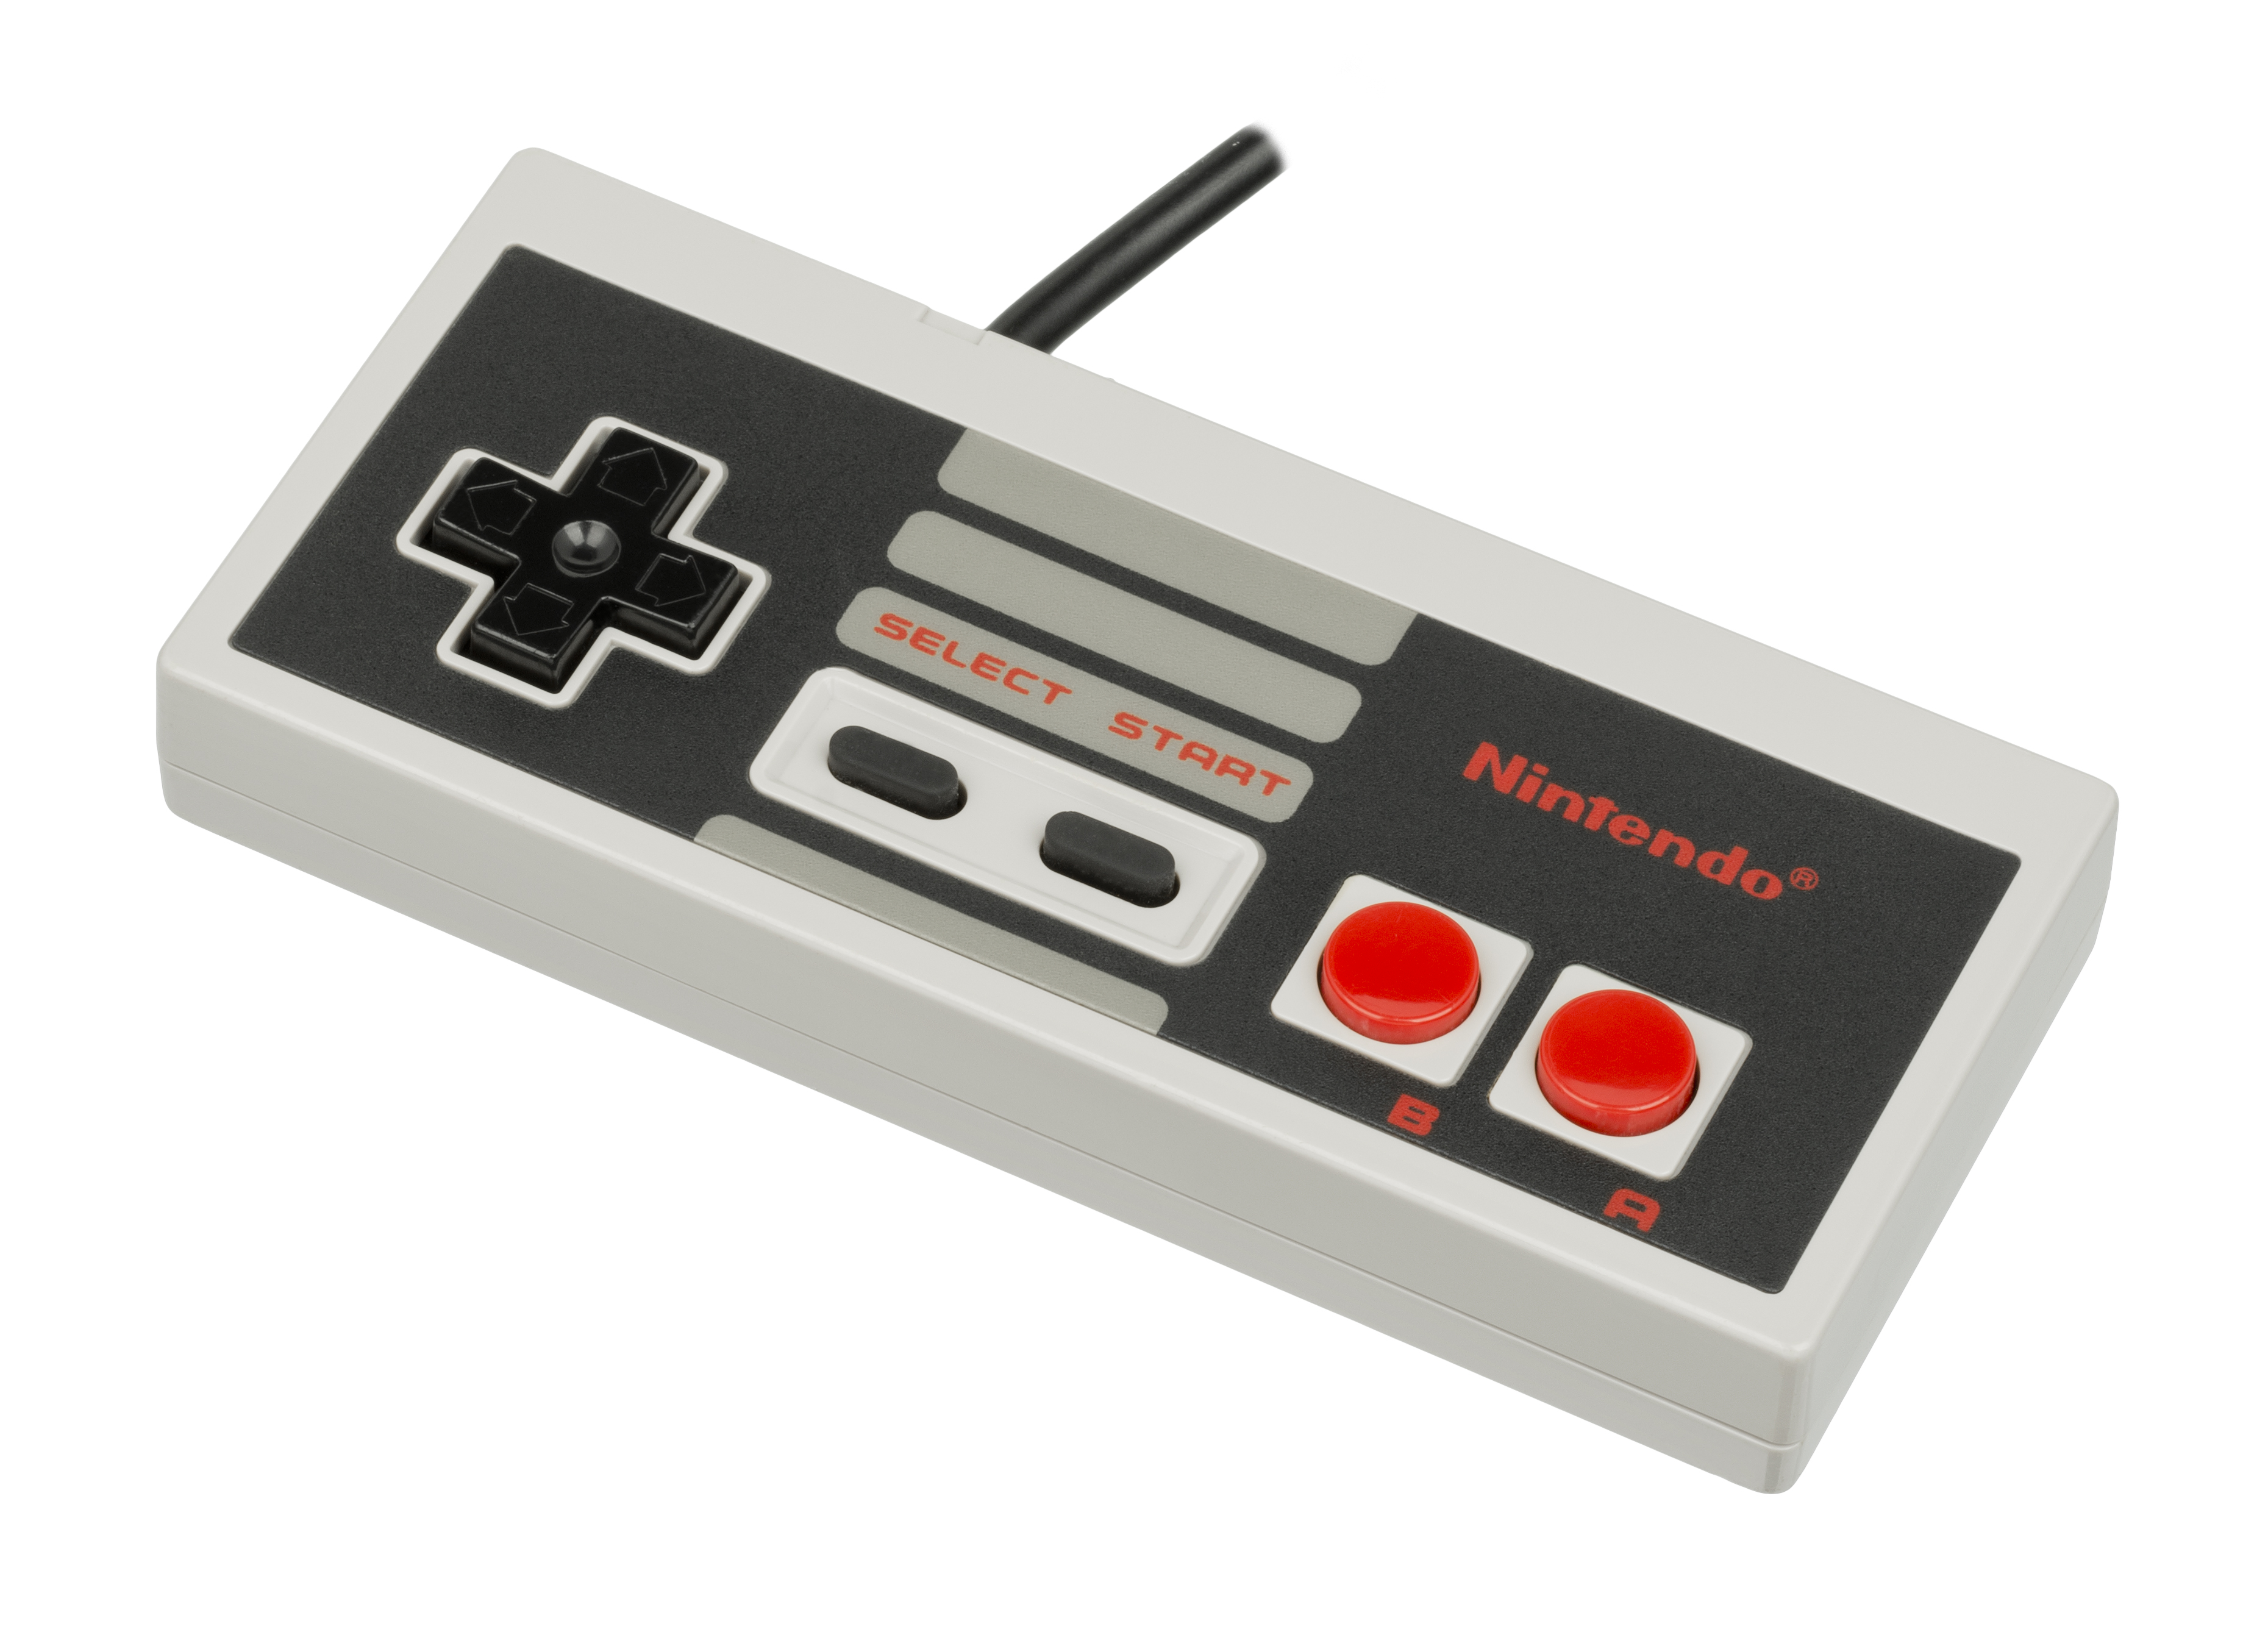
\includegraphics[width=0.5\textwidth]{images/nes-ovladac.jpg}
	\caption{Standardní ovladač konzole NES (foto \copyright~2016 Evan-Amos).}
	\label{fig:periferie-ovladac}
\end{figure}

Periferie jsou mapovány do paměti; čtení i~zápis tedy probíhají stejným způsobem, jako do každého jiného registru. První ovladač je mapován na adresu \$4016, druhý na sousední \$4017.

Při čtení jsou k~dispozici všechny tři piny, které jsou umístěny do jednotlivých bitů dle svého označení, tedy D0 na nejnižším bitu a tak dále. Tabulka~\ref{tab:periferie-cteci-piny} ukazuje, jakou mají piny funkci.

\begin{table}[ht!]
	\centering
	\caption{Funkce vstupních pinů portů konzole.}\label{tab:periferie-cteci-piny}
	\begin{tblr}{|Q[c,m]|Q[c,m]|}
		\hline
		Pin & Funkce \\
		\hline[2pt]
		D0 & Sériový výstup stavů tlačítek ovladače \\
		\hline
		D3 & Výstup světelného senzoru periferie Zapper \\
		\hline
		D4 & Stav spouště periferie Zapper \\ 
		\hline
	\end{tblr}
\end{table}

Stav tlačítek se vyčítá z~jediného bitu: D0. Jedná se o~sériový výstup osmibitového paralelně-sériového posuvného registru a~to, co je na jeho výstupu, záleží na stavu ovládacího klopného obvodu, který je k~dispozici pouze na nejnižším bitu adresy \$4016 (\$4017 je pouze pro čtení). Logickou jedničkou se aktivuje obnova stavu tlačítek do vnitřních registrů a~na výstupu je neustále stav jediného tlačítka (A). Přivedením nuly je pak možné postupně vyčíst hodnotu stisknutých tlačítek v~následujícím pořadí: A, B, Select, Start, Up, Down, Left, Right. Jelikož stisk tlačítka přivede na výstup logickou nulu, dochází k~dodatečné inverzi hodnoty tak, aby stisknuté tlačítko vracelo logickou jedničku a~puštěné logickou nulu~\cite{Nesdev:standard-controller}.

Po přečtení tlačítek vrací výstup logickou jedničku. To je způsobeno tím, že na sériový vstup posuvného registru (který se používá pro řetězení více takových posuvných registrů) je přivedeno nízké napětí (logická nula), což po dodatečné inverzi odpovídá logické jedničce. Pro další čtení je nutné opět obnovit stavy tlačítek~\cite{Nesdev:standard-controller}.

Standardní postup při čtení by se tedy dal shrnout takto:
\begin{enumerate}
	\item Zapsání logické jedničky do bitu 0 na adrese \$4016.
	\item Zapsání logické nuly do stejného místa.
	\item Postupné vyčítání osmi bitů ze sériového portu na adrese dle požadovaného ovladače (\$4016 či \$4017).
\end{enumerate}

\section{Audio Processing Unit}
\label{sec:APU}
Součástí procesoru Ricoh~2A03 je také zvukový syntezátor, přezdívaný jako Audio Processing Unit (APU).

APU obsahuje celkem čtyři konfigurovatelné syntezátory; dva generující pulzy, jeden generující trojúhelníky a~jednu jednotku generující šum. APU také umožňuje přehrávat krátké audiozáznamy ve formátu rozdílové PCM (pulzně-kódové modulaci). Pro analýzu a~implementaci byly zvoleny dva typy generátorů: pulzní a~šumový. APU se ovládá pomocí registrů přístupných procesoru. Přehled vybraných registrů relevantních k~bakalářské práci je uveden v~tabulce~\ref{tab:navrh-apu-registry}.

\begin{table}[ht!]
	\centering
	\caption{Registry APU.}\label{tab:navrh-apu-registry}
	\begin{tblr}{|Q[c,m]|Q[c,m]|}
		\hline
		Adresa & Funkce \\
		\hline[2pt]
		\$4000--\$4003 & Řízení generátoru pulzů 1 \\
		\hline
		\$4004--\$4007 & Řízení generátoru pulzů 2 \\
		\hline
		\$400C--\$400F & Řízení generátoru šumu \\
		\hline
		\$4015 & Stav APU \\
		\hline
		\$4017 & Čítač rámců \\
		\hline
	\end{tblr}
\end{table}


\subsection{Společné komponenty}
\subsubsection{Čítač rámců}
\label{sec:analyza-citac-ramcu}
Základem APU je takzvaný čítač rámců, které generuje hodinový signál pro všechny kanály. Navíc je tato jednotka schopná generovat přerušení s~frekvencí 60~Hz. Samotný čítač je řízen hodinami CPU dělenými dvěma, tudíž každý druhý cyklus procesoru je poslán hodinový cyklus i~do APU. Čítač lze nastavit registrem \$4017, který má následující strukturu: \texttt{MI------}. Je-li bit \texttt{M} roven 0, APU pracuje ve~čtyřkrokovém režimu, jinak pracuje v pětikrokovém režimu. Bit \texttt{I} je maskou přerušení; je-li tento bit nastaven, poté nebude přerušení vyvoláváno.~\cite{Nesdev:apu-frame-counter}

Čítač pracuje ve dvou režimech. Režim říká, v~kolika krocích bude APU pracovat a~co budou tyto kroky zahrnovat. Může pracovat buďto v~režimu sestávajícím ze čtyř, nebo z~pěti kroků. Krok je vykonán zhruba každých 3728~APU cyklů. Ve čtyřkrokovém řežimu je při každém kroku poslán hodinový signál do první skupiny komponent (generátor obálky a~čítač trojúhelníkového generátoru); každý druhý krok je poté poslán hodinový signál do druhé skupiny komponent (čítač délky a~regulátor period). V pětikrokovém režimu je hodinový signál do první skupiny zaslán ve všech krocích kromě čtvrtého, do druhé skupiny ve druhém kroku a~v~kroku pátém.~\cite{Nesdev:apu-frame-counter}

Podrobnější informace o~fungování čítače lze nalézt v~\cite{Nesdev:apu-frame-counter}.

\subsubsection{Mix}
Míchání všech výstupů probíhá v~mixu. Každý kanál má vlastní digitálně-analogový převodník, výsledkem je pak nelineární míchací schéma odhadnutelné například následujícím výpočtem převzatým z~\cite{Nesdev:apu-mixer}.

\[\textrm{výstup} = \textrm{suma\_pulz} + \textrm{suma\_tnd}\]
	
kde jsou jednotlivé složky vyjádřitelné jako
	
\[\textrm{suma\_pulz} = \frac{95,88}{\frac{8128}{\textrm{pulz1} + \textrm{pulz2}} + 100}\]

\[\textrm{suma\_tnd} = \frac{159,79}{\frac{1}{\frac{\textrm{trojúhelnik}}{8227} + \frac{\textrm{šum}}{12241} + \frac{\textrm{pcm}}{22638}} + 100}\]

\subsection{Generátor pulzů}
APU obsahuje celkem dva generátory pulzů. Oba se povolují zápisem hodnoty 1 do příslušných bitů ve společném registru \$4015; pro první kanál se jedná o~nejnižší bit a~pro druhý kanál druhý nejnižší bit. Každý z~generátorů se skládá z~pěti komponent:
\begin{itemize}
	\item generátor obálky signálu (viz~\cite{Nesdev:apu-envelope}),
	\item regulátor periody (označován jako sweep unit),
	\item 11bitový časovač řízený hodinami CPU dělenými dvěma (tudíž o~poloviční frekvenci),
	\item sekvencer (generátor průběhu) pracující v~osmi krocích,
	\item čítač délky (viz~\cite{Nesdev:apu-length-counter}).
\end{itemize}

Regulátory periody existují ve dvou jednotkách, každý pulzní kanál má svou jednotku. Ovládají se registry \$4001 pro první kanál a~\$4005 pro druhý. Oba mají stejnou strukturu: \texttt{EPPPNSSS}, kde \texttt{E} je povolení regulátoru (1 znamená povoleno), \texttt{PPP} je perioda děličky regulátoru, \texttt{N} určuje, zdali se se perioda přičítá (hodnota 0), nebo odčítá (hodnota 1), \texttt{SSS} je počet bitů k~posuvu. Je-li regulátor periody aktivní, upravuje hodnotu hlavního časovače v~těchto krocích:
\begin{enumerate}
	\item Načtení hodnoty 11bitového časovače a~posuv této hodnoty vpravo dle nastavení (bity \texttt{SSS}).
	\item Je-li bit \texttt{N} roven 1, poté je hodnota negována (první kanál narozdíl od druhého pracuje s~jedničkovým doplňkem, tudíž je hodnota ještě o~1 menší).
	\item Vypočtená (a~volitelně negovaná) hodnota je poté přičtena k~hlavnímu časovači.
\end{enumerate}

Regulátor periody má za jistých podmínek schopnost celý kanál vyřadit, což je včetně dalších podrobností fungování dokumentováno na stránce~\cite{Nesdev:apu-sweep}.

Třetí komponenta, 11bitový čítač, slouží k~taktování sekvenceru. Jeho hodnota je upravována pomocí dvou registrů: \$4002 (\$4006 pro druhý kanál) slouží k~nastavení výchozích spodních osmi bitů časovače; spodní tři bity \$4003 (\$4007 pro druhý kanál) poté nastavují výchozí horní tři bity časovače. 11bitová výchozí hodnota je perioda časovače. Každý APU hodinový takt je hodnota čítače dekrementována, po dosažení nuly se do čítače načte nakonfigurovaná výchozí hodnota a~sekvencer je posunut o~1~krok vpřed.~\cite{Nesdev:apu-pulse}

Sekvencer slouží ke generování průběhu signálu. APU obsahuje vnitřní tabulku o~čtyřech řádcích, kdy každý řádek reprezentuje jeden průběh signálu lišící se ve střídě. Jednotlivé hodnoty jsou omezeny pouze na 1 (maximální amplituda) a 0 (nulová amplituda --- ztlumení). Index řádku (a~tedy hodnotu střídy) lze nakonfigurovat pomocí registru dvou nejvyšších bitů registru \$4000 pro první, respektive \$4004 pro druhý kanál, což přesně odpovídá čtyřem možným hodnotám~\cite{Nesdev:apu-pulse}. Obrázek~\ref{fig:apu-signaly} ukazuje vzhled jednotlivých průběhů dle nakonfigurovaného indexu i~s~odpovídající hodnotou střídy v~procentech.

\begin{figure}[ht!]
	\centering
	\begin{tikztimingtable}[%
		timing/dslope=0.1,
		timing/.style={x=5ex,y=3ex},
		x=5ex,
		timing/rowdist=4ex,
		timing/name/.style={font=\sffamily\scriptsize}
		]
		\signal{0 (12,5~\%)} & L H 6L \\
		\signal{1 (25~\%)} & L 2H 5L \\
		\signal{2 (50~\%)} & L 4H 3L \\
		\signal{3 (75~\%)} & H 2L 5H \\
		\extracode
		\begin{pgfonlayer}{background}
			\begin{scope}[semitransparent ,semithick]
				\vertlines[black,dotted]{0.0, 1.0,2.0,...,8.0}
			\end{scope}
		\end{pgfonlayer}
	\end{tikztimingtable}
	\caption{Vzhled průběhů signálu pulzního kanálu APU.}\label{fig:apu-signaly}
\end{figure}

\begin{note}[Průběh signálu se 75\% střídou]
	Signál odpovídající indexu~3 na obrázku~\ref{fig:apu-signaly} je oproti ostatním signálům posunut. To je způsobeno tím, že sekvencer je sice inicializován na nultý krok, ale kroky počítá dolů, v~tabulce se tedy pohybuje opačným směrem a~signál je i~takto zvláštně generován~\normalfont{\cite{Nesdev:apu-pulse}}.
\end{note}

Sekvencer přivádí hodnotu vytvořenou generátorem obálky do mixu pouze tehdy, jsou-li splněny všechny následující podmínky:
\begin{itemize}
	\item aktuální hodnota kroku sekvenceru je 1,
	\item regulátor periody neztlumuje signál,
	\item hodnota čítače délky je vyšší než 0,
	\item hodnota 11bitového hlavního časovače je méně než 8.
\end{itemize}

\subsection{Generátor šumu}
Generátor šumu je mnohem jednodušší jednotkou nežli generátor pulzních signálů. Ve své podstatě jde o~pseudonáhodný generátor tónů. Skládá se z~následujících komponent:
\begin{enumerate}
	\item generátor obálky signálu (viz~\cite{Nesdev:apu-envelope}),
	\item 11bitový hlavní časovač,
	\item posuvný registr s~lineární zpětnou vazbou,
	\item čítač délky (viz~\cite{Nesdev:apu-length-counter}).
\end{enumerate}

Jediné dvě konfigurovatelné hodnoty specifické pro generátor šumu jsou nastavení režimu a~výchozí hodnoty časovače, obojí pomocí registru \$400E s~následující strukturou: \texttt{M---PPPP}. \texttt{M} je režim rozhodující o~bitu jdoucím do zpětné vazby, \texttt{PPPP} volba výchozí hodnoty (periody) hlavního časovače~\cite{Nesdev:apu-noise}. Konkrétní hodnota je určena dle tabulky, ta je k~nahlédnutí například v~\cite{Nesdev:apu-noise}.

Hlavní časovač funguje podobně jako u~pulzního kanálu, po dosažení nulové hodnoty dojde k~taktování tentokrát zpětnovazebního registru. Struktura registru je na obrázku~\ref{fig:apu-sum-LFSR}. Je-li nastaven bit M na 1, poté jsou zpětnovazební bity 0 a~6, jinak bity 0 a~1~\cite{Nesdev:apu-noise}.

% Inspirováno příspěvkem uživatele Excelsior na stránce https://tex.stackexchange.com/questions/592862/latex-using-tikz-to-draw-a-lfsr.
\begin{figure}[ht!]
	\centering
    \begin{tikzpicture}[node distance = 4mm and 0mm,
		box/.style = {shape=rectangle, draw, minimum size=2em, outer sep=0pt, on chain=#1},
		sum/.style = {shape=circle, draw, inner sep=0pt, node contents={$+$}},
		every path/.append style = {-latex'}
		]
		\def\scopeyshift{19mm}
		\begin{scope}[start chain=ch1 going left]
			\foreach \i in {0,...,14}{
				\node [box=ch1] (ch1-\i) {$s_{\i}$};
			}
			
			\node (c1) [color=lfsr,sum,below=of ch1-1,label=below:\texttt{M = 0}];
			\node (c6) [color=lfsr,sum,below=of ch1-6, label=below:\texttt{M = 1}];
			
			\draw (c1) edge (c6);
			
			\draw (ch1-0) -- ($(ch1-0) + (2,0)$) node (knot){};
			\draw[fill=black] ($(knot) + (-1,0)$) circle[radius=1pt];
			\draw[<-, >=stealth] (c1) -| ($(knot) + (-1,0)$);
			\draw (c6) -| ([xshift=0-5mm] ch1-14.west) -- (ch1-14);
			\draw[color=lfsr] (ch1-1) -- (c1);
			\draw[color=lfsr] (ch1-6) -- (c6);
		\end{scope}
	\end{tikzpicture}
	\caption{Zpětnovazební registr generátoru šumu.}\label{fig:apu-sum-LFSR}
\end{figure}

Generátor šumu přivádí hodnotu vytvořenou generátorem obálky do mixu za těchto podmínek:
\begin{itemize}
	\item aktuální hodnota nejnižšího bitu posuvného registru je 0,
	\item hodnota čítače délky je vyšší než 0.
\end{itemize}

\section{Existující řešení}
Emulátory konzole NES vznikaly již pro platformy dnes nepoužívané, například MS-DOS. Emulátorů NES vzniklo mnoho: pro různé platformy, s~různými funkcemi a~různými cíli. Přehledný seznam existujících implementací lze nalézt v~\cite{Nesdev:emus}. Emulátory lze rozdělit do tří skupin.

\emph{Precizní výkonné emulátory}: cílí především na co nejvěrohodnější napodobení NES a~zároveň nízkou náročnost na hardware. Tento typ emulátorů vznikal od samého začátku snah především proto, aby bylo možné spouštět původní programové vybavení pro NES (hlavně zábavní software) na novějších platformách co nejpřesněji s~ohledem na původní fungování na NES. Tomu odpovídá i~struktura kódu emulátoru. Využívají se různé triky, aby byla emulace věrohodná, ale zároveň nepříliš náročná, což vede k~nepřehlednému kódu (nejasné pojmenování funkcí a~proměnných, mnoho binárních operací bez dalších popisů\dots). Tím, že kód nebyl psán s~ohledem na modularitu, je často i~většina komponent silně provázaných. Komponenty nekomunikují přes abstrakci sběrnic a~signálních vodičů, ale bývá využívána ještě o~stupeň vyšší abstrakce. Dnes již tyto emulátory obsahují kromě prostředí pro samotné hraní i~například debugger a~jsou používány nejen hráči, ale díky své věrohodnosti i~jako simulátory pro vývojáře domácího softwaru pro NES (takzvaný homebrew vývoj). Pro účely bakalářské práce však vzhledem ke stylu napsaného kódu mohou posloužit pouze jako praktické ověření fungování konkrétních her a~porovnání s~implementací v~práci. Velmi věrohodným emulátorem je například fceux dostupný na GitHubu~\cite{fceux}.

\emph{Experimentální emulátory}: projekty (většinou) jednotlivců, kteří se chtějí dozvědět více o~fungování NES, popřípadě vytvořit emulátor nestandardním způsobem. Takových emulátorů vzniklo a~stále vzniká velké množství. Často jde o~nedokončené projekty, kde bylo cílem vytvořit jen prototyp či koncept. Takové emulátory se běžně nepoužívají ani pro hraní her, ani pro vývoj. Narozdíl od první jmenované skupiny již bývá kód přehledný, jsou totiž psány bez vyšších nároků na výkon, naopak s~vyššími nároky na přehlednost, mohou být tedy zajímavou inspirací i~co se kódu týče. Příkladem je projekt olcNES dostupný na GitHubu~\cite{olcNES}.

\emph{Komerční emulátory}. Tyto vznikly pouze pro distribuci konkrétních her na nové platformy přímo společností Nintendo (například acNES pro Game Boy a~GameCube, Virtual Console pro Wii, Wii~U a~3DS). Jedná se o~proprietární aplikace a nebyl pro ně zveřejněn zdrojový kód. Nemá tedy smysl je dále studovat, jelikož jde pouze o~komerční zábavní využití.

Bakalářská práce cílí výhradně do druhé jmenované skupiny; experimentální. Nemá smysl se pokoušet vyvíjet nový co nejpřesnější emulátor, takový zájem je mnohem lepší aplikovat příspěvkem do již existujících projektů. Ve skupině experimentálních emulátorů stále chyběl takový, který by se pokusil NES implementovat tak, že struktura kódu odpovídá i~reálné implementaci (hlavně co se modularity komponent a~komunikace mezi nimi týče). Navíc samotná existence experimentálních emulátorů ukazuje, že implementace emulátoru může být zajímavou příležitostí k~prozkoumání prakticky používané počítačové architektury a~vzdělání se v~této oblasti. Příkladem je emulátor olcNES, kdy autor vytvořil i~sadu videí, kde vysvětluje zajímavé principy fungování konzole. Bylo by tedy v~zájmu širší skupiny co nejvíce takový experimentální vývoj podpořit a~zpřístupnit tak, aby se potenciální vývojáři již mohli soustředit výhradně na implementaci emulovaného systému a~jeho komponent. Na základě toho byla do bakalářské práce zakomponována další myšlenka, a to vytvořit univerzální emulační platformu, která zařídí vše, co je sice k~běhu emulátoru potřebné, ale přímo se k~vývoji emulovaných komponent nevztahuje, a~až na této platformě vytvořit emulátor konzole NES.

%---------------------------------------------------------------
\chapter{Návrh}
%---------------------------------------------------------------
\epigraph{
	\enquote{Simplicity is prerequisite for reliability.}
}{\textsc{Edsger W. Dijkstra}}

Při analýze byly získány potřebné informace o~tom, z~čeho se NES skládá a~jak tyto komponenty fungují. Po analyzování systému je třeba navrhnout, jak jej prakticky implementovat. Vzhledem k~tomu, že je cílem projektu být co nejsrozumitelnější, je nutné brát v~potaz nejen návrh implementace samotného systému, ale i~emulační platformy, na které emulovaný systém poběží.

Nejprve je třeba navrhnout technologie, které se pro implementaci využijí. Dále je nutné navrhnout univerzální rozšiřitelnou platformu. Nakonec se za pomocí určených technologií a~platformy navrhne, jak implementovat samotnou konzoli NES.

Kapitola slouží jako přehled návrhových rozhodnutí, která vyvstala během řešení praktické části, a~jejich odůvodnění.

\section{Výběr technologií}
Na začátku vývoje je třeba vybrat správné nástroje tak, aby byl vývoj co nejefektivnější a~nejpohodlnější. Kromě jmenovaných požadavků je nutné brát v potaz také externí požadavky, které stanovuje jednak zadání, jednak výsledky samotného bádání v~analytické části.

\subsection{Programovací jazyk}
Zadání požaduje, aby byl emulátor implementován s~využitím principů objektově orientovaného programování. Vhodnost k~využití ve výuce pak znamená, že je třeba využít rozšířený jazyk, nebo takový jazyk, jehož syntaxe je běžným jazykům podobná. Nepřímo také vyplývá, že by mělo být možné výsledný kód spouštět na co největším množství platforem tak, aby byl emulátor, jakožto vzdělávací pomůcka, snadno dostupný. Nakonec je nutné se při výběru zaměřit na to, že se jedná o~implementaci počítačového systému. Zvolený jazyk by tedy neměl poskytovat příliš velkou abstrakci nad počítačovým hardwarem --- to by mohlo způsobit odstínění od vysvětlovaných principů.

Zvoleným jazykem pro implementaci je C++ ve verzi C++20. Splňuje totiž veškeré požadavky dané zadáním i~ze zadání vyplývajících:
\begin{itemize}
	\item podpora paradigmatu OOP,
	\item náklonnost k systémovému programování,
	\item umožňuje výběr míry abstrakce programátorem,
	\item podpora mnoha platforem,
	\item syntaxe podobná jiným rozšířeným C-like jazykům.
\end{itemize}

\subsection{Kolekce vývojových nástrojů}
\begin{definition}[Toolchain]
	Toolchain je anglický termín pro kolekci nástrojů využívaných při vývoji. Typicky se jedná o~soubor prostředí pro vývoj: textový editor pro psaní zdrojového kódu, kompilátor pro překlad do strojového kódu, linter pro kontrolu syntaktických chyb (dnes existují nástroje i~pro hledání různých sémantických chyb, například nástroj clang-tidy), debugger.
\end{definition}

Použití editoru se týká jen programátora, není tedy důležité toto rozhodnutí stanovit před začátkem projektu; nebude mít žádný vliv na výsledný projekt. Je však vhodné vyžadovat editor nabízející zvýrazňování syntaxe a~snadnou integrací s~dalšími částmi toolchainu, ať už se jedná o~pouhý editor, nebo celé integrované vývojové rozhraní (IDE). Pro účely projektu byl mezi dalšími možnostmi jako Visual Studio Code a~Qt Creator zvolen CLion (integrace s~CMake, přehledný grafický debugger, vestavěný linter).

Při návrhu toolchainu je brána v~potaz jednoduchost použití tak, aby šlo pokud možno vše zařídit automaticky: od stažení závislostí, přes kompilaci, testování i~generování dokumentace. Zároveň je z~hlediska přístupnosti vhodné, aby šel program zkompilovat na více než jedné platformě za pomocí stejného nástroje. Pro popis postupu kompilace se v~C/C++ projektech často používá Makefile; ten však není možné jednoduše použít na jiných platformách (například Windows). Pro abstrakci nad nástroji jako Make existuje CMake. Ten se jeví jako mnohem vhodnější řešení, jelikož umí vše vyžadované včetně generování Makefile, projektu pro Visual Studio, kompilování pro WebAssembly a~další. Bude tedy zvolen CMake.

\subsection{Správa zdrojového kódu}
Pro udržitelný vývoj většího projektu je vždy dobré mít přehled nad změnami, potažmo jednotlivými verzemi projektu. Možností verzování je několik. Nejjednodušší je prosté ukládání do několika složek v~souborovém systému, což ale brzy způsobí chaos a~špatně se synchronizují kolizní změny v~případě využití synchronizované složky. Standardem je dnes používání systémů správy verzí. Existují dvě možnosti: centralizovaná a~distribuovaná. Pro tento projekt byla zvolena distribuovaná, poněvadž umožňuje pracovat off-line a~téměř vždy existují alespoň dvě celé kopie repozitáře (lokální a~serverová). Konkrétním nástrojem byl zvolen Git, jelikož je standardem a~nabízí veškeré očekávané funkcionality distribuovaného systému pro správu verzí: lokální práci s~repozitářem, práce s~verzemi a~vývojovými větvemi, snadná komunikace se serverem, navíc i~jednoduché podepisování změň pomocí asymetrických kryptografických nástrojů.

Aby byl projekt v~rámci edukativnosti co nejdostupnější, je nutné použít veřejně přístupné úložiště i~s~možnostmi spolupráce a~přijímání změň od dobrovolníků. Velice známou platformou je \emph{GitHub}, který zdarma nabízí nejen umístění repozitáře, ale i~různé nástroje pro týmovou spolupráci, například trasování chyb a~úkolů. Vhod přijde i~možnost přímo na GitHubu jednoduše provozovat on-line dokumentaci.

\subsection{Dokumentace}
Dokumentace je nedílnou součástí projektu. Jednou z~možností, jak takovou dokumentaci tvořit, je průběžně vyplňovat externí textový dokument s~popisem kódu. Tato možnost je vhodná jen pro velice primitivní programy. Je možné totiž využít možností psaní dokumentace přímo v~kódu. Využívá se funkcionality komentářů, které jsou obohaceny o~možnosti vyplňování dalších údajů o~jednotlivých funkcích i~třídách; takovým komentářům se říká dokumentační. Z~takových komentářů lze pak jednoduše dokumentaci vygenerovat; proto je zvolena tato možnost.

Pro konkrétní zvolený programovací jazyk, C++, existuje nástroj \emph{Doxygen}. Ten za pomocí speciální syntaxe v~komentářích vygeneruje například i~popisy parametrů funkcí, návratových hodnot, popřípadě možných vyvolaných výjimek. Takto vygenerovanou dokumentace již je možné číst lokálně i~na serveru. Výstup programu Doxygen lze však dále zpracovat a~vytvořit přehlednější dokumentaci, což je velice důležité, pakliže je požadováno využití ve výuce. Pomocí nástrojů \emph{Breathe} a~\emph{Exhale} dojde k~převedení do formátu podporovaného nástrojem \emph{Sphinx}, který umožňuje přidávat další dokumentační stránky ve formátu \emph{reStructuredText} a~použití přehledných šablon (například šablona \enquote{ReadTheDocs} používaná pro mnoho open-source projektů, jmenovitě Admesh, Zoneminder a~další). Celý proces generování dokumentace lze automatizovat nástrojem CMake, což ještě zjednoduší průběžné úpravy dokumentace. Z~toho důvodu bude implementována také automatizace.

\subsection{Testování}
Aby byl zajištěn soulad s~požadavky, je nutné program testovat. Úkolem této části je stanovit požadavky na testy a~na tom základu navrhnout vhodné metodiky a~nástroje.

Ačkoliv je možné testování provést až na konci, je vhodné \emph{testovat průběžně}, aby bylo možné chyby diagnostikovat \emph{izolovaně}. Mohlo by totiž dojít k~situaci, kdy se chyba v~jedné komponentě projeví v~jiné, což přináší velmi těžce diagnostikovatelné problémy. Není však reálné provádět průběžné testy ručně, cílem tedy je navrhnout \emph{automatické testy}.

Spouštění testů v~základní formě vyžaduje akci programátora, což přináší riziko lidského faktoru v~podobě zapomenutí, především u~jednoduchých změn. Existují však nástroje, které umí i~spouštění testů provádět automaticky. Je rozumné se zaměřit především na \emph{testování před přijetím změn} --- nedovolit sloučit změny do hlavní vývojové větve v~repozitáři před tím, než se otestuje, zdali změny nevnesly nové chyby.

Specifikem bakalářské práce je fakt, že implementuje emulaci systému, od které se očekává, že bude věrně napodobovat emulovaný systém. Dalším požadavkem je proto možnost \emph{spouštět testy ve formě strojového kódu} pro danou platformu s~možností automatického vyhodnocení. Pro archaické systémy vzniklo již mnoho testů, které mají za úkol porovnat funkci s~reálným systémem. Sofistikované testy umožňují vybrat druh výstupu, kdy součástí bývá i~zápis výsledků do vybraného místa v~paměti.

Testy se dají provádět ručně i~automaticky. Jelikož je požadováno průběžné testování, je nejvhodnější co nejvíce testů automatizovat. To vyžaduje nástroj pro spouštění a~řízení testů. Součástí nástroje CMake je CTest, který je využit i~v~této práci. Pro samotné psaní testů již není třeba další komponenty, avšak využití dalších nástrojů může testování dále zjednodušit a~standardizovat jejich strukturu. Pro účely této práce byl zvolen Google Test. Umožňuje testovat konkrétní hodnoty, ověřovat vyvolané výjimky i~vytvářet znovupoužitelné struktury pro testování jednotným způsobem; díky tomu budou testy přehlednější. Výhodou je integrace Google Test se systémem CMake, proto je možné po úvodním nastavení testy vytvářet jako jednotlivé zdrojové soubory bez dalších úprav.

\section{Emulační platforma}
\label{sec:navrh-platforma}
\subsection{Stanovení požadavků}
\label{sec:navrh-pozadavky}

Aby byl projekt co nejuniverzálnější, bude v~rámci projektu vyvinuta platforma zjednodušující vývoj libovolného emulátoru historického systému. Na základě důkladné analýzy konzole NES je možné vytvořit seznam požadavků pro takovou platformu, což poslouží jako reference pro návrh.

Klíčovým požadavkem pevně souvisejícím s~principem fungování číslicového hardwaru je modularita, což představuje dělení na \emph{nezávislé komponenty}. Hardware vždy tvoří více nezávislých komponent. V~případě NES se i~ve vyšší úrovni abstrakce jedná třeba o~procesor, grafický čip a~kazetu. Samotné dělení na komponenty bude představovat implementace v~třídách v~rámci OOP, avšak je rozumné vyžadovat, aby měly komponenty stejné komunikační rozhraní tak, aby se daly univerzálně propojovat.

První požadavek přirozeně vytváří další: po navržení jednotného rozhraní pro komponenty musí být navržen \emph{způsob vzájemné komunikace} a~to ideálně takový, který odpovídá skutečné implementaci a~zároveň je rozumně efektivní.

Třetím požadavkem je vytvoření \emph{abstrakce celého systému}, v~jehož rámci se budou komponenty propojovat. Očekává se, že emulátor bude nabízet více různých systémů, proto je namístě vyžadovat jednotné rozhraní pro všechny systémy. Takové rozhraní by mělo obsahovat možnost řízení běhu systému přirozeně pomocí hodinového signálu; zároveň i~možnost, jak získávat různé informace o~systému.

Jakmile bude v~emulátoru existovat množina komponent jako součást systému, je možné uvažovat o~\emph{monitorování vnitřního stavu}. Bude nutné vytvořit jednoduchý způsob, jakým je možné pracovat s~celým systémem i~jednotlivými komponentami až na úroveň registrů a~obsahu paměti.

Kromě vnitřního stavu je přirozené očekávat, že bude emulátor nabízet i~běžně externě přístupné rozhraní, tedy reprezentaci \emph{vnějšího stavu systému}. Pro zachování univerzálnosti je nutné vytvořit univerzální řešení umožňující reprezentovat obrazový výstup (v~případě NES se jedná o~výstup herní grafiky z~čipu PPU na televizor; v~případě jiných soudobých systémů může jít o~výstup terminálu), zvukový výstup (u~NES je to zajištěno čipem APU; jinde, například u~Commodore~64 čipem 6581~SID, u~Atari čipem POKEY~\dots) a~uživatelský vstup (herní ovladače u~NES, klávesnice u~domácích mikropočítačů).

Pro shrnutí následuje seznam zjištěných požadavků:
\begin{itemize}
	\item dělení na nezávislé komponenty,
	\item způsob komunikace mezi komponentami,
	\item abstrakce celého systému zastřešujícího komponenty,
	\item monitorování vnitřního stavu komponent,
	\item reprezentace vnějšího stavu systému.
\end{itemize}

\subsection{Porovnání s~původními návrhy}
Požadavky přímo nevyplývající ze zadání se objevovaly postupně při vývoji několika prvních verzí emulační platformy; až posléze vznikl ucelený seznam popsaný v~části~\ref{sec:navrh-pozadavky}. Pro úplnost a~pochopení požadavků je vhodné připomenout nedostatky původních verzí.

\subsubsection{Platforma 1.0}
První platforma vznikla čistě pro účely experimentování. Hlavní cíl bylo rychle vytvořit funkční prostředí, ve kterém je možné implementovat emulovaný hardware. Velkou výhodou první platformy tedy bylo to, že byla implementována velice rychle.

Rozhraní komponent bylo různé a~systém byl ve své podstatě reprezentován třídou pro sběrnici. Tato vlastnost se projevila okamžitě při nutnosti testovat procesor 6502 zvlášť v~omezeném systému; bylo nutné buď duplikovat kód, nebo se kód stával rychle nepřehledným. I~z~toho důvodů byla jako požadavek pro další platformy stanovena především univerzální modularita.

Další velice nepříjemnou vlastností plynoucí z~absence modularity byla neexistence univerzálního způsobu prezentace stavu systému; vše bylo řešeno vystavením všech registrů a~pamětí přímo, nebo pomocí getterů. Často tedy docházelo k~porušení zapouzdření. Příklad takového špatného přístupu je v ukázce kódu~\ref{list:navrh-platforma1.0}.

\begin{listing}
	\caption{Zobrazení stavů registru \enquote{V} PPU na~platformě~1.0.}
	\label{list:navrh-platforma1.0}
	\begin{minted}{cpp}
ImGui::Text("V nameY: %u", m_bus.getPPU().m_internalRegisters.v.bits.nameY);
ImGui::Text("V nameX: %u", m_bus.getPPU().m_internalRegisters.v.bits.nameX);
ImGui::Text("V fineY: %u", m_bus.getPPU().m_internalRegisters.v.bits.fineY);
ImGui::Text("V coY: %u",   m_bus.getPPU().m_internalRegisters.v.bits.coarseY);
ImGui::Text("V coX: %u",   m_bus.getPPU().m_internalRegisters.v.bits.coarseX);
	\end{minted}
\end{listing}

Poslední velkou nevýhodou této platformy byla vázanost na jeden video i~audio backend. To znemožňovalo jednoduchou výměnu těchto komponent a~snadnou přenositelnost na jiné platformy. I~tato nevýhoda byla eliminována v~poslední verzi platformy.

Další nevýhody plynuly spíše pro uživatele. Jednou z~nich byla například i~absence systému dokování oken, což vždy vyústilo v~nepřehledné uživatelské rozhraní. Velice špatně byl řešen i~zvukový výstup, samotná emulace probíhala ve stejném vlákně jako callback pro zvukový ovladač, což vedlo k~trháním a~dalším zvukovým artefaktům.

\subsubsection{Platforma 1.5}
\label{sec:navrh-platforma1.5}
Mezikrok mezi platformami byl spíše prostorem pro vyzkoušení různých technik abstrakce grafického rozhraní. Jako první vznikla knihovna Elements, umožňující definovat soubor datových struktur k~ zobrazení bez závislosti nejen na grafickém backendu, ale i~na celé grafické knihovně. Projekt je dostupný na~\url{https://github.com/andreondra/elements}.

Myšlenkou bylo vytvořit třetí vrstvu abstrakce, jak ukazuje diagram~\ref{fig:navrh-abstrakce-grafiky}. Důvod takového uvažování vznikl z~prosté myšlenky. První platforma řešila zobrazování vnitřního stavu komponent externě, tudíž do nich musela nějakým způsobem zasahovat (například přes gettery). To způsobilo vazbu mezi více třídami; zobrazování bylo vázáno na vnitřní implementaci a~nabízené rozhraní dané komponenty, které nebylo jednotné. Bylo navrženo, že by komponenta měla být zodpovědná sama za zobrazování vnitřních hodnot tak, aby na tyto informace nemuselo být vázáno okolí. Komponenta by pouze zveřejnila nutné rozhraní pro komunikaci. Aby však komponenta nebyla vázána na konkrétní grafickou knihovnu, byla vytvořena idea další abstrakce.

\begin{figure}[ht!]
	\centering
	\begin{tikzpicture}[node distance=2cm] 
		\tikzstyle{uroven} = [rectangle, rounded corners, minimum width=5cm, minimum height=1cm,text centered, draw=black]
		\tikzstyle{arrow} = [thick,->,>=stealth]
		
		\node (elements) [uroven, fill=headbackgroundgray] {Elements};
		\node (gui) [uroven, below of=elements] {GUI knihovna};
		\node (backend) [uroven, below of=gui] {Grafický backend};
		
		\draw [arrow] (elements) -- (gui);
		\draw [arrow] (gui) -- (backend);
	\end{tikzpicture}
	\caption{Úrovně abstrakce práce s~grafikou.}\label{fig:navrh-abstrakce-grafiky}
\end{figure}

Úkolem knihovny Elements bylo poskytnout takové prostředky, pomocí kterých by programátor v~dané komponentě definoval, jaké proměnné a~v~jaké formě se mají zobrazovat v~grafickém rozhraní (otázka \emph{Co?}). Vše ostatní by řešila knihovna (otázka \emph{Jak?}). Třída představující abstrahovanou proměnnou a~další datové struktury byla označena jako Element. Každá část dat, která měla být reprezentována jakýmkoliv způsobem, by byla Element, ať už obsah registru, obsah paměti nebo surový grafický výstup. Tyto Elementy by byly strukturovány do balíčků označované jako Package. Takto bylo možné z~libovolné komponenty pomocí společného rozhraní \emph{getElements} získat abstraktní definici uživatelského rozhraní nezávislého na aktuální vnitřní reprezentaci.

Elementy umožňovaly získávat data nejen přímo, ale i~pomocí funkcí, bylo tedy možné hodnoty před zobrazením ještě upravit. Příkladem tvorby balíčku je kód ve~výpisu~\ref{list:navrh-elements-package}. Takový kód je prakticky spustitelný, v~repozitáři projektu je součástí příkladu v~souboru \texttt{main.cpp}.

\begin{listing}
	\caption{Tvorba Package z~Elementů.}
	\label{list:navrh-elements-package}
	\begin{minted}{cpp}
Elements::Package pkg("Test package", Elements::Types::Dock::LEFT);
pkg.addElements({
	new Elements::Text("Example text received via getter:"),
	new Elements::Text(getCurrentInstruction()),
	new Elements::Number("Number 8", &number8),
	new Elements::Number("Number 16", &number16),
	new Elements::Number("Number 32", &number32),
	new Elements::Number("Number Int", &numberInt),
	new Elements::Number("Number 64", &number64),
	new Elements::Separator(),
	new Elements::Number("Number dbl", &numberDbl),
	new Elements::Separator(),
	new Elements::Bool("Check me!", &exampleBoolean),
	new Elements::Separator(),
	new Elements::Memory("Example Mem", memory, sizeof(memory), 0, false),
	new Elements::Separator(),
	new Elements::Text("This is a beginning of custom rendering!"),
	new Elements::Display("Display Example", pixeldata, true),
	new Elements::Text("This is the end of custom rendering!")
});
	\end{minted}
\end{listing}

Definice proměnných a~dalších struktur k~zobrazení měla probíhat ve veřejné metodě třídy komponenty. Vznikly dva návrhy, jak by se definice mohla řešit: \emph{rekurzivně} a~\emph{registrací}.

Rekurzivní metoda počítala s~tím, že by funkce getElements vždy vrátila balíček, který by se začlenil do balíčku nadřazené komponenty. Takto by i~vznikla stromová struktura reprezentující hierarchii komponent. Registrační metoda by pak jako argument obdržela kontext, do kterého by vložila potřebné informace o~datech k~zobrazení bez nutnosti zanoření.

Nakonec se ukázalo, že spousta dalších funkcionalit knihovny Elements by už přímo musela souviset s~emulací (například Elementy pro řízení časování); také vývoj abstrakce nad všemi potřebnými typy zobrazovaných dat by zabral příliš mnoho času. Od vývoje knihovny bylo ustoupeno ve prospěch zcela nové platformy.

\subsection{Návrh platformy 2.0}
Úkolem platformy druhé verze bylo již vytvořit univerzální multiplatformní prostředí pro vývoj emulátorů; takto vznikla verze 2.0 označována jako Universal System Emulator. Průběžným vývojem se objevilo mnoho problémů a~jejich řešení, což vyústilo v~celistvý seznam požadavků uvedený v~\ref{sec:navrh-pozadavky}.

Celou platformu bude představovat třída~\emph{Emulator}. Součástí bude rozhraní pro přepínání systémů, jejich řízení a~také bude zastřešovat veškerá potřebná uživatelská nastavení. Zvýšenou péči v~návrhové části vyžaduje především systém pro nastavování preferencí. Jako první bude implementována možnost nastavit klávesy pro jednotlivé vstupy emulovaných systémů. Takové rozšíření pro knihovnu Dear~ImGui neexistuje, je tedy nutné jej naprogramovat. Jelikož je požadavek nastavování kláves využitelný i~v~jiných projektech, bude toto rozšíření vyvinuto zvlášť a~do projektu přidáno jako závislost. Jelikož se vývoj této knihovny (rozšíření) přímo netýká hlavního textu, je popsán v~příloze~\ref{apx:binder}.

\subsubsection{Modularita: třída Component}
První požadavek hovoří o~modularitě a~univerzálním rozhraní. Bude tedy implementována abstraktní třída \emph{Component}, která zastřeší veškeré komponenty obsažené v~systému, ať už to je složitější prvek jako procesor, nebo jednodušší prvky: paměti, sběrnice. Komponenty by měly poskytovat následující funkcionality:
\begin{itemize}
	\item práce s~piny (porty) na čipu --- (pouze) pomocí nich komponenta komunikuje s~okolím,
	\item práce s~metadaty --- každá komponenta má svůj název,
	\item inicializace --- navrácení komponenty do stavu po spuštění (restart),
	\item vytvoření rozhraní pro monitoring vnitřních i~vnějších stavů --- bude čistě v~režii komponenty, aby se nemusely interní informace vystavovat ven,
	\item rozhraní pro zvukový výstup.
\end{itemize}

Jediný problém, který při návrhu nastal, byla prostá otázka: co když není nějaká z~výše uvedených funkcionalit ve skutečném hardwaru k~dispozici? Možností bylo specializovat komponenty dle typu zařízení (pasivní: paměť, aktivní: procesor~\dots). Toto řešení bylo rychle zavrženo, anžto by popíralo myšlenku zcela unifikovaného rozhraní. Výsledné řešení je prozaické: zkrátka dojde k~navrácení \enquote{prázdných} hodnot (odpovídá to realitě, absence funkcionality totiž odpovídá prázdnotě). Konkrétní definice prázdnoty je implementačně závislá: prázdný kontejner, vyvolání výjimky, vrácení hodnoty přiřazené prázdnotě. Například prázdný kontejner může být vrácen tam, kde se vždy vrací skupina hodnot (seznam grafických prvků), vyvolání výjimky může být vhodné tam, kde by běh aplikace již neměl smysl (programátor zvolí neexistující port), speciální hodnota reprezentující prázdnotu může být navrácena u~jednoduchých typů (například je-li zvuk reprezentován párem čísel, absence zvuku odpovídá nule).

Díky existenci jednotného rozhraní bude možné s~komponentami pracovat hromadně; například zobrazování rozhraní bude spočívat v~zavolání stejné funkce napříč všemi komponentami v~jednom kontejneru.

\subsubsection{Komunikace: třídy Port a~Connector}
\label{sec:port-connector}
Při návrhu komunikace mezi komponentami musí být brána v~potaz i~reálná implementace. Lze vyjít z~hardwarového schématu konzole, které je obsahem příloh jako obrázek~\ref{fig:nes001-hw}. Na obrázku je patrné, že komponenty obsahují jednak adresní (A), datové (D) a~řídicí  (R/W) signály tvořící sběrnici, jednak jednotlivé signály (NMI, IRQ, INT\dots). Při komunikaci na sběrnici je vždy nějaký prvek, který je řídicí a~přes sběrnici (nebo přímo) přistupuje ke komponentám. Popsané chování lze emulovat tak, že řízená komponenta vystaví rozhraní, kterým ji lze ovládat, a~řídicí komponenta toto rozhraní využije. Pro řízenou komponentu bude vytvořena třída \emph{Connector} a~pro řídicí komponentu třída \emph{Port}. Řízená komponenta tedy nabízí několik konektorů, které si může řídicí třída připojit do svého portu, jehož prostřednictvím bude s~řízenou komponentou komunikovat. Využitím rozhraní odděleného od konkrétních komponent je možné komponenty propojovat libovolně, což bude důležité v~budoucích fázích projektu, kdy bude možné komponenty skládat do systému v~grafickém rozhraní. Bude tedy nutné mít možnost dostupné rozhraní enumerovat, což je díky takto univerzálnímu návrhu možné. Grafická reprezentace komunikace komponent je na obrázku~\ref{fig:navrh-komunikace-komponent}.

\begin{figure}[ht!]
	\centering
	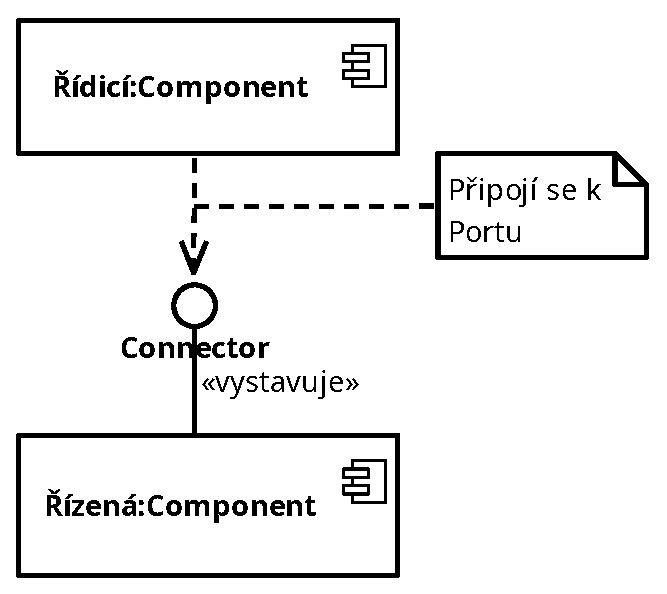
\includegraphics[width=0.4\textwidth]{images/port_connector.pdf}
	\caption{Komunikace komponent pomocí tříd Port a~Connector.}\label{fig:navrh-komunikace-komponent}
\end{figure}

Otázkou, kterou je třeba již v~návrhové fázi vyřešit, je zdali zůstane úroveň abstrakce u~jednotlivých signálu i~v~případě rozhraní pro sběrnici. Komunikaci je možné řešit stejně jako u~reálného hardwaru --- vystavení adresy a~příslušného řídicího stavu, poté přenos dat. Ukázalo se však, že ačkoliv by přístup věrně napodobil realitu, přinesl by zbytečné komplikace, přestože by výsledek byl stejný, jako u~abstraktnějších řešení. Případný zájemce o~vývoj vlastní komponenty by mohl být odrazen komplikovaností realistického přístupu. Výsledné řešení je kompromisem: ponechat možnost řízení na úrovni jednotlivých signálu, což by mohly navíc využít jednoduché signály (přerušení, hodinový signál); zároveň však i~zavést možnost, jak přenést všechny tři komunikační informace najednou (adresu, data i~řízení).

Sdružení komunikace přináší i~otázku, jak reprezentovat šířku komunikačního kanálu. Adresní sběrnice může být u~různých systémů různě široká, stejně tak i~datová. V~prvotních fázích bylo uvažováno, že šířka může být reprezentována pomocí šablon (templates), které C++ nabízí; adresa i~data by tak byla omezena zcela nativně datovým typem (například \texttt{uint8\_t}). Ukázalo se však, že mnohem lepší alternativou je použít dostatečně široký datový typ pro historické systémy (32 bitů) a~samotné ořezávání nastavit konstruktorem. Důvody jsou dva: obsahuje-li třída šablony, je nutné vše specifikovat v~hlavičkovém souboru (nepřehledné), navíc existují i~šířky sběrnic, pro které neexistují nativní datové typy (například adresní sběrnice pro komunikaci PPU s~kazetou je široká 14~bitů).

\subsubsection{Abstrakce systému: třída System}
Po vymyšlení reprezentace komponent a~jejich vzájemné komunikace je možné navrhnout abstrakci systému. Systém by měl poskytnout pro komponenty místo (stejně, jako jsou například v~NES v~krabičce na desce plošných spojů). To bude vyřešeno jednoduchým kontejnerem. Mělo by být možné pomocí systému řídit celou emulaci až na úrovni jednotlivých cyklů. Bude tedy dedikována metoda pro zaslání hodinového taktu do všech komponent.

Dále by měla existovat metoda umožňující běh v~reálném čase, která bude taktovací metodu využívat. Není možné běžící vlákno uspávat na časový úsek odpovídající prodlevě mezi jednotlivými takty o~frekvenci v~jednotkách megahertz, proto je vhodné takových taktů provést více. To, kolik taktů je nutné provést, záleží na četnosti volání zodpovědné metody. Nabízí se jednoduchý výpočet: $\textrm{počet\_volání} = \frac{f_{\textrm{taktovací}}}{f_{\textrm{volání}}}$.

Díky tomu, že komponenty budou součástí jednoho kontejneru, je vhodné vytvořit i~metody, které automaticky zařídí přenos všech grafických i~zvukových informací.

\subsubsection{Reprezentace vnitřních i~vnějších stavů}
Poslední dva požadavky spolu úzce souvisí. Pro reprezentaci grafických dat bude vybrána vhodná grafická knihovna. Možnosti jsou dle návrhových vzorů dvě: \emph{immediate mode} a~\emph{retained mode}. Dle prvního návrhového vzoru vykreslování probíhá přímo v~místě volání příslušných funkcí grafické knihovny. Dle druhého je tato zodpovědnost přenechána grafické knihovně. Požadavkem je jednoduchost a~možnost přímo reprezentovat požadované údaje, což naplňuje první návrhový vzor.

Nejpoužívanější a~nejlépe podporovanou immediate mode knihovnou je Dear ImGui.  Nabízí jednotné rozhraní nezávislé na subsystému řešící spolupráci s~konkrétní platformou (renderovací backend). Je možné vybrat mnoho backendů (OpenGL, SDL2, DirectX a~další). Platforma~1.0 používala jako backend knihovnu SDL2. Znalost konkrétního backendu přinesla široké možnosti optimalizace (práce přímo s~texturami), avšak i~určitá omezení v~podobě nemožnosti kompilovat pro platformy nepodporované tímto backendem.

Rozumnějším řešením je umožnit tyto backendy vybírat dynamicky a~pokud možno bez nutného zásahu programátora. Existuje projekt Hello~ImGui, který nabízí celý sestavovací skript postavený na CMake a~zároveň i~funkce zajišťující potřebné inicializace ovladačů, což přinese další zjednodušení i~flexibilitu. Pro bakalářskou práci bude zvoleno rozšíření označené jako ImGui~Bundle, které navíc obsahuje například funkcionality pro výběr souborů.

Díky použití knihovny Dear ImGui je možné přenechat vykreslování na každé komponentě, kdy každá funkce reprezentuje jedno okno. Aby mohly komponenty zobrazovat oken více, bude zodpovědná funkce vracet kontejner obsahující renderovací rutiny. C++ pro ukládání function-like objektů nabízí \texttt{std::function}. Objekty této třídy lze navíc ukládat do kontejnerů, což přesně odpovídá požadované funkcionalitě. Vrátí-li každá komponenta kolekci vykreslovacích funkcí, může systém tyto kolekce sloučit, zpracovat a~předat k~vykreslení.

Po návrh konkrétních vykreslovacích funkcí je nutné se zamyslet nad přístupem k~zobrazovaným datům. Vlastností immediate mode návrhového vzoru je to, že při vykreslování se přímo přistupuje k~datům. Není tedy možné bez dalších úprav zároveň vykreslovat a~emulovat. Existují tři možnosti:
\begin{enumerate}
	\item Nechat běžet vykreslování i~emulaci v~jednom vlákně.
	\item Provádět aktivity paralelně a~přístup k~datům chránit synchronizačním mechanismem (například mutex).
	\item Provádět aktivity paralelně a~data mezi vlákny synchronizovat.
\end{enumerate}

Paralelní přístup může lákat vyšším výkonem; mohl by však přinést zbytečně vyšší složitost platformy, přestože by neměl opodstatnění. Druhá možnost se ukázala jako zcela zbytečná, jelikož by téměř vždycky mohlo běžet jen jedno vlákno, tudíž by tento přístup odpovídal výkonu první varianty. To plyne z~faktu, že jeden hodinový cyklus může ovlivnit vnitřní stav všech komponent, tudíž vykreslovací vlákno by stejně muselo čekat. Třetí varianta by počítala s~tím, že by emulované komponenty vždy vkládaly vzorek svých vnitřních stavů do fronty, ze které by si je vybíralo vykreslovací vlákno. To odpovídá synchronizačnímu problému producent-konzument. Další problém by však nastal při požadavku na úpravu vnitřních stavů: již by muselo dojít k~zasílání i~druhým směrem a~musela by se tudíž vyvinout abstraktní knihovna podobná Elements popsané v~sekci~\ref{sec:navrh-platforma1.5}, což se ukázalo jako neekonomické. Nakonec byl zvolen první přístup, který dovoluje ve vykreslovacích funkcích specifikovat zobrazení požadovaných dat přímo a tudíž velice jednoduše. Například stav příznaku procesoru: \mintinline{cpp}|ImGui::Checkbox("C", &m_registers.status.c)|.

\subsubsection{Zvukový výstup}
Posledním problémem k~vyřešení je zvukový výstup. Zvukové zařízení (čip, karta) vyžaduje neustálý tok nových zvukových dat, který je vždy vyzvednut takzvaným callbackem běžícím ve zvláštním vlákně. Dojde-li k~přerušení, vznikají různé nepříjemné vedlejší efekty (chrčení, zrnění), které jsou uživatelem zaznamenatelné citelněji, nežli občasné zpomalení uživatelského rozhraní. Jedná se tedy o~reprezentaci zpracování v~reálném čase, kde deadline je při vyprázdnění vyrovnávací paměti obsahující vzorky k~přehrání.

Prvním úkolem bylo nalezení vhodné knihovny. Mezi požadavky patřila podpora více platforem (GNU/Linux, Windows, macOS, Emscripten), vestavěné filtry (dolní propust) a~vestavěné možnosti synchronizace (vyrovnávací paměť). Mezi kandidáty byly knihovny libsoundio, ffaudio, Maximilian, libnyquist a~miniaudio. Adeptem naplňujícím všechny zmíněné požadavky je pouze miniaudio.

Platforma by měla umožnit pracovat se zvukovým výstupem co nejjednodušeji. Veškerý zvukový výstup bude řešit zvláštní třída, která by měla miniaudio inicializovat, zaslat další vzorky k~přehrání a~zvuk spouštět i~zastavovat. Od komponent bude vyžadováno jen velice primitivní rozhraní odpovídající reálnému stavu: \emph{analogová} hodnota reprezentující amplitudu na výstupním portu. Veškeré časování bude zařízeno platformou, která se bude starat i~o~vyrovnávací paměť tak, aby nedošlo k~trhání zvuku. Očekávaný tok vzorků audia je znázorněn na diagramu~\ref{fig:navrh-audio-tok}. Takový mechanismus nabízí přímo knihovna miniaudio ve formě kruhového bufferu, který umí pracovat s~jedním producentem (emulační vlákno) a~jedním konzumentem (audio vlákno). Zde se opět ukazuje praktický výskyt synchronizačního problému producent-konzument, avšak je nutné oproti práci s~daty k~vykreslení aplikovat synchronizační mechanismy.

\begin{figure}[ht!]
	\centering
	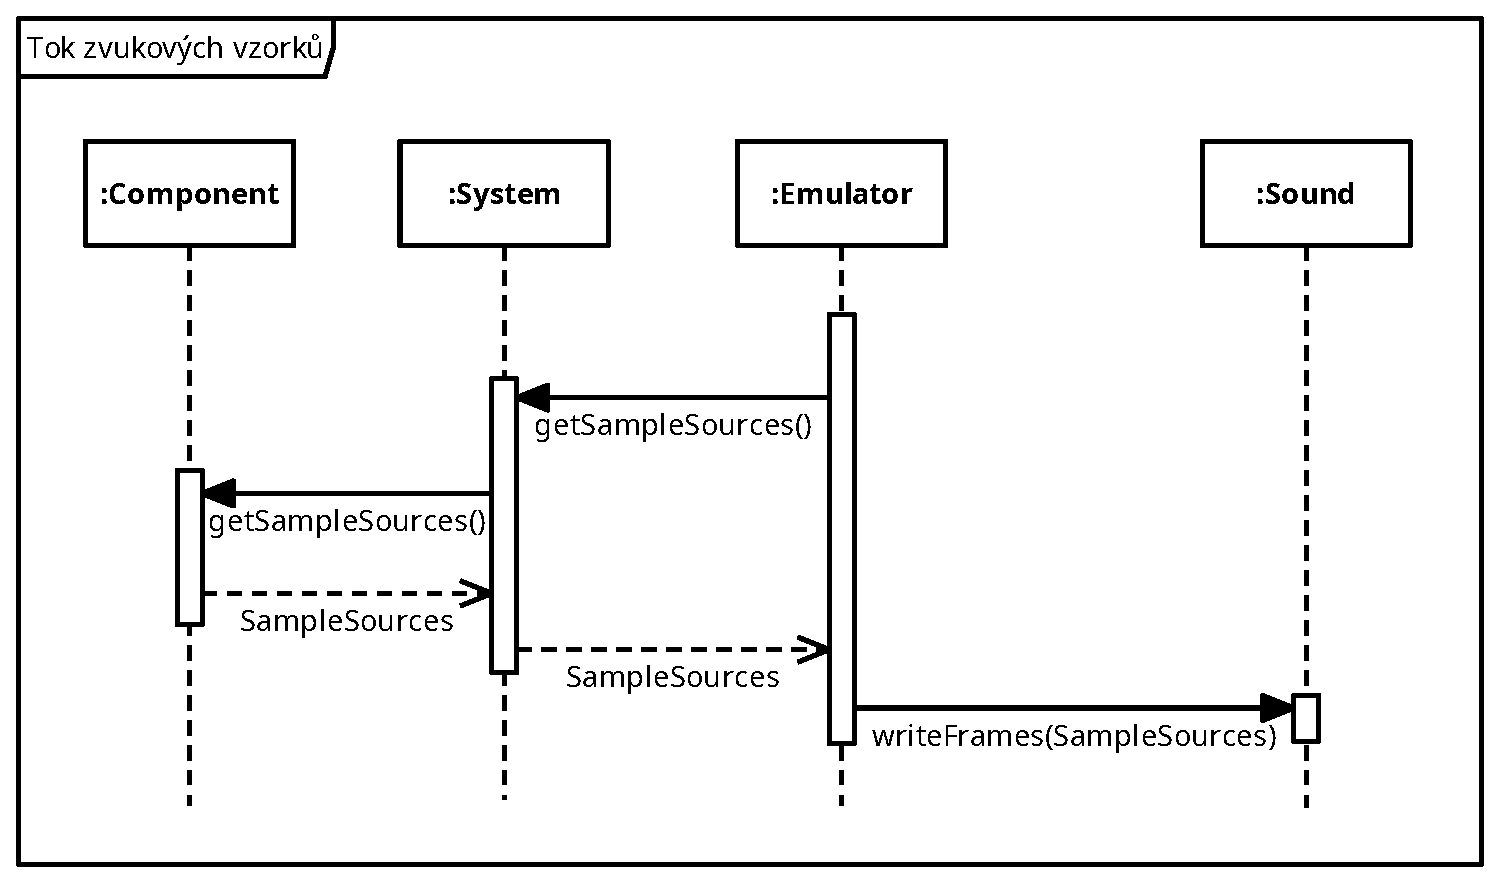
\includegraphics[width=1.0\textwidth]{images/tok_vzorku.pdf}
	\caption{Tok zvukových vzorků v~platformě~2.0.}\label{fig:navrh-audio-tok}
\end{figure}

\subsubsection{Shrnutí návrhu}
Celkově se tedy platforma bude skládat ze:
\begin{itemize}
	\item třídy Emulator, zastřešující celý projekt včetně možnosti nastavení kláves (knihovna ImInputBinder),
	\item třídy System, reprezentující systém, ve kterém se komponenty propojí pomocí tříd Port a~Connector,
	\item tříd Port a~Connector, reprezentující rozhraní řídicí, respektive řízené komponenty,
	\item třídy Component, reprezentující jednu komponentu, obsahující metody pro propojování portů a~konektorů a~pro export grafických i~zvukových vzorků,
	\item třídy Sound abstrahující veškeré nepříjemné aspekty práce se zvukem (inicializace, správa vyrovnávací paměti, přehrávání).
\end{itemize}

\section{Emulace konzole}
Emulační platforma samotná je jen nástrojem pro vývoj emulátorů --- nyní je třeba navrhnout jak implementovat konkrétní komponenty. Všechny komponenty budou potomky třídy Component pro dodržení myšlenky univerzálního rozhraní napříč celým emulátorem. Většina práce bude přenesení analýz, ale některým částem je třeba věnovat zvláštní pozornost, což je popsáno v~následujícím textu.

\subsection{Základní komponenty}
Základní komponenty je záhodno navrhnout univerzálně. Součástí NES je hlavní paměť a dvě sběrnice.

\subsubsection{Paměť}
Paměť je možné reprezentovat velice jednoduše: jedná se typicky o~blok bajtů za sebou, což lze reprezentovat polem. Paměť může reagovat na různé adresní rozsahy a~může být různě velká. Součástí konstruktoru tedy budou informace o~velikosti a~o~rozsahu. Díky existenci univerzálního rozhraní Port a~Connector stačí pouze do příslušných čtecích a~zapisovacích funkcí správně nastavit přístupy dle adresního rozsahu a~nastavené velikosti.

\subsubsection{Sběrnice}
Sběrnice bude pouhým prostředníkem mezi komponentami. Stejně jako u~skutečného hardwaru bude zápis na nějakou adresu vystaven na celou sběrnici --- to, jestli komponenty zareagují, je již na jejich vnitřní implementaci (například paměť reaguje jen na určitý rozsah, ale to sběrnici nemusí zajímat). Podobně jako u~zápisu i~adresa čtení bude vystavena na celou sběrnici. Může dojít ke konfliktům (reakci více komponent). Řešení konfliktů je ale otázka arbitračních mechanismů, ne sběrnice; bude tedy stačit, když se vezme v~potaz reakce první komponenty a~sběrnice s~arbitrací nebude reprezentována touto komponentou (u~NES arbitrace není třeba).

\subsection{Procesor 6502}
U~návrhu procesoru je nejdůležitější vymyslet, jakým způsobem se budou dekódovat instrukce. Ostatní bude již přenesením analýz do implementace.

Dekódování bude otázka dvou kroků: správně připravit data dle adresního režimu a~provést nad těmito daty příslušné operace. Instrukce včetně adresního režimu je jednoznačně reprezentována operačním kódem. Je tedy možné každému operačnímu kódu přiřadit jeden adresní režim a~jednu operaci. Adresní režimy jsou pro všechny instrukce společné, je tedy možné je implementovat zvlášť, nezávisle na operacích. Tím se ušetří mnoho práce, jelikož většina instrukcí existuje v~několika adresních režimech.

Operační znak je u~6502 jednobajtový. Je možné jej dekódovat několika způsoby:
\begin{enumerate}
	\item sada podmínek (\texttt{if-else}): to by přineslo dlouhý a~nepřehledný kód,
	\item přepínač (\texttt{switch}): je to lepší varianta než předchozí, stále ale bude nutné vytvořit mnoho řádků,
	\item vyhledávací tabulka: takto je řešeno i~dekódování v~procesoru, operační znak by mohl být pouhým indexem to takové tabulky, navíc lze tabulku implementovat přehledně tak, aby byla stejná, jako diagramy v~dokumentacích,
	\item postupné dekódování: to je možné u~takových instrukčních sad, kde mají operační kódy nějaké schéma (například procesor CHIP-8). ISA procesoru 6502 má sice nějaké schéma instrukcí, existují však výjimky, které by se stejně musely implementovat ručně, což by dekódování zpomalilo a~kód znepřehlednilo.
\end{enumerate}

Pro účely implementace procesoru 6502 v~tomto projektu bude zvolena možnost 3., jelikož je rychlá, přehledná i~věrně napodobující fungování původního hardwaru.

NES používá mírně upravenou verzi 6502 --- 2A03. Ta zároveň obsahuje zvukový syntezátor. Pro zajištění modularity bude zvukový syntezátor implementován ve zvláštní třídě a~2A03 bude pouze potomkem 6502 s~upravenými vlastnostmi.

\subsection{Grafický čip 2C02 (PPU)}
Grafický čip může být implementován na více úrovních abstrakce, což bude mít nejvyšší dopad na vykreslování pozadí.

Tím, že nametable ve videopaměti přímo reprezentuje část pozadí, může být tato část renderování vyřešena prostým vykreslením obsahu nametable. To však je možné pouze pro jednoduché hry nevyužívající posuv (scrolling). Aby bylo možné hrát více her, bude nutné vykreslování řešit po cyklech přesně tak, jak je popsáno v~analytické části. Pro projekt byla zvolena druhá možnost: sice je náročnější jak na implementaci, tak na výkon procesoru, avšak je věrohodnější a~bližší k~hardwarovému vzoru.

Další otázkou je reprezentace vnitřních pamětí grafického čipu. OAM~i~paletová paměť mohou být součástí PPU, jelikož je přímo používá pouze PPU (procesor musí přistupovat přes registry). Avšak videopaměť může být jak součástí PPU, tak kazety; záleží na tom, jaká konkrétní deska (mapper) byla použita. První myšlenkou je ponechat videopaměť v~PPU a~vystavit další rozhraní mezi PPU~a~kazetou, pomocí které bude kazeta PPU informovat, zdali se má vestavěná videopaměť používat a~jaký typ zrcadlení se má zvolit. Tím, že se ale kvůli zjednodušení sloučily adresní i~datové vodiče (viz část~\ref{sec:port-connector}), je vhodnější najít alternativní řešení. Tím je pevná integrace videopaměti do kazety --- stejně o~způsobu jejího používání vždy rozhoduje kazeta. Ačkoliv se takto přijde o~soulad s~hardwarovou reprezentací konzole, věrohodnost emulace to neovlivní, tudíž je možné tuto variantu zvolit.

\subsection{Kazeta a~mappery}
Kazeta jako taková je pouze obalem pro paměti a~řídicí desku, která rozhoduje o~mapování těchto pamětí (mapper). Takto to může být reprezentováno i~v~softwaru. Třída~\emph{Gamepak} (pojmenovaná po obchodním označení kazet pro NES) bude sloužit k~načtení souborů obsahujících potřebná data (ve formátu iNES) a~vybrání správného mapperu dle zjištěných metadat v~hlavičce souboru.

Reprezentace pamětí bude velice jednoduchá. Jelikož paměti nejsou přístupné jinde než v~rámci kazety, není třeba vytvářet podsběrnici a~reprezentovat je jako samostatné komponenty. 

Mapper již bude třeba reprezentovat sofistikovaněji. Pro práci s~mapperem je třeba jednotné rozhraní. Konkrétní implementace pak bude záviset na jednotlivých typech. Protože je v~C++ možné rozhraní implementovat pouze pomocí dědičnosti, budou jednotlivé mappery potomkem třídy Mapper. To, jaký konkrétní mapper je schován za rozhraním, bude známo jen při inicializaci, což ale stačí, jelikož vstupní parametry je třeba předat pouze při konstrukci mapperu. Dále tedy může být mapper zapouzdřen a~veškerá interakce bude probíhat přes jednotné rozhraní (čtení, zápis), což odpovídá realitě.

\subsection{Zvukový syntezátor APU}
Zvukový syntezátor je vlastně skupinou registrů, které říkají, jak se má generovat zvuk. Je tedy nutné se zamyslet, na jaké úrovni abstrakce bude emulace probíhat.

Je možné pouze využít parametry a~zvuk generovat jiným způsobem. Existují dva návrhy, které budou vysvětleny na jednom kanálu --- pulse. Tento kanál generuje čtvercový signál. Posílal-li by se čistý čtverec na výstup, mohlo by dojít k~nepříjemným artefaktům, které jsou způsobeny příliš rychlými změnami signálu (čtverec jsou skoky mezi žádným signálem a~signálem o~maximální amplitudě). Proto se nabízí tento signál aproximovat Fourierovou řadou pomocí sčítání sinusových signálů, vznikne tak mnohem hladší signál. Druhou možností je využít filtrovacích mechanismů, které nabízí zvolená knihovna miniaudio. Využije-li se filtr typu dolní propusti, výsledek bude stejný, ale méně výpočetně náročný. Navíc se takto věrně napodobí chování původního hardwaru: byl generován surový signál, který byl přes sadu filtrů dopraven až do reproduktorů televizoru.

\subsection{Herní ovladače}
Vzhledem k~jednoduchosti herních ovladačů není nutné vytvářet speciální návrh. Jde pouze o~sadu registrů. Jediné, co je nutné zajistit, je integrace s~knihovnou ImInputBinder, která zajistí přenos úhozů kláves do komponenty. Tím, že knihovna pracuje s~jednoduchým callbackem, jedná se pouze o~vrácení callbacku přes systém až do emulátoru.

\subsection{Integrace do platformy}
Pro přehled je na konec uveden diagram zachycující konkrétní realizaci emulátoru NES na platformě~2.0.

\begin{figure}[htp!]
	\centering
	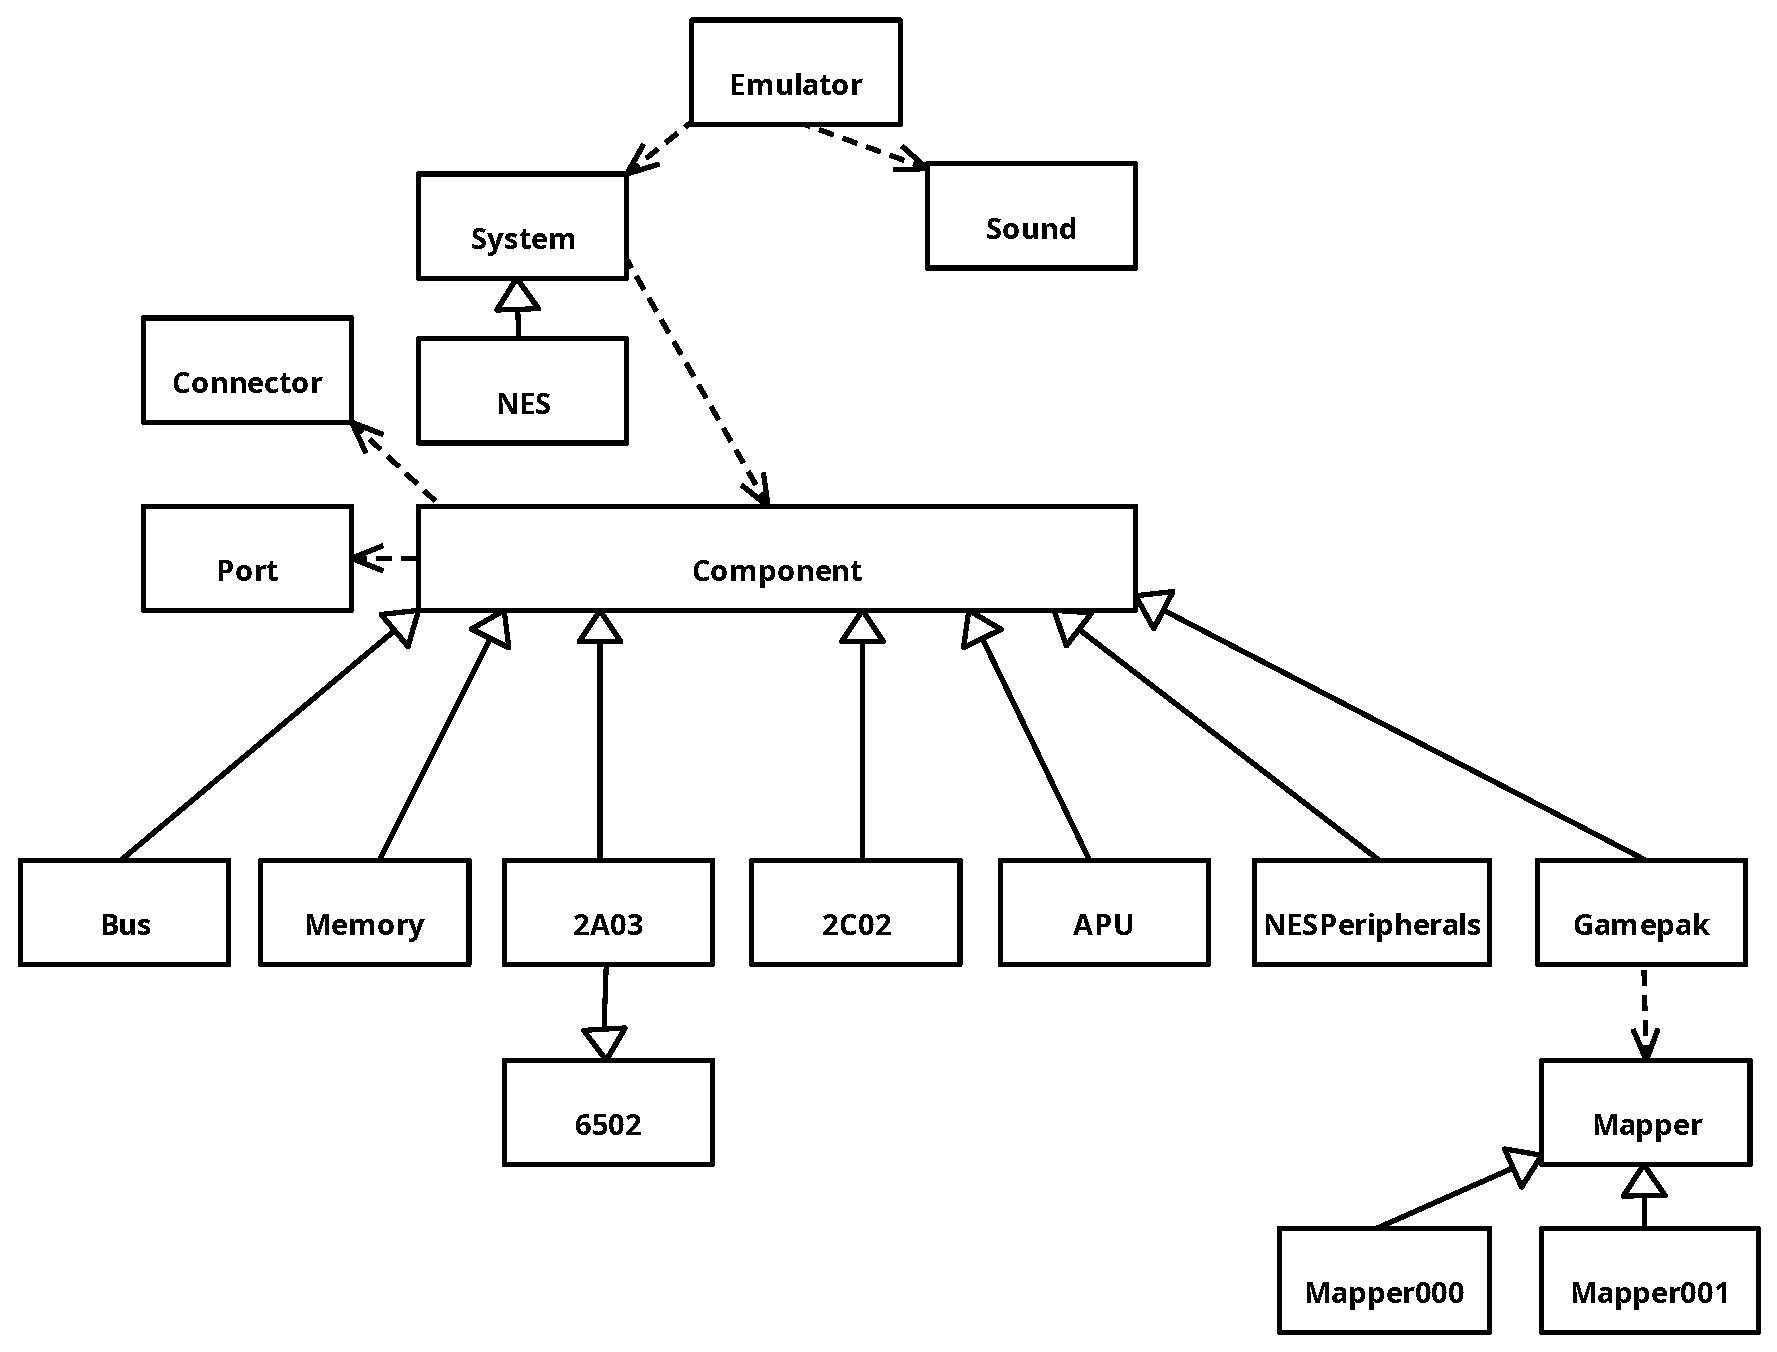
\includegraphics[width=1.0\textwidth]{images/navrh_prehled.pdf}
	\caption{Integrace NES do platformy 2.0.}\label{fig:navrh-prehled}
\end{figure}


%---------------------------------------------------------------
\chapter{Implementace}
%---------------------------------------------------------------
\epigraph{
	\enquote{If you love what you do and are willing to do what it takes, it's within your reach.}
}{\textsc{Steve Wozniak}}

Po analýze a~navržení následuje praktická část, kdy se projekt implementuje pomocí vybraných technologií. 
Úkolem kapitoly implementace je provést strukturou projektu a~poukázat na zajímavé řešené problémy.

Praktická část probíhala v~několika fázích po dobu 2~let. Během prvních fází byly postupně vytvořeny emulované komponenty, v~dalších byla vytvářena emulační platforma v~několika verzích (které jsou porovnány v~návrhové kapitole v~sekci~\ref{sec:navrh-platforma}). Poslední verze emulační platformy, nazvaná jako Universal System Emulator, byla vytvářena posledního půlroku studia na fakultě.

Projekt je podrobně dokumentován. V~případě většího zájmu o~implementační detaily je důrazně doporučeno paralelně studovat zdrojový kód; je obohacen o~mnoho dokumentačních komentářů, z~nichž lze snadno vygenerovat dokumentaci ve formátu kompatibilním s~webovými prohlížeči (HTML dokument).

\begin{note}[Zápis signatur metod]
	U některých metod a~funkcí jsou vynechány signatury (značeno trojtečkou), pakliže to není v~textu relevantní a~je důležitý pouze název. Patřičné signatury i~s~popisky lze nastudovat ve zdrojovém kódu.
\end{note}

\section{Struktura projektu}
Projekt je k~dispozici na veřejném repozitáři na platformě GitHub~\cite{Golasowski2023:use}. Součástí repozitáře je celá platforma, implementace NES i~dokumentace a~veškeré pomocné nástroje. Obrázek~\ref{fig:impl-struktura-projektu} strukturu projektu znázorňuje graficky.

\begin{figure}[p!]
%	\centering
	\dirtree{%
		.1 .github\DTcomment{skripty pro kontinuální sestavování na platformě GitHub Actions}.
		.1 cmake\_src\DTcomment{další pomocné skripty nástroje CMake}.
		.1 docs\DTcomment{zdrojový kód dokumentace}.
		.1 graphics\DTcomment{různá pomocná grafika (loga a další)}.
		.1 include\DTcomment{C++ hlavičkové soubory odpovídající zdrojovým souborům}.
		.1 src\DTcomment{zdrojový kód projektu}.
		.2 components\DTcomment{zdrojové kódy jednotlivých komponent}.
		.3 Gamepak.
		.4 Gamepak.cpp\DTcomment{emulace kazety NES}.
		.4 Mapper.cpp\DTcomment{abstrakce mapperů}.
		.4 Mapper000.cpp\DTcomment{emulace mapperu 0}.
		.4 Mapper001.cpp\DTcomment{emulace mapperu 1}.
		.3 2A03.cpp\DTcomment{emulace čipu 2A03}.
		.3 2C02.cpp\DTcomment{emulace grafického čipu 2C02 (PPU)}.
		.3 6502.cpp\DTcomment{emulace procesoru 6502}.
		.3 APU.cpp\DTcomment{emulace audio čipu APU}.
		.3 Bus.cpp\DTcomment{univerzální emulace sběrnice}.
		.3 Memory.cpp\DTcomment{univerzální emulace přepisovatelné paměti}.
		.3 NESPeripherals.cpp\DTcomment{emulace periferií NES}.
		.3 Trigger.cpp\DTcomment{konvertor mezi typy signálů}.
		.2 systems\DTcomment{zdrojové kódy systémů}.
		.2 Component.cpp\DTcomment{abstrakce komponenty}.
		.2 Connector.cpp\DTcomment{abstrakce konektoru}.
		.2 Emulator.cpp\DTcomment{hlavní třída zastřešující celou platformu}.
		.2 Port.cpp\DTcomment{abstrakce portu}.
		.2 Sound.cpp\DTcomment{rozhraní nad zvukovým ovladačem}.
		.2 System.cpp\DTcomment{abstrakce systému}.
		.2 Tools.cpp\DTcomment{pomocné funkce}.
		.1 tests\DTcomment{testy projektu}.
		.2 testfiles\DTcomment{pomocné testovací soubory}.
		.2 unit\DTcomment{testy jednotlivých komponent}.
		.1 .gitignore\DTcomment{seznam ignorovaných souborů systémem git}.
		.1 CMakeLists.txt\DTcomment{soubor projektu systému CMake}.
		.1 COPYING\DTcomment{licence GPL-3.0}.
		.1 README\DTcomment{základní informace k~projektu}.
		.1 main.cpp\DTcomment{hlavní kompilační jednotka projektu}.
	}
	\caption{Popis struktury projektu.}\label{fig:impl-struktura-projektu}
\end{figure}

\section{Emulační platforma}
Princip fungování emulační platformy bude rozebrán od té nejnižší úrovně --- komponenty --- až na celou emulační platformu.

\subsection{Komponenty}
Každá komponenta, která má být součástí platformy, musí splňovat rozhraní definované abstraktní třídou \mintinline{cpp}|Component|, což se v~C++ provede snadno principem dědění: \mintinline{cpp}|class mojeKomponenta : public Component|. Úkolem této abstraktní třídy je poskytnout komponentě vše potřebné pro začlenění do libovolného systému i~pro samotný běh emulace a~debugging. Pro komunikaci s~ostatními komponentami jsou připraveny následující metody:
\begin{itemize}
	\item \mintinline{cpp}|connect(...)|: připojení řízené komponenty,
	\item \mintinline{cpp}|disconnect(...)|: odpojení řízené komponenty,
	\item \mintinline{cpp}|getConnector(...)|: získání rozhraní pro jinou řídicí komponentu.
\end{itemize}

Dále pro zjednodušení komunikace s~uživatelem slouží tyto metody:
\begin{itemize}
	\item \mintinline{cpp}|getGUIs()|: získání seznamu popisů grafického rozhraní debuggerů,
	\item \mintinline{cpp}|getSoundSampleSources()|: získání seznamu funkcí pro načítání zvukových vzorků,
	\item \mintinline{cpp}|getInputs()|: získání seznamu podporovaných uživatelských vstupů (klávesnice, ovladače).
\end{itemize}

Jsou připraveny i~další metody pro sjednocení životního cyklu komponent. Takovými funkcemi jsou \mintinline{cpp}|init()| pro uvedení komponenty do stavu po přivedení napájecího napětí (hard reset, nebo také studený start) a~\mintinline{cpp}|initRequested()| jakožto možnost komponenty požádat o~inicializaci celého systému (například po výměně ROM je nutné obnovit programový čítač procesoru, což se například u~6502 standardně děje při resetu).

Vývojář komponenty má za úkol implementovat funkce \mintinline{cpp}|getGUIs(), init()| a~volitelně další. Většinou je také nutné definovat vnější rozhraní, což se provádí v~konstruktoru a~příklad je uveden v~dokumentaci k~projektu.

Nejdůležitějším přínosem platformy je jednoduchost tvorby grafického rozhraní a~zvukového výstupu. Nejprve je demonstrován proces tvorby rozhraní na zjednodušené komponentě ve výpisu kódu~\ref{list:use-konfigurace-gui}. Vše, co je potřebné definovat, je obsaženo v~jediné funkci, v~rámci níž je možné definovat libovolné množství lambda funkcí reprezentujících vykreslovaná okna. Tyto funkce jsou pak předány v~kontejneru typu vektor i~s~metadaty (kategorie, název okna, popřípadě preferovaný dok, do kterého se má okno umístit).

\begin{listing}
	\caption{Příklad konfigurace grafického rozhraní pro komponentu emulující procesor.}
	\label{list:use-konfigurace-gui}
	\begin{minted}[tabsize=2]{cpp}
std::vector<EmulatorWindow> MujProcesor::getGUIs() {
	
	std::function<void(void)> debugger = [this](){
		
		// Definice obsahu okna.
		// ==========================================================
		ImGui::SeparatorText("Current instruction");
		ImGui::Text("Mnemonic: %s",         m_instruction.mnemonic);
		ImGui::Text("Cycles: %u",           m_cycles);
		ImGui::Text("Size: %u B",           m_instruction.instrLen);
		ImGui::Text("Address mode: %s",     getAddressMode().c_str());
		ImGui::Text("Remaining cycles: %u", m_cycles);
		
		ImGui::SeparatorText("Registers");
		ImGui::InputScalar("PC", ImGuiDataType_U16, &m_registers.pc,
		nullptr, nullptr, "%x", ImGuiInputTextFlags_CharsHexadecimal);
		// ...zkraceno...
		ImGui::InputScalar("Y", ImGuiDataType_U8, &m_registers.y,
		nullptr, nullptr, "%x", ImGuiInputTextFlags_CharsHexadecimal);
		
		ImGui::SeparatorText("Status flags");
		ImGui::Checkbox("C", &m_registers.status.c);
		// ...zkraceno...
		ImGui::SameLine();
		ImGui::Checkbox("N", &m_registers.status.n);
		
		ImGui::SeparatorText("Interrupt vectors");
		ImGui::Text("NMI at: 0x%x",     VECTOR_NMI);
		ImGui::Text("RESET at: 0x%x",   VECTOR_RST);
		ImGui::Text("IRQ/BRK at: 0x%x", VECTOR_IRQ);
		ImGui::SeparatorText("Interrupt status");
	};
	
	// Definice seznamu oken.
	return {
		EmulatorWindow{
			.category =    m_deviceName,
			.title =       "Debugger",
			.id    =       getDeviceID(),
			.dock  =       DockSpace::LEFT,
			.guiFunction = debugger
		}
	};
}
	\end{minted}
\end{listing}

Mnohem jednodušší je předávání zvuku k~přehrání. Tím, že veškerou rutinní práci odvede již implementovaná specializovaná třída \mintinline{cpp}|Sound|, stačí v~rámci funkce \mintinline{cpp}|getSoundSampleSources()| předat dvouvzorkový rámec (jeden vzorek pro levý a~jeden pro pravý reproduktor) reprezentující amplitudu, která by byla v~reálné komponentě na analogovém výstupu. Pro většinu emulovaných zvukových čipů je to tedy otázka předání hodnot z~již hotové funkce generující zvuk (popřípadě i~převedení formátu, nejedná-li se o~výstup v~plovoucí desetinné čárce v~rozsahu $[-1, 1]$). Ukázka implementované funkce pro čip APU je obsažena ve výpisu kódu~\ref{list:use-konfigurace-audia}.

\begin{listing}
	\caption{Implementace rozhraní pro přístup ke zvukovým datům.}
	\label{list:use-konfigurace-audia}
	\begin{minted}[tabsize=2]{cpp}
SoundSampleSources APU::getSoundSampleSources() {
	
	return {
		[&](){
			
			float sample =  output();
			// Mono vystup, proto jsou oba vzorky stejne.
			SoundStereoFrame frame{sample, sample};
			return frame;
		}
	};
}
	\end{minted}
\end{listing}

\subsection{Práce se zvukem}
Pro co nejjednodušší zpřístupnění zvukového výstupu byla vytvořena třída \mintinline{cpp}|Sound|. Tato třída má velice jednoduché rozhraní: \mintinline{cpp}|start()| a~\mintinline{cpp}|stop()| pro spuštění či zastavení přehrávání dodaných zvukových rámců a~\mintinline{cpp}|writeFrames()| pro dodání rámců k~přehrání. Je zcela abstrahováno to, jaký zvukový ovladač se ve skutečnosti používá, jak dochází ke zpracování jednotlivých zvukových rámců i~jak probíhá komunikace s~audio callbackem (a tedy dodávání zpracovaných rámců) --- to vše zajistí platforma tak, aby byla vývojáři emulátoru zpříjemněna a~zjednodušena práce.

Třídu \mintinline{cpp}|Sound| spravuje platforma (třída \mintinline{cpp}|Emulator|). Při nahrání emulovaného systému dojde k~vytvoření grafu reprezentujícího tok zvukových vzorků při jejich zpracování. Počátek grafu je tvořen vstupními body, jejichž počet závisí na počtu zdrojů zvuku. Vstupní body se integrují zcela automaticky bez zásahu vývojáře systému, pakliže správně implementoval funkci pro získání seznamu zdrojů zvuku. Všechny vstupní body jsou smíchány a předány dalšímu uzlu, což je filtr typu dolní propust. Ten je použit proto, aby byly omezeny příliš velké změny amplitud, které vedou k~nepříjemnému praskání na výstupu (v~reproduktorech či sluchátkách). Nakonec je smíchaný~a~filtrovaný výsledný zvuk přiveden na výstup. Graficky je tento tok znázorněn na obrázku~\ref{fig:impl-zvuk-tok-dat}.

\begin{figure}[ht!]
	\centering
	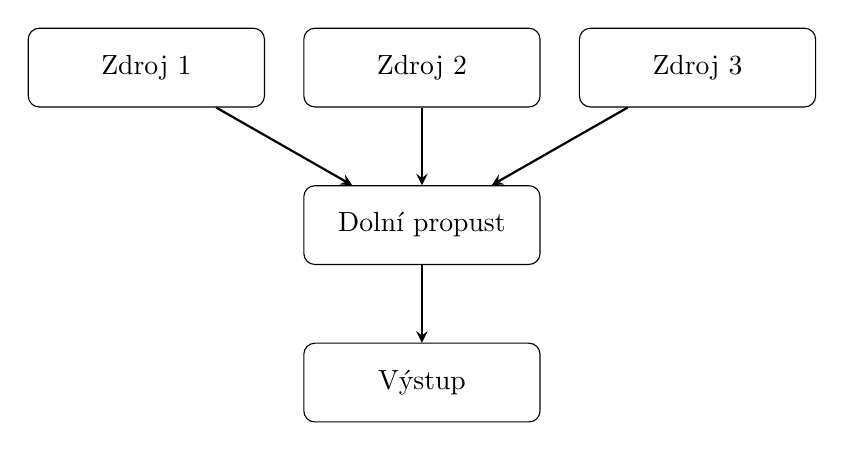
\begin{tikzpicture}[node distance=2cm] 
		\tikzstyle{uroven} = [rectangle, rounded corners, minimum width=3cm, minimum height=1cm,text centered, draw=black]
		\tikzstyle{arrow} = [thick,->,>=stealth]
		
		\node (zdroj1) [uroven] {Zdroj 1};
		\node (zdroj2)[uroven, right of =zdroj1, xshift=1.5cm]{Zdroj 2};
		\node (zdroj3)[uroven, right of=zdroj2, xshift=1.5cm]{Zdroj 3};
		\node (dp)[uroven, below of=zdroj2]{Dolní propust};
		\node (out)[uroven, below of=dp]{Výstup};
		
		\draw [arrow] (zdroj1) -- (dp);
		\draw [arrow] (zdroj2) -- (dp);
		\draw [arrow] (zdroj3) -- (dp);
		\draw [arrow] (dp) -- (out);
	\end{tikzpicture}
	\caption{Schéma toku zvukových dat ze 3~zdrojů.}\label{fig:impl-zvuk-tok-dat}
\end{figure}

Jak lze pozorovat na implementaci mechanismu zpracování zvuku, je jen na vývojáři emulovaných komponent, potažmo systému, kolik zdrojů zvuku platformě poskytne. Je možné vše smíchat vlastním způsobem a~klidně za celý systém předat jen jeden zdroj, nebo předat několik zdrojů za každou komponentu a~přenechat veškeré míchaní na platformě. Samozřejmě je možné nepředávat žádný zdroj, přehrávání zvuku tak nebude k~dispozici.

\subsection{Komunikace komponent}
Jak bylo popsáno v~návrhové části, komunikace komponent probíhá pomocí tříd~\mintinline{cpp}|Port| a~\mintinline{cpp}|Connector|. Nejprve je ukázáno, jak se jednotlivé třídy používají, poté je vysvětlen princip jejich implementace.

Chce-li komponenta zveřejnit port, pomocí nějž by řídila ostatní komponenty, vybere typ portu a přidá jej jako datovou položku třídy. Poté v~konstruktoru přidá port do seznamu zveřejněných portů: \mintinline{cpp}|m_ports["nazev_portu"] = &m_mujPort|. Dle vybraného typu portu jsou pak k~dispozici různá rozhraní. Typ \mintinline{cpp}|DataPort| je emulací kombinace datových, adresních a~řídicích vodičů, umožňuje komunikovat pomocí metod \mintinline{cpp}|uint32_t read(uint32_t address)| pro přečtení dat z~vybrané adresy a~\mintinline{cpp}|void write(uint32_t address, uint32_t data)| pro zápis dat na zvolenou adresu. Typ \mintinline{cpp}|SignalPort| je poté emulace surových signálů. Umožňuje nastavit logickou úroveň na pomyslném vodiči pomocí \mintinline{cpp}|void set(bool active)|, popřípadě pouze zaslat jeden pomyslný signální pulz (změnu logické hodnoty; je na připojené komponentě, jak jej interpretuje) pomocí \mintinline{cpp}|void send();|. Nastavení logické úrovně je použitelné pro komunikaci s~úrovňovými detektory (u~6502 port IRQ), poslání signálu je poté užitečné pro hranové detektory (u~6502 port NMI).  Do portu je možné připojit konektor, takové rozhraní mají oba typy portů společné: \mintinline{cpp}|void connect(std::weak_ptr<Connector> connector)|. Port po připojení konektoru zkontroluje, zdali je v~konektoru definováno požadované rozhraní a~pokud ano, je možné pomocí portu komunikovat s~připojenou komponentou přes její konektor.

Chce-li být komponenta řízena jinou komponentou, musí naopak zveřejnit konektor, toť jest typ třídy \mintinline{cpp}|Connector|.  Konektory jsou v~komponentách ukládány do kontejneru typu \mintinline{cpp}|std::map|. Deklarace i~definice probíhá v~konstruktoru. Výpis kódu~\ref{list:use-konfigurace-konektoru} ukazuje, jak lze nadefinovat jak typ konektoru poskytující datové rozhraní, tak typ konektoru poskytující signální rozhraní; prezentovaný kód by byl uveden v~konstruktoru.

\begin{listing}
	\caption{Definování konektorů různých typů.}
	\label{list:use-konfigurace-konektoru}
	\begin{minted}[tabsize=2]{cpp}
	// Konektor poskytujici signalni rozhrani emulujici hranovy detektor.
    m_connectors["CLK"] = std::make_shared<Connector>(SignalInterface{
		.send = [this](){
			CLK();
		}
	});
	
	// Konektor poskytujici signalni rozhrani emulujici urovnovy detektor.
	 m_connectors["IRQ"] = std::make_shared<Connector>(SignalInterface{
		.set = [this](bool active) {
			IRQ(active);
		}
	});
	
	// Kontektor slouzici pro pripojeni na hlavni sbernici.
	// V prikladu jsou k dispozici dva registry na dvou adresach,
	// z toho druhy je pouze pro cteni.
	m_connectors["BUS"] = std::make_shared<Connector>(DataInterface{

		.read = [&](uint32_t address, uint32_t & buffer) {
			if(address == 0x4016) {
				buffer = m_register1;
				return true;
			} else if(address == 0x4017) {
				buffer = m_register2;
				return true;
			} else {
				return false;
			}
		},
	
		.write = [&](uint32_t address, uint32_t data) {
			if(address == 0x4016){
				m_register1 = data;
			}
		
			// (Registr 2 pouze pro cteni, neni potreba zadny kod.)
		}
	});
	\end{minted}
\end{listing}

\begin{note}[Důvod použití chytrých ukazatelů]
	Jak bylo popsáno výše, port je vždy lokální datová položka komponenty, kdežto konektory se předávají napříč komponentami. Bylo tedy nutné vymyslet, jak se budou komponenty předávat. Myšlenka surového ukazatele byla v~rámci dodržování principů bezpečné práce s~pamětí zavržena. Předává-li se totiž surový ukazatel, nemusí být příliš zřejmé, kdo spravuje ukazovaný objekt. Dobrou volbou není ani \mintinline{cpp}|std::shared_ptr|, jelikož je sémanticky vlastníkem pouze komponenta, které konektor patří.
	
	 Nejideálnější volbou by byl \enquote{chytrý} pozorující (observing) ukazatel. Je to vlastně jen sémantický obal nad surovým ukazatelem, který však jasně říká, že se pracuje s~ukazatelem na objekt spravovaný někým jiným. Ten je však v~C++ zatím součástí plánovaných rozšíření, tudíž ve jmenném prostoru \mintinline{cpp}|std::experimental|, což není zcela vhodné používat ve stabilním kódu~\normalfont{\cite{Brown2014:observing-ptr}}. V~projektu byl proto použit pro předávání dalším komponentám \mintinline{cpp}|std::weak_ptr|, jakožto kompromisní (ale stabilní) řešení.
\end{note}

\subsection{Systémy}
Po vyvinutí komponent je možné začít tvořit komplexní systémy využívající tyto komponenty. K~tomuto účelu slouží třída \mintinline{cpp}|System| zajišťující jednotné rozhraní i~jednotný přístup k~definování emulovaných systémů.

Systém obsahuje metody pro postupování emulací po různě velkých úsecích, například po jednotlivých taktech hlavních hodin lze postupovat pomocí \mintinline{cpp}|doClocks()|. Je zajištěno~i~rozhraní pro běh v~reálném čase: \mintinline{cpp}|doRun(...)|. Tyto metody musí implementovat vývojář systému.

Systém obsahuje mnoho předpřipravených metod. Týká se to především práce se společným rozhraním komponent. Jsou to metody pro získání definic grafického rozhraní všech komponent (\mintinline{cpp}|getGUIs()|), získání všech zdrojů zvuku (\mintinline{cpp}|getSampleSources()|), definice všech dostupných uživatelských vstupů (\mintinline{cpp}|getInputs()|), popřípadě \mintinline{cpp}|init()| pro skupinovou inicializaci všech komponent. Aby měl systém povědomí o~komponentách v~systému, je nutné tyto komponenty přidat do připraveného kontejneru typu vektor s~identifikátorem \mintinline{cpp}|m_components|. Poté je již funkční výchozí implementace zmiňovaných metod.

\begin{note}[Grafický editor systému]
	V~současné verzi platformy se počítá s~vytvářením systému pouze vyvinutím dalších tříd, které se poté ručně zakomponují do platformy přidáním do nabídky v~hlavní třídě \mintinline{cpp}|Emulator|. Návrh komponent proběhl však velice pečlivě tak, aby bylo možné do budoucna implementovat třídu reprezentující univerzální systém, který bude implementovatelný grafickým rozhraním. Počítá se s~využitím editoru grafů, pomocí nějž půjde skládat systém jak na úrovni komplexních komponent (procesor, grafický čip), tak na úrovni hradel.
\end{note}

Pro implementaci funkčního systému musí vývojář také definovat propojení komponent, vhodné je definovat i~název systému. To se provádí v~konstruktoru systému. Díky univerzálnímu návrhu je to velice jednoduché. Příklad propojení ukazuje výpis kódu~\ref{list:use-propojeni}, v~němž je procesor řídicí prvek komunikace na sběrnici (master) a~RAM figuruje na sběrnici jako ukázka řízeného zařízení (slave).

\begin{listing}
	\caption{Propojení komponent v systému.}
	\label{list:use-propojeni}
	\begin{minted}[tabsize=2]{cpp}
		// Definice nazvu systemu.
		m_systemName = "Bare 6502";
		
		// Pripojeni RAM ke sbernici.
		m_bus.connect("slot 1", m_RAM.getConnector("data"));
		// Pripojeni sbernice k procesoru.
		m_cpu.connect("mainBus", m_bus.getConnector("master"));
		
		// Pridani komponent do metadat tak, 
		// aby byly funkcni predimplementovane metody.
		m_components.push_back(&m_bus);
		m_components.push_back(&m_RAM);
		m_components.push_back(&m_cpu);
	\end{minted}
\end{listing}

\subsection{Platforma}
Platforma je reprezentována třídou \mintinline{cpp}|Emulator|. Tato třída definuje společné grafické rozhraní (správa systémů, nastavení přiřazení kláves a~další). Zajišťuje také načítání systémů a~předávání zvukových dat třídě \mintinline{cpp}|Sound| a~grafických dat knihovně Dear~ImGui.

\section{Emulované komponenty}
Po dokončení emulační platformy je možné implementovat jednotlivé komponenty a~integrovat je s~platformou. V~rámci bakalářské práce byly vyvinuty jednak komponenty univerzální, jednak komponenty specifické pro konzoli NES.

\subsection{Univerzální komponenty}
Aby mohl procesor komunikovat s~více komponentami, je potřebná \emph{sběrnice}. Koncept sběrnice je použitelný ve více systémech, proto je záhodno sběrnici navrhnout univerzálně. Téměř veškerá \enquote{logika} sběrnice spočívá v~komunikaci, proto je také většina kódu v~definici konektoru. Ukázkou toho, jak se dá emulovat univerzální čtecí a~zápisová logika sběrnice pro řídicí zařízení na platformě 2.0 (USE) je znázorněna ve výpisu kódu~\ref{list:use-sbernice}.

\begin{listing}
	\caption{Definice čtecí a~zápisové logiky sběrnice využívané například procesorem.}
	\label{list:use-sbernice}
	\begin{minted}[tabsize=2]{cpp}
 m_connectors["master"] = std::make_shared<Connector>(
	
	DataInterface {
	
		.read = [&](uint32_t address, uint32_t & buffer) {
	
			// Pokus o cteni na vsech zarizenich.
			// Zaznamena se pouze odpoved prvniho zarizeni 
			// (primitivni arbitracni mechanismus).
			for(auto & device : m_devices) {
				if(device.readConfirmed(address & m_addrMask, buffer)) {
					buffer &= m_dataMask;
					return true;
				}
			}
			
			return false;
		},
	
		.write = [&](uint32_t address, uint32_t data) {
	
			// Provedeni zapisu na vsechna zarizeni.		
			for(auto & device : m_devices)
				device.write(address & m_addrMask, data & m_dataMask);
		}
	}
);
	\end{minted}
\end{listing}

Podobně jako sběrnice je i~\emph{paměť} komponentou, kterou je možné využít i~v~rámci jednoho systému hned několikrát, z~čehož vyplývá, že je vhodné ji také implementovat univerzálně. Stejně jako v~případě sběrnice se většina logiky nachází právě v~definici konektoru, neboli rozhraní pro zařízení, které bude k~paměti přistupovat. Zde již stojí za zmínku fakt, že k~paměti lze pomocí definovaného konektoru přistupovat buď přímo, tedy tak, že se přímo k~paměti připojí například procesor, nebo nepřímo přes sběrnici, pakliže má procesor ve svém adresním prostoru více zařízení, což je případ procesoru 6502 v~konzoli NES. Zkrátka univerzálnost návrhu umožňuje s~komponentami pracovat modulárně tak, jako by se jednalo o~komponenty skutečné. Aby nebyla demonstrována jen tvorba konektorů, kterou lze prostudovat ve zdrojovém kódu práce, je v~případě paměti ukázán způsob, jakým se definuje počáteční stav komponenty pomocí metody \mintinline{cpp}|init()| ve výpisu kódu~\ref{list:use-init-pamet}.

\begin{listing}
	\caption{Definice počátečního stavu emulované paměti.}
	\label{list:use-init-pamet}
	\begin{minted}[tabsize=2]{cpp}
void Memory::init() {
	std::fill(m_data.begin(), m_data.end(), m_defaultValue);
}
	\end{minted}
\end{listing}

Kromě paměti a~sběrnice byla implementována ještě další komponenta, \mintinline{cpp}|Trigger|, která slouží jako převodník mezi adresním a~signálním konektorem. Využití je například v~případě, kdy potřebujeme mapovat signální vstup do paměti. V~reálném systému se to například používalo pro testování reakcí na přerušení procesoru 6502, kdy se vstupy pro přerušení (IRQ a~NMI) mapovaly do adresního rozsahu procesoru tak, aby kód mohl zápisem do předem daných adres uměle-programově přerušení vyvolat (viz sekce~\ref{sec:test-procesor}). Implementace tohoto převodníku spočívá jen v~definici rozhraní konektoru v~konstruktoru, což lze v~případě zájmu podrobněji prostudovat ve zdrojovém kódu.

\subsection{Komponenty NES}
\subsubsection{Procesor 6502 a~varianta 2A03}
První implementovanou komponentou byl \emph{procesor 6502}. Před započetím implementace instrukcí bylo nutné implementovat způsob dekódování instrukcí. Jak bylo vybráno v~návrhové části, vhodnou možností je vyhledávací tabulka. Při implementaci záznamu vyhledávací tabulky bylo zváženo vše, co je třeba uchovávat spolu s~instrukcí. Jak bylo zjištěno v~analýze, instrukce existuje ve více variantách dle adresního režimu, má své zkrácené označení a~zároveň může její zpracování trvat různě dlouho, což je měřitelné ve strojových cyklech. Strukturu záznamu ukazuje výpis kódu~\ref{list:use-6502-zaznam}, kde byla pro jednoduchost přidána ještě délka instrukce. Celou tabulku lze nalézt ve zdrojovém kódu.

\begin{listing}
	\caption{Záznam instrukční tabulky procesoru 6502.}
	\label{list:use-6502-zaznam}
	\begin{minted}[tabsize=2]{cpp}
typedef struct {
	// Oznaceni OZ.
	char mnemonic[4];
	// Ukazatel na adresni rezim.
	uint8_t (MOS6502::*addrMode)();
	// Ukazatel na funkci nalezici instrukci.
	uint8_t (MOS6502::*instrCode)();
	// Delka instrukce v bajtech.
	uint8_t instrLen;
	// Pocet cyklu potrebnych k vykonani instrukce.
	uint8_t cycles;
} instruction_t;
	\end{minted}
\end{listing}

Instrukce i~adresní režimy procesoru 6502 byly implementovány jako třídní metody. Příklad absolutního adresního režimu a~implementace instrukce pro sčítání s~přenosem (add with carry, ADC) je ve výpisu kódu~\ref{list:use-6502-instrukce}. Dále bylo nutné implementovat stav po spuštění (opět přetížením metody~\mintinline{cpp}|init()|) a~dále obsluhu přerušení tak, aby věrně napodobila skutečné chování procesoru 6502, jelikož je klíčová ke správné synchronizaci komponent. Zpracování přerušení probíhá v~několika krocích; protože je dosti rozsáhlé, je zde zevrubně popsáno včetně názvů relevantních metod. Opět je doporučeno nahlédnout do zdrojového kódu v~případě zájmu o~hlubší pochopení.

\begin{listing}
	\caption{Ukázka implementace absolutního adresního režimu 6502 a~instrukce ADC.}
	\label{list:use-6502-instrukce}
	\begin{minted}[tabsize=2]{cpp}
// Absolutni adresni rezim.
uint8_t MOS6502::ABS(){
	m_addrAbs = m_mainBus.read(m_registers.pc) |
	            (m_mainBus.read(m_registers.pc + 1) << 8);
	m_registers.pc += 2;
	return 0;
}

// Instrukce add with carry (scitani obsahu pameti, akumulatoru a priznaku C).
uint8_t MOS6502::ADC(){
	
	uint8_t memoryValue = m_mainBus.read(m_addrAbs);
	
	bool memoryNegative = (memoryValue & 0x80) == 0x80;
	bool accNegative    = (m_registers.acc & 0x80) == 0x80;
	
	uint16_t result = (uint16_t)m_registers.acc +
	                  (uint16_t)memoryValue +
	                  (uint16_t)m_registers.status.c;

	m_registers.status.c = (result & 0x100) == 0x100;
	result &= 0xFF;
	m_registers.status.z = result == 0x0;
	m_registers.status.n = (result & 0x80) == 0x80;
	
	if(memoryNegative != accNegative)
		m_registers.status.v = 0;
	else
		m_registers.status.v = memoryNegative == accNegative && 
	                           memoryNegative != m_registers.status.n;
	
	m_registers.acc = result;
	
	return 1;
}
	\end{minted}
\end{listing}

Při obdržení požadavku na přerušení (obvykle pomocí relevantního konektoru) dojde k~nastavení vnitřního signálu pomocí metod dle typu přerušení (\mintinline{cpp}|NMI(), IRQ(bool active)|). Během vykonávání strojového cyklu ve funkci \mintinline{cpp}|CLK()| se vyhodnotí priorita přerušení a~podle toho je naplánováno další vykonávání: buď se vykoná standardně další instrukce, nebo se provede přerušení. Je-li naplánováno přerušení, zavolá se metoda \mintinline{cpp}|irqHandler()|, nebo \mintinline{cpp}|nmiHandler()|, ve kterých se provede stejný sled kroků jako u~skutečného procesoru (záloha kontextu na zásobník, přepsání programového čítače hodnotou vektoru přerušení) a~další vykonávanou instrukcí je pak první instrukce rutiny obsluhy přerušení.

Na základě analýz bylo zjištěno, že se v~NES používá upravená verze 6502 s~označením 2A03 od firmy Ricoh. Bylo využito principu dědění a~byla vytvořena třída \mintinline{cpp}|RP2A03|, kde bylo upraveno a~doplněno chování původního procesoru. Největším rozdílem (kromě syntezátoru APU, který byl pro přehlednost implementován v~jiné třídě) je přítomnost řadiče přímého přístupu do paměti. Tento řadič je dostupný pro použití programem pomocí jediného registru mapovaného do paměti, proto stačilo pouze přidat další konektor. Implementace konektoru (a~tedy i~celé logiky DMA) je znázorněno ve výpisu kódu~\ref{list:use-2a03-dma}.

\begin{listing}
	\caption{Implementace přímého přístupu do paměti v~čipu 2A03.}
	\label{list:use-2a03-dma}
	\begin{minted}[tabsize=2]{cpp}
m_connectors["OAMDMA"] = std::make_shared<Connector>( DataInterface {

	// Registr OAMDMA je pouze pro zapis.
	.read = [&](uint32_t address, uint32_t & buffer) {
		return false;
	},

	.write = [&](uint32_t address, uint32_t data) {
		
		// Dump contents of 0xXX00-0xXXFF to OAM memory through OAMDATA register.
		// High byte of address is determined by write to this register (0x4014).

		// Zapisem do 0x4014 se zkopiruje obsah pametove stranky s indexem
		// dle zapsane hodnoty do pameti OAM cipu PPU.
		// Napriklad zapisem 0xAA do registru 0x4014 se
		// prekopiruje rozsah 0xAA00-0xAAFF.
		if(address == 0x4014) {
			for(int index = 0; index <= 0xFF; index++) {
				m_mainBus.write(0x2004, m_mainBus.read(((data & 0xFF) << 8) | index));
			}
			m_cycles += 513;
		}
	}
});
	\end{minted}
\end{listing}

\subsubsection{Grafický čip 2C02}
Nejkomplexnější komponenta celého systému je grafický čip přezdívaný PPU implementován jako třída \mintinline{cpp}|R2C02|. Implementace se dá rozdělit do logických celků metod dle jejich účelu:
\begin{itemize}
	\item Definice rozhraní. 2C02 má několik registrů přístupných procesoru. Toto rozhraní se standardně definuje v~konstruktoru pomocí konektorů.
	\item Implementace vnitřních operací. Během vykreslování i~mimo něj provádí PPU mnoho vnitřních operací, tyto jsou reprezentovány příslušnými metodami, které odpovídají operacím popsaných v~analýze.
	\item Implementace strojového cyklu. Volání metod příslušejících vnitřním operacím se provádí v~metodě \mintinline{cpp}|clock()|, která dle aktuálního obrazového řádku provede sled vnitřních operací.
	\item Implementace pomocných metod. Ty slouží především k~vykreslení obsahu vnitřních pamětí s~aplikovanými transformacemi (například vykreslení videopaměti za použití aktivní palety), nebo pro práci s~vnitřními paměťmi PPU, například paměti OAM a~paletová paměť.
	\item Implementace emulačních metod. Jako u~každé komponenty je nutné implementovat její výchozí stav v~metodě \mintinline{cpp}|init()| a~grafické rozhraní v~metodě \mintinline{cpp}|getGUIs()|.
\end{itemize}

Rozhraní přesně odpovídá analyzované množině registrů. Úryvek z~implementace rozhraní je ve výpisu~\ref{list:use-2c02-io}, kde je ukázána emulace registru PPUSTATUS pro čtení a~registru PPUSCROLL pro zápis.

\begin{listing}
	\caption{Úryvek implementace rozhraní čipu 2C02.}
	\label{list:use-2c02-io}
	\begin{minted}[tabsize=2]{cpp}

// Vynatek ze cteci metody konektoru PPU.
switch(address) {
	// ...zkraceno...
	case 0x0002:
		// PPU ma zvlastni chovani, paklize se cte stavovy registr
		// jeden strojovy cyklus pred NMI, nebo primo ve strojovem
		// cyklu, ve kterem je vyvolavano NMI.
	    if(m_scanline == 241){

			// Jeden cyklus pred vyvolanim NMI je priznak VBL navracen
			// jako false (0) a NMI nebude vyvolano.
			if(m_clock == 0){
				m_registers.ppustatus.bits.vBlank = 0;
				m_blockNMI = true;
			}
			
			// Cteni primo v cyklu, kde je bezne vyvolano NMI, vrati
			// sice stav priznaku VBL true (1), ale NMI take neni vyvolano.
			else if(m_clock == 1){
				m_registers.ppustatus.bits.vBlank = 1;
				m_blockNMI = true;
			}
		}
		buffer = (m_registers.ppustatus.data & 0xE0) | (m_dataBuffer & 0x1F);
		m_registers.ppustatus.bits.vBlank = 0;
		m_internalRegisters.w = false;
		break;
	// ...zkraceno...
}

// Vynatek ze zapisove metody konektoru PPU.
switch(address) {
	// ...zkraceno...
	case 0x0005:
		if(!m_internalRegisters.w) {
			m_internalRegisters.t.bits.coarseX = (data & 0xF8) >> 3;
			m_internalRegisters.x = data & 0x7;
			m_internalRegisters.w = true;
		} else {
			m_internalRegisters.t.bits.fineY = data & 0x7;
			m_internalRegisters.t.bits.coarseY = (data & 0xF8) >> 3;
			m_internalRegisters.w = false;
		}
		break;
	// ...zkraceno...
}
	\end{minted}
\end{listing}

Vnitřní operace byly rozděleny tak, aby se daly volat odděleně dle aktivního strojového cyklu. Těmito operacemi jsou například \mintinline{cpp}|verticalIncrement(), verticalTransfer(), fetchNT()| a~\mintinline{cpp}|fetchAT()|. Jedná se především o~průběžné aktualizace hodnot registrů (posuvy), načítání indexů z~videopaměti, načítání příslušných dlaždic dle indexů z~pattern table a~nakonec načítání atributů náležících dlaždicím. To vše je postupně ukládáno do posuvných registrů, se kterými se pracuje pomocí metod \mintinline{cpp}|feedShifters(), shiftShifters()|. Implementace těchto metod je zřejmá z~kódu. Zde není uváděna, jelikož se jedná o~rutinní práci s~registry a~pamětí.

Strojový cyklus je pak místem, kde se veškeré operace provádějí. V~rámci emulace je evidována aktuální pozice s~ohledem na obrazové řádky a~body. Dle těchto hodnot je vybrán sled vnitřních operací a~také, odpovídá-li aktuální pozice zobrazitelnému úseku NTSC signálu (viz sekce~\ref{sec:analogove-video}), je vykreslován obraz. Vykreslování je řešeno jednodušší variantou, tedy variantou přímého vykreslování RGB hodnot, které se ukládají do dvourozměrného pole reprezentujícího obrazovku. Jelikož se vykreslování bitmapy z~dvourozměrného pole provádí na více místech aplikace (například i~v~debuggeru, kde se vykresluje obsah pattern table), byla navržena pomocná funkce \mintinline{cpp}|renderScalableBitmap(...)|. Prvním atributem funkce je bitmapa, druhým atributem je zvětšení. Bitmapa je předávána jako vektor, aby nemusela být předávána zvlášť i~velikost --- tím by se riskovalo, že vývojář zvolí špatnou hodnotu rozměru a~dojde k~nezamýšlenému přístupu do irelevantní části paměti.

Mezi pomocné metody se řadí například metoda \mintinline{cpp}|applyPixelEffects(...)| sloužící k~dodatečným úpravám barvy pixelu, kdy se používá saturovaná aritmetika: přičtení již hodnotu nezvýší více než je limit datového typu, podobně odčítání dovolí snížit hodnotu maximálně do nuly.

Nakonec bylo nutné implementovat rozhraní pro platformu. Opět byla implementována metoda \mintinline{cpp}|init()| pro definování počátečního stavu, což jsou v~případě PPU stavy registrů, a~metoda \mintinline{cpp}|getGUIs()|.

\subsubsection{Kazeta a~mappery}
Další implementovanou komponentou byla kazeta, potažmo mappery, které jsou součástí těchto kazet. Jako reprezentace kazety byla vytvořena třída \mintinline{cpp}|Gamepak|. Tato třída je standardní komponentou systému. Její hlavní zodpovědností je načíst soubor s~kopií kazety a~správně interpretovat metadata, na jejichž základě je vybrán odpovídající mapper a~načtena data (program a~grafická data). Načítání se provádí pomocí grafického rozhraní, které třída definuje standardně v~metodě \mintinline{cpp}|getGUIs|. Aby bylo rozhraní pro výběr souboru jednotné napříč platformami, byla vybrána knihovna ImGuiFileDialog. Knihovna vytvoří dialogové okno, ve kterém uživatel vybere požadovaný soubor. Aplikace se pokusí soubor otevřít, podaří-li se předá se otevřený stream metodě \mintinline{cpp}|load(std::ifstream & ifs)|, která již používá standardní C++ funkcionalitu pro práci se soubory.

Načítání probíhá dle struktury popsané v~analytické části (sekce~\ref{sec:analyza-format-souboru}). Složitější bylo určit, o~jakou verzi formátu souboru se jedná. Jelikož pro tuto informaci nebylo v~hlavičce vyhrazeno zvláštní místo, je proces identifikace formátu založen na odhadech dle obsahu hlavičky. Výňatek funkce \mintinline{cpp}|load(...)| zachycující algoritmus pro zjištění formátu souboru zachycuje výpis kódu~\ref{list:impl-dedukce-formatu}.

\begin{listing}
	\caption{Dedukce formátu kopie kazety.}
	\label{list:impl-dedukce-formatu}
	\begin{minted}[tabsize=2]{cpp}
// Prvni dedukce probiha na zaklade dvou bitu v priznaku 7.
uint8_t formatFlag = (flags7 & 0x0C);

// Format NES2.0 ma tuto hodnotu pevne urcenou konstantou 2.
if(formatFlag == 0x08){
	m_params.fileFormat = fileFormat_t::NES20;
	
// Tato hodnota neni definovana v zadnem modernim formatu,
// jedna se tedy nejspis o zastaraly format.
} else if(formatFlag == 0x04) {
	m_params.fileFormat = fileFormat_t::ARCHAICINES;
	
// Format iNES musi mit hodnotu nulovou a navic musi byt
// dalsi priznaky prazdne.
} else if (
	formatFlag == 0x00 &&
	0 == flags12     &&
	0 == flags13     &&
	0 == flags14     &&
	0 == flags15
){
	m_params.fileFormat = fileFormat_t::INES;
	
// Neni-li nejaka podminka splnena, jedna se nejspis o zastaraly
// format vznikly v pocatcich emulace NES; nema pevnou strukturu hlavicky.
} else {
	m_params.fileFormat = fileFormat_t::ARCHAICINES;
}	
	\end{minted}
\end{listing}

Mappery již nejsou implementovány jako samostatné komponenty, jelikož se nedají využít jinde (jsou pevně svázány s~kazetou), tudíž by taková implementace byla zbytečná. Jelikož mají mappery vždy stejné rozhraní (jsou mapovány do rozsahu procesoru a~PPU vždy na stejné místo), je možné vytvořit abstraktní třídu, ze které budou konkrétní typy mapperů dědit. Jak bylo rozhodnuto v~návrhové části, obsluhu vestavěné grafické paměti bude mít na starosti přímo kazeta. Je tedy možné tento kód vložit do nadřazené třídy, jelikož jej mohou používat všechny mappery. Dále mapper obsahuje pouze abstraktní metody:
\begin{itemize}
	\item \mintinline{cpp}|cpuRead(...)| a \mintinline{cpp}|cpuWrite(...)| pro emulaci rozhraní pro procesor,
	\item \mintinline{cpp}|ppuRead(...)| a \mintinline{cpp}|ppuWrite(...)| pro emulaci rozhraní pro PPU,
	\item \mintinline{cpp}|drawGUI()| pro vykreslení debuggeru.
\end{itemize}

Mapper sice nebude zvláštní komponentou, ale také bude vyžadovat vykreslení rozhraní pro debugging, především v~tom případě, obsahuje-li další registry pro přepínání paměťových bank, což většina mapperů obsahuje. Proto je součástí i~abstraktní metoda \mintinline{cpp}|drawGUI()|, kterou volá kazeta ve své vlastní vykreslovací funkci. Funkce pro čtení a~zápis jsou poté použity kazetou při definici konektorů (viz zdrojový kód pro kazetu v~souboru \texttt{Gamepak.h}).

Implementace mapperu~0 byla přímočará, šlo jen o~správné mapování obsahu PRG~ROM a~CHR~ROM. Složitější byla implementace mapperu~1, kdy bylo nutné implementovat emulaci přepínání paměťových bank a~zároveň i~správné mapování dle nastaveného přepnutí. Porovnání funkce čtení PRG~ROM procesorem v~mapperu~0 a~v~mapperu~1 ukazuje výpis kódu~\ref{list:impl-mapper-prg-rom}.

\begin{listing}
	\caption{Ukázka čtení PRG~ROM v~mapperu.}
	\label{list:impl-mapper-prg-rom}
	\begin{minted}[tabsize=2]{cpp}

// Vynatek z mapperu 0; cteni celeho rozsahu pro PRG ROM.
if(addr >= 0x8000 && addr <= 0xFFFF) {
	data = m_PRGROM[addr & (m_PRGROM.size() - 1)];
	return true;
}

// Vynatek z mapperu 1; cteni z prvni banky PRG ROM.
if(addr >= 0x8000 && addr <= 0xBFFF) {
	
	addr &= 0x3FFF;	
	switch(m_registers.PRGMode) {
		// Aktivni prepinani obou bank.
		case PRGMode_t::SWITCH_BOTH0:
		[[fallthrough]];
		case PRGMode_t::SWITCH_BOTH1:
		data = m_PRGROM[addr | ((m_registers.PRGROMSelect & 0x1E) << 14)];
		break;
		
		// Aktivni prepinani pouze nizsi banky.
		case PRGMode_t::FIX_LOW_SWITCH_HIGH:
		data = m_PRGROM[addr];
		break;
		
		// Aktivni prepinani pouze vyssi banky.
		case PRGMode_t::SWITCH_LOW_FIX_HIGH:
		data = m_PRGROM[addr | (m_registers.PRGROMSelect << 14)];
		break;
	}
	
	return true;
}
	\end{minted}
\end{listing}

\subsubsection{Další komponenty}
\label{sec:impl-dalsi}
Dalšími implementovanými komponentami byly APU a~herní ovladače.

APU bylo implementováno dle analýz a~návrhu. Důležitá byla především správná implementace registrů v~rozhraní pro procesor. Byly implementovány dva druhy kanálů. Zajímavý problém k~řešení nastal při implementaci výstupu pulzního kanálu APU. V~první verzi platformy nebyl k~dispozici filtr typu dolní propusti, proto nešlo přímo použít surový generovaný signál. Místo toho byla pulzní vlna aproximována za použití Fourierovy řady pro 10 sčítanců. Porovnání lze vidět na obrázku~\ref{fig:impl-fourier}. Použitý vzorec je následující ($f$ frekvence, $d$ střída, $t$ čas):

\[
vzorek(t) = \frac{2 \cdot amplituda}{\pi}\sum_{n = 1}^{25}{\frac{1}{n}\sin(\pi n d)\cos(2 \pi f t n)}
\]

\begin{figure}[ht!]
	\centering
	\begin{tikzpicture}
		
		% Inspirováno kódem uživatele cjorssen z: https://tex.stackexchange.com/questions/117330/draw-fourier-series-expansion-with-tikz-pgfplots.
		\begin{axis}[
			xlabel = $t$,
			xtick = {-0.5,0,0.5},
			xticklabels = {-$\frac{T}{2}$, 0, $\frac{T}{2}$},
			ytick = {-1,-.5,.5,1},
			yticklabels = {$-A$, $-\frac{A}{2}$, $\frac{A}{2}$, $A$},
			domain = -.75:.75,
			samples = 200,
			legend style = {%
				at = {(1.5,0.5)},
				anchor = south},
			]
			\addplot[mark = none] gnuplot {2 * (2 * floor(x) - floor(2*(x))) + 1};
			\addlegendentry{surový signál}
			\foreach \i in {10}{%
				\addplot+[mark = none] gnuplot[raw gnuplot] {%
					set samples 200;
					fourier(k, x) = (4/((k+1) * pi)) * sin(pi * (k + 1) * 0.5) * cos(2 * pi * (k + 1) * 1 * x);
					plot[-.75:.75] sum [k=0:\i] fourier(k,x-0.25)
				};
				\addlegendentry{aproximace 10 sčítanci}
			}
		\end{axis}
	\end{tikzpicture}
	\caption{Porovnání surového čtvercového signálu a~jeho aproximace Fourierovou řadou.}\label{fig:impl-fourier}
\end{figure}

\begin{note}[Přebuzení v~aproximaci]
	Na obrázku~\ref{fig:impl-fourier} lze vidět, že při aproximaci dochází k~překročení amplitudy, dochází poté ke zkreslení signálu (přebuzení). Tomu lze zabránit vynásobením konstantou z~intervalu $(0,1)$ a~snížením tak výsledné amplitudy, popřípadě lze použít funkce zvukové knihovny, které přebuzení zabrání a~do zvukového ovladače pošlou regulovaný signál.
\end{note}

Do této aproximace musely být doplněny parametry vlny, ty jsou ale díky architektuře APU jednoduše zjistitelné. Střída je konfigurována přímo registrem. Čas i~frekvence se dají implementovat dvěma způsoby. Jedna možnost je taková, že bude frekvence jednoduše zjištěna pomocí vzorce, kde $f_{apu}$ je frekvence hodin APU (pro NTSC zhruba 1,79~MHz) a~$t$ je nastavená výchozí hodnota hlavního časovače pulzního kanálu (perioda je tudíž o jedničku vyšší):

\[
	f = \frac{f_{apu}}{8 \cdot (t + 1)}
\]

Tento vzorec vychází z~faktu, že sekvencér je osmikrokový, časovač tedy musí osmkrát posunout sekvencér pro vygenerování jedné periody signálu. Časovač je dekrementován každý hodinový takt APU a~na nule posouvá sekvencér o~krok vpřed, tudíž musí být časovač dekrementován až na nulu (a~nastaven zpět na hodnotu periody) celkem 8krát. Z~toho vyplývá, že se vlastně jedná o~děličku frekvence APU, výpočet je pak přímočarý.

Toto řešení bylo funkční, ale ukázalo se, že je zcela nevhodné pro signál o~měnící se frekvenci; při změně frekvence se objevily příliš velké skoky, které způsobovaly stejný problém, jako surový čtvercový signál. Řešením by bylo buď měnit frekvenci postupně, nebo elegantněji použít fázový akumulátor. Akumulátor uchovává hodnotu, která reprezentuje čas (aktuální pozici v~signálu). K~této hodnotě je přičítán zlomek periody dle aktuální frekvence, tudíž při její změně dojde k~plynulému navázání signálu. Nakonec však bylo díky existenci dolní propusti zvoleno řešení mnohem jednodušší, které umožňovalo přesnou emulaci chování skutečného čipu.

Poslední komponentou k~emulaci byly herní ovladače. Tyto ovladače jsou v~případě konzole NES dva shodné pro každého hráče. Jedná se o~přímočarou implementaci posuvných registrů. Jediný problém, který byl během implementace řešen, byl fakt, že je nutné po přečtení všech tlačítek vracet hodnotu logické jedničky. Není-li výstup posuvného registru takto vyřešen, některé hry nelze spustit. Například hra \enquote{Super Mario Bros.} přestane reagovat na veškeré vstupy již v~hlavní nabídce. Může se tedy jednat o~jistou formu kontroly, že software běží na legitimním systému.

%---------------------------------------------------------------
\chapter{Testování}
%---------------------------------------------------------------
Implementaci je důležité náležitě otestovat, aby se ověřilo, zdali neobsahuje chyby a~zdali naplňuje očekávání. Některé testy lze provádět automaticky, jiné nikoliv. Tato kapitola zběžně provádí průběhem testování a~rozebírá zajímavé situace, ke kterým během testování došlo.

\section{Testování univerzálních součástí}
Jelikož se za pomocí univerzálních součástí staví celý systém, je nutné potenciální chyby eliminovat již na této úrovni; jinak by nebylo možné ověřit, zdali je chyba způsobena komponentou, nebo komunikacemi mezi komponentami.

Testy univerzálních komponent lze i~díky jejich malé složitosti provádět automaticky jednoduchými testy integrovanými s~platformou Google Test a~s~nástrojem CTest, tudíž je lze spouštět například při každém commitu do vzdáleného repozitáře na GitHubu a~jednoduše ověřovat, zdali daný commit nechtěně nepoškodil jinou funkci.

Takto jsou testovány veškeré univerzální komponenty i~pomocné třídy: \texttt{Bus}, \texttt{Memory}, \texttt{Trigger} i~\texttt{Connector}. Ukázka testovacích rutin lze nalézt v~příslušných složkách ve zdrojovém kódu.

\section{Testování komponent konzole}
\subsection{Testování procesoru 6502}
\label{sec:test-procesor}
\subsubsection{Příprava testů}
Emulovaný procesor 6502 byl testován existujícími testy. Základní implementace byla testována pomocí sady testů od Klause Dormanna~\cite{Dormann2020:6502-testy}. Testy jsou ve formě JSA, kde je možné nakonfigurovat základní parametry testu. Tento test používá pro vyhodnocování výsledků pasti (viz sekce~\ref{sec:testovaci-programy}), tedy zacyklení v~případě dokončení testu (úspěšného i~neúspěšného).

Jelikož byl v~návrhu stanoven požadavek automatizace testů, je nutné vytvořit pipeline, která testy sestaví a~publikuje tak, aby je bylo možné stáhnout a~spustit zcela bez zásahu člověka.

Pro účely vývoje emulátoru byl vytvořen fork originálního repozitáře s kódy na adrese \url{https://github.com/andreondra/use-tests-6502-65C02}. V~tomto repozitáři byly testy nakonfigurovány dle potřeb a~vytvořen skript pro automatické sestavování nástrojem GitHub Actions.

Test pro ověření funkce přerušení vyžaduje mapování pinů NMI a IRQ do paměti tak, aby je bylo možné ovládat programově. Součástí nastavení je tedy adresa mapování, způsob řízení a umístění signálů dle bitů. Ve výpisu~\ref{list:6502-test-konfigurace} jsou čtyři konfigurované položky.

\begin{listing}[ht!]
	\caption{Příklad konfigurace testu pro procesor 6502.}
	\label{list:6502-test-konfigurace}
	\begin{minted}{ca65}
I_port    = $bffc   ; Adresa mapovani do pameti.
I_drive   = 0       ; 0 = prime rizeni, 1 = otevreny kolektor.
IRQ_bit   = 0       ; Cislo bitu prirazene IRQ.
NMI_bit   = 1       ; Cislo bitu prirazene NMI (-1, neni-li k dispozici).
	\end{minted}
\end{listing}

Po patřičném nastavení testů je možné vytvořit konfiguraci automatického sestavení. Přímo v~repozitáři je vytvořen soubor \mintinline{text}|build-release.yaml| v~adresáři \mintinline{text}|.github/workflows|. Tato konfigurace při každé změně spustí virtuální stroj, zkompiluje zdrojové kódy a~publikuje je v~novém vydání. Samotná kompilace probíhá pomocí assembleru as65, který je pro jednoduchost obsažen přímo v~repozitáři (licence to umožňuje). Výpis~\ref{list:6502-test-sestaveni} ukazuje výňatek, ve kterém je spouštěn kompilátor i~s~popisem použitých přepínačů. Velice důležitý je přepínač \mintinline{text}|-l|, který vygeneruje listing (viz kapitola~\ref{sec:testovaci-programy}). Pomocí něj je možné určit, v~jaké části programu došlo k~zacyklení, a~tedy jestli byl test úspěšný či nikoliv a~proč.

\begin{listing}[ht!]
	\caption{Kompilace testů v automatickém sestavení.}
	\label{list:6502-test-sestaveni}
	\begin{minted}{yaml}
jobs:
    build-and-release:
        runs-on: ubuntu-latest
        steps:
          # ...
          # Pouzite prepinace:
          # -lw = vygeneruje se siroky listing
          # -m  = vypisi se makra
          # -t  = vygeneruje se tabulka symbolu
          - name: Assemble the sources
            run: |
              as65/as65 -l -mwt 6502_functional_test.a65
              as65/as65 -l -mwt 6502_decimal_test.a65
              as65/as65 -l -mwt 6502_interrupt_test.a65
	\end{minted}
\end{listing}

Výsledkem každé změny je soubor spustitelných programů ve formě strojového kódu a~odpovídající výpisy, jak ukazuje obrázek~\ref{fig:vydani-testu-6502}.

\begin{figure}[ht!]
	\centering
    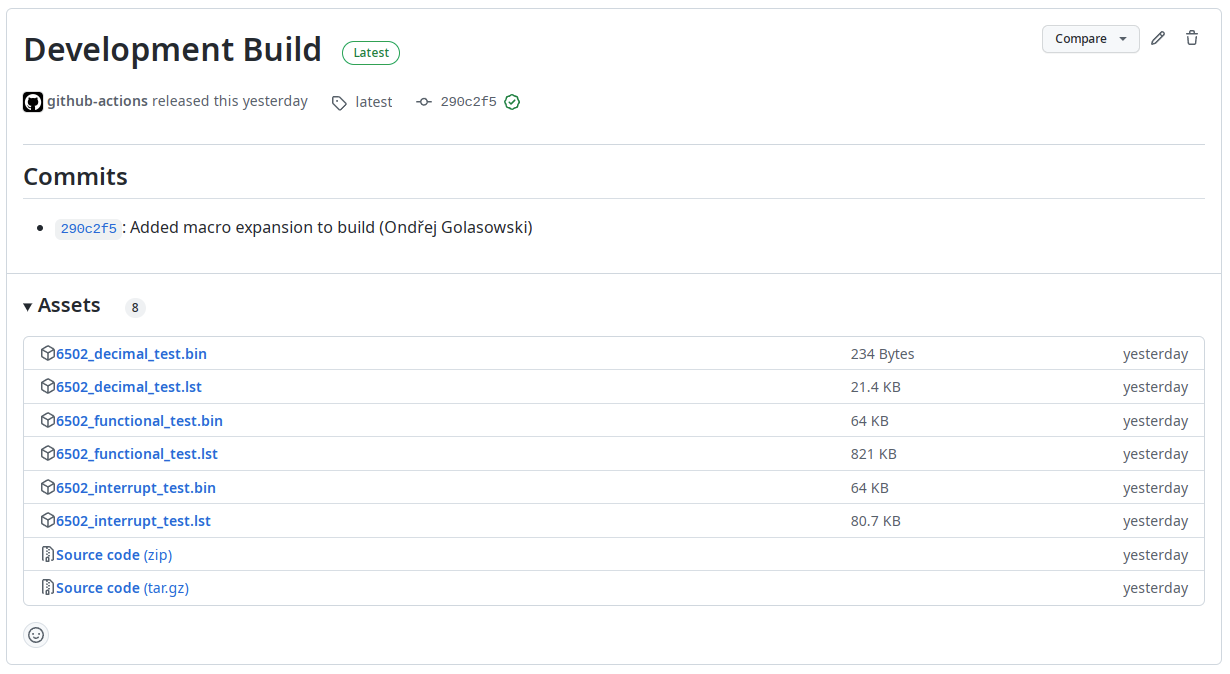
\includegraphics[width=0.8\textwidth]{images/vydani-testu-6502.png}
    \caption{Vydání testů pro procesor 6502.}
    \label{fig:vydani-testu-6502}
\end{figure}

\subsubsection{Integrace s Google Test}
Nakonfigurované a sestavené testy je nyní možné spouštět ručně. Pro automatické spouštění je nutné vytvořit testovací funkci pro platformu Google Test. Aby byly dodržovány zásady dobrého testování, je vhodné test vytvořit za použití existující komponenty, do které se nebudou přidávat žádné funkcionality pouze pro běh testu. Případné změny lze totiž provést přímo v~testu a~to za použití dědičnosti. Ve výpisu~\ref{list:6502-test-uprava} je znázorněna upravená třída procesoru. Je použit název DUT (Design Under Test), který se používá například při tvorbě testů ve VHDL. Důležitou úpravou je přidání rozhraní pro úpravu programového čítače, což je nutné pro spuštění testu a~kontroly stavu testu.

\begin{listing}[htp!]
	\caption{Upravený procesor 6502 v Google Test.}
	\label{list:6502-test-uprava}
	\begin{minted}{c++}
class DUT : public MOS6502 {
public:
	void step() {
		while(!instrFinished()) {
			CLK();
		}
		
		CLK();
	}
	uint16_t getPC() {
		return m_registers.pc;
	}

	void setPC(uint16_t val) {
		m_registers.pc = val;
	}

	void triggerNMI() {
		NMI();
	}

	void setIRQ(bool active) {
		IRQ(active);
	}
};
	\end{minted}
\end{listing}

Samotný test pak probíhá v~jednoduchém cyklu, kde podmínkou pro opuštění je opakovaná hodnota programového čítače. Ověření výsledku probíhá porovnáním poslední hodnoty programového čítače. Dle listingu vygenerovaného assemblerem lze zjistit, že úspěch je signalizován zacyklením na adrese \mintinline{text}|$06e5|, což ukazuje výňatek ve výpisu~\ref{fig:6502-test-uspech}. Celý testovací cyklus s~ověřením výsledku se nachází ve výpisu~\ref{list:6502-test-cyklus}.

\begin{listing}[ht!]
	\caption{Řádek signalizující úspěch v listingu testu 6502.}
	\label{fig:6502-test-uspech}
	\begin{minted}{ca65}
                                success         ; Navesti makra uspechu.
06e5 : 4ce506          >        jmp *           ; Test byl dokoncen uspesne.
	\end{minted}
\end{listing}

\begin{listing}[ht!]
	\caption{Testovací cyklus procesoru 6502 v Google Test.}
	\label{list:6502-test-cyklus}
	\begin{minted}{c++}
do {
	prevPC = cpu.getPC();
	cpu.step();
} while(prevPC != cpu.getPC());

EXPECT_EQ(prevPC, ADR_SUCCESS) 
	<< "The test failed on trap at address 0x"
	<< std::hex << prevPC;
	\end{minted}
\end{listing}


\subsubsection{Příklad testování}
Jedním z~problému, které se v~průběhu vývoje objevily, byl problém s~časováním přerušení. Byla proto vytvořena verze, která lépe odpovídá skutečnému chování. Kvůli tomu ale přestal fungovat test přerušení: \mintinline{text}|6502_interrupt_test.bin|. Tato část popisuje, jak se dá podobná chyba diagnostikovat a~opravit.

Test se zastavil na adrese \mintinline{text}|$6b2|. Dle listingu tato adresa odpovídá sekci, kde se testují obě přerušení, NMI a~IRQ. Část způsobující chybu je vyobrazena ve výpisu~\ref{list:6502-test-hledani-chyby}. Nejprve se nastaví vyvolání obou typů přerušení instrukcí \mintinline{text}|sta I_port|, přičemž IRQ bylo maskováno (pro stručnost není proces maskování uveden). Čeká se na provedení obslužné rutiny NMI a~otestuje se, zdali proběhlo. Poté se povolí přerušení IRQ instrukcí \mintinline{text}|cli|. Nyní by měla proběhnout rutina IRQ, k~tomu však nedojde a~test se zastaví.

\begin{listing}[htp!]
	\caption{Výňatek z~kódu testu signalizující chybu.}
	\label{list:6502-test-hledani-chyby}
	\begin{minted}{ca65}
; Testovani IRQ a NMI s maskovanim preruseni.
; ...
												; Testovani NMI
0699 : 8dfcbf          >        sta I_port      ; Vyvolani preruseni.

069c : e8                       inx
069d : e8                       inx
069e : e8                       inx
069f : ad0302                   lda I_src       ; Probehlo preruseni?
                                trap_ne
06a2 : d0fe            >        bne *           ; Pokud ne, skonci test.

06a4 : a200                     ldx #0

06a6 : a902                     lda #2          ; Testovani IRQ
06a8 : 8d0302                   sta I_src
06ab : 58                       cli             ; Povoleni IRQ.
06ac : e8                       inx
06ad : e8                       inx
06ae : e8                       inx
06af : ad0302                   lda I_src       ; Probehlo preruseni?
                                trap_ne
06b2 : d0fe            >        bne *           ; Pokud ne, skonci test.
	\end{minted}
\end{listing}

Již na základě této množiny informací lze chybu nalézt. Test nastaví zpětnovazební registr tak, aby byla vyvolána obě přerušení již při prvním testu, kdy se ověřuje NMI. V~dalším testu (ověření IRQ) již pouze povolí přerušení a~hodnotu ve zpětnovazebním registru nemění.

Skutečný procesor 6502 každé přerušení detekuje jiným způsobem. Přerušení IRQ detekuje úrovňový detektor. Při logické nule se zaznamená požadavek na přerušení a~po dokončení stávající instrukce se ověří, zdali přerušení není maskováno. Pokud je, provede se další instrukce normálním způsobem a~požadavek se zahodí. Tento požadavek je ale znovu zaznamenán, pokud je signál stále aktivní (tedy na logické nule). Emulovaný procesor vyvolal při zápisu do zpětnovazebního registru pouze jeden požadavek, choval se tedy jako hranový detektor, což je v~rozporu se skutečným procesorem, a~proto toto chování test vyhodnotil jako chybné. Hranový detektor je použit pouze u~NMI.

Stačí tedy funkci odpovídající pinu IRQ implementovat tak, aby se dal nastavovat jeho stav (aktivní a neaktivní), nikoliv pouze vyvolávat signál, jako je to u~NMI. Klíčovou část kódu ukazuje výpis~\ref{list:6502-preruseni-irq-oprava}.

\begin{listing}[ht!]
	\caption{Oprava chybné implementace IRQ.}
	\label{list:6502-preruseni-irq-oprava}
	\begin{minted}{c++}
void MOS6502::IRQ(bool active){
	m_irq = active;
}
	\end{minted}
\end{listing}


\begin{note}[Funkčnost původní implementace]
A proč tedy původní implementace fungovala? To bylo způsobeno jinou chybou, kdy se požadavek na přerušení ukládal, pokud bylo přerušení maskováno. To ale také neodpovídá skutečnému procesoru.
\end{note}

\subsection{Testování grafického čipu}
Čip 2C02 je nejkomplexnějším čipem celé konzole, byl testován v~několika fázích, především implementováním různých funkcionalit pro zobrazování obsahů paměti a~porovnávání s~popisem fungování zjištěným v~analytické části.

Jako první bylo nutné ověřit, jestli je správně mapován obsah grafické paměti. Pro tyto účely byly vytvořeny funkce, které renderují obsah pattern table s~možností přepínat paletu, která je použita. Takto byla odhalena i~první chyba, která překvapivě nebyla způsobena chybným přístupem do pattern table, ale špatně implementovanou pamětí palet. Nemá-li totiž program zajištěný korektní přístup do této paměti, zůstane paměť prázdná, a~tudíž i~pattern table bude vykreslena jako jednolitý čtverec. Po opravě chyb následuje ověření, že je obsah pattern table správně vykreslován. To je možné porovnáním s~funkčními emulátory, které obsahují debugger, popřípadě existují i~vyobrazení pattern table v~různých diskusích a~článcích.

Dalším krokem byla implementace zobrazování videopaměti. U~jednoduchých her jako \enquote{Donkey Kong}, které nepoužívají zrcadlení, stačí vykreslit první polovinu paměti tak, jak je uložena --- není potřeba pečlivě provádět sekvenci kroků popisovanou v~části~\ref{sec:ppu-pozadi}. To, jestli je obsah paměti správně vykreslen, lze velice jednoduše ověřit opět několika způsoby: spuštěním softwaru na jiném emulátoru, na skutečné konzoli, nebo prostým porovnáním screenshotů z~fór a~diskusí (což je však nejméně věrohodný zdroj).

Podobným způsobem byla vždy implementována další funkcionalita a~byla testována a~opravována tak dlouho, dokud nebyla funkční. Po implementaci všech základních funkcí čipu je možné zkoušet spouštět různé hry a~zjišťovat, zdali se chovají dle očekávání. Zde však existuje riziko, že samotná hra obsahuje neočekávané chování; některé hry například chybným přístupem do paměti způsobily poškození obrazu, popřípadě zobrazení nesmyslných textů. Například hra \enquote{Ghostbusters} načítá závěrečný text ze špatné pattern table, tudíž dojde k~zobrazení prázdné obrazovky.~\cite{Nesdev:game-bugs} Je jasné, že cílem softwarové emulace je především to, aby správně běželo původní programové vybavení, tudíž testování spouštěním tohoto softwaru je validní. Ovšem důkladnější ladění je možné jen při použití softwaru, jehož chování je přesně definováno. Takovou roli zastávají testy vytvořené komunitou, která vyvinula testovací programy, definovala jejich chování na reálném systému a~zveřejnila je. Velká část používaných testů pochází z~Nesdev~\cite{Nesdev:tests}.

\subsection{APU}
Komponentu APU je složité testovat automatizovanými testy, jelikož je zvukový výstup ovlivněn vlastnostmi použitého filtru. Ruční testy lze provádět pomocí nahrávání zvukového výstupu aplikace a~analýzy výsledného průběhu signálu. Nástroj, který lze pro tyto účely použít, je Audacity.

V~průběhu vývoje APU byl zjištěn problém s~výstupem zvuku. Generovaný zvuk obsahoval nepříjemné praskání.

První krokem bylo zjistit, který kanál je zdrojem problému, tudíž z~výsledného mixu nejprve odstranit pulzní kanál jeho jednoduchým odstraněním z~mixovacího výpočtu a~ponecháním pouze pulzního kanálu. Bylo nutné vybrat software, který určitě používá kanál pro generování šumu; takovým je například hra \enquote{Super Mario Bros.}. Po spuštění softwaru šlo stále slyšet praskání; problémový kanál tak byl identifikován. Nyní je možné nahrát výstup aplikace a~podrobně prozkoumat průběh výstupního signálu. Průběh vyobrazený aplikací Audacity je znázorněn na obrázku~\ref{fig:test-sum-chybne}.

\begin{figure}[ht!]
	\centering
	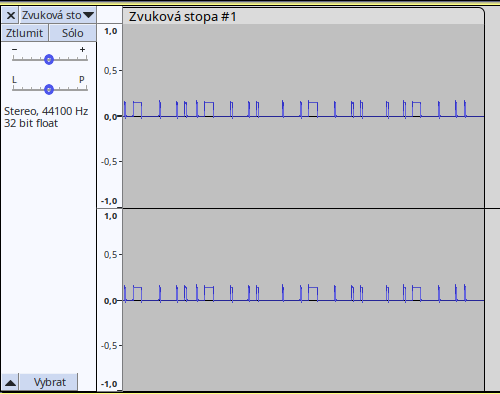
\includegraphics[width=0.5\textwidth]{images/audacity_chybne.png}
	\caption{Ukázka chybného výstupu generátoru šumu.}
	\label{fig:test-sum-chybne}
\end{figure}

Lze vidět, že zjištěný průběh zdaleka nepřipomíná šum. Ze znalosti principu fungování generátoru šumu lze usoudit, že problém může být způsoben posuvným registrem; je totiž komponentou, která rozhoduje, zdali bude na výstup puštěna hodnota obálky signálu.

Nejprve bylo zkontrolováno, jestli byla správně implementována zpětná vazba, což se potvrdilo. Dále bylo zkontrolováno, zdali dochází ke korektní inicializaci. Chyba byla právě zde; registr byl inicializován na hodnotu 0, přitom dle \cite{Nesdev:apu-noise}: \enquote{On power-up, the shift register is loaded with the value 1.}

Opravením výchozí hodnoty na 1 byl problém vyřešen. Výstup již zněl tak, jako zní ze skutečné konzole či jiných emulátorů.

\subsection{Další komponenty}
Testování dalších komponent probíhalo obdobně, jako bylo již popsáno výše. Herní ovladače byly otestovány reakcemi softwaru, takto byla například objevena chyba v~implementaci posuvných registrů zmíněná v~sekci~\ref{sec:impl-dalsi}, kdy se hra \enquote{Super Mario Bros.} spoléhala na jistou hodnotu po přečtení celého registru.

Kazeta a~mappery poté byly testovány automaticky pomocí testů na platformě Google Test, stejně jako společné komponenty. Velice důkladně bylo otestováno fungování přepínání bank, protože i~malá chyba může způsobit, že se kód začne číst z~jiné adresy a~celý program přestane fungovat, stejně závažná je i~chybná implementace zrcadlení videopaměti, což v~případě tohoto projektu také zajišťuje kazeta, tudíž je zrcadlící funkcionalita také testována v~rámci těchto testů.

\section{Shrnutí}
Jak je zřejmé z~předchozích odstavců, bez průběžného testování by nebylo možné emulátor vyvinout. I~přes to však zbývá mnoho prostoru pro vylepšení testů, především pro zvukový a~grafický čip. Pro grafický čip je možné testy provádět tak, že se pořídí snímek obrazovky, vytvoří se kontrolní součet a~ten se porovná se \enquote{zlatým standardem}, neboli s~výstupem emulátoru, který je určitě implementován správně. Takové testy budou užitečné především pro budoucí implementátory emulátorů, kteří by si chtěli jednoduše vyzkoušet, jestli je jejich emulátor správně fungující.

%---------------------------------------------------------------
\chapter{Navazující práce}
%---------------------------------------------------------------
Bakalářská práce otevřela mnoho témat, se kterými lze dále pracovat a~na které lze navázat další prací, což stručně popisuje tato kapitola. Navazovat lze nejen na vývoj emulátoru NES, ale i~emulační platformy, popřípadě lze emulační platformu využít pro vývoj jiných emulátorů.

\section{Rozšíření emulátoru konzole}
Emulovaná konzole NES v~projektu sice již obsahuje vše, co je potřeba pro spouštění jednodušších i~složitějších her, avšak vzhledem ke komplexitě systému je mnoho prostoru pro rozšíření a~zvýšení věrohodnosti emulace.

Přímočaře lze rozšířit množství emulovaných mapperů. Tím, že pro NES vzniklo mnoho softwaru, vzniklo spoustu mapperů použitých třeba~jen v~jednotkách kazet. Mnoho mapperů vzniklo i~pro podporu kazet s~více hrami (takzvané multicarts).

Dále lze jednoznačně rozšířit počet emulovaných zvukových kanálu čipu APU. Ještě zbývá implementovat emulaci generátoru trojúhelníkového signálu a~kanálu pro přehrávání surových zvukových dat.

Hotové emulované součásti NES je také možné ještě vylepšit, například lze implementovat další hardwarové specifika grafického čipu, aby bylo možné spouštět hry simulující trojrozměrný prostor (například \enquote{Ferrari Grand Prix Challenge}).

\section{Rozšíření emulační platformy}
Dalším výsledkem práce je emulační platforma Universal~System~Emulator. Platforma je zveřejněna v~repozitáři na~GitHubu~\cite{Golasowski2023:use}. Rozšiřování projektu se dá rozdělit do dvou různých částí: rozšíření platformy a~rozšiřování balíku podporovaných komponent a~systémů.

\subsection{Rozšíření funkcionality}
Samotná platforma má několik chybějících funkcionalit, které jsou využitelné napříč různými emulátory, například zaznamenávání historie stavu komponent a~jeho ukládání. Další funkcionality vhodné k~implementaci se týkají především přenositelnosti emulátoru: zajištění správného fungování zvuku na všech platformách a~nastavení automatické kompilace pro webové prohlížeče (WebAssembly, nástroj Emscripten).

Rozsáhlým plánovaným rozšířením je grafický editor systémů. Rozhraní komponenty bylo již v~rámci bakalářské práce navrhováno tak, aby bylo možné do platformy přidat způsob, jakým s~komponentami pracovat v~grafickém editoru a~skládat je takto do funkčního systému. Tím, že platforma nabízí možnosti komunikace mezi komponentami až na úrovni digitálních signálů, nabízí se mnoho různých zajímavých využití potenciálního grafického editoru. Implementují-li se do platformy hradla, bude možné sestavovat logické obvody. Samozřejmě bude možné propojovat i~stávající komponenty, do obvodu bude tedy jednoduché zapojit například i~procesor 6502. 

Bude-li implementován grafický editor, bude vhodné prozkoumat další využití tohoto editoru ve výuce. Jedním z~návrhů je implementace komponent potřebných k~sestavení mikroarchitektury založené na RISC-V ISA. Takto by bylo možné RISC-V kompatibilní procesor sestavit graficky a~sledovat průběhy signálů mezi jednotlivými komponentami, což bude zajímavé především pro účely výuky počítačových architektur. V~rámci dodatečné rešerše bylo zjištěno, že existují projekty schopné překládat komponenty popsané v~jazyce Verilog do jazyka C/C++ (například \emph{v2c} a~\emph{Verilator}). Vytvořilo-li by se rozhraní mezi existujícími metodami propojení komponent a~rozhraním generovaným těmito nástroji, bude možné do platformy přímo importovat komponenty popsané v~jazyce pro popis hardwaru.

S~výše uvedeným editorem systémů také souvisí možnost vytvářet a~upravovat kód v~jazyce symbolických adres, který by byl na systémech spouštěn. Díky tomu bude moct uživatel napsat kód, který se přeloží do spustitelného strojového kódu přímo na emulované komponentě, kde uživatel uvidí, jak dochází ke zpracování jím napsaného programu.

\subsection{Implementace komponent}
Tím, že je platforma navržena univerzálně, lze libovolně přidávat další emulované komponenty. Mezi navrženými komponentami, které by byly zajímavé na implementaci, je například jednoduchý $16 \times 2$ LCD displej mapovaný do paměti. Tento displej by bylo možné připojit například k~procesoru, který by na displej mohl vypisovat přímo z~programu.

Dalším návrhem je implementace procesoru CHIP-8, což je jednoduchý procesor obsahující i~primitivní způsob vykreslování grafiky. Je možné implementovat i například~koncept procesoru URISC (ultimate reduced instruction set computer, procesor s~ISA obsahující jedinou instrukci), což je užitečné jako demonstrace primitivního, ale univerzálního počítače.

\section{Vývoj dalších emulátorů}
Emulační platforma je vhodná jako základ pro využití dalšími projekty, které mají za cíl vytvořit celý emulátor nějakého systému. Díky projektu tito vývojáři nebudou muset přemýšlet, jak vytvořit grafický debugger, jak implementovat zvuk, nebo pro jakou platformu vyvíjet. Platforma Universal System Emulator totiž vše zmíněné zařizuje sama a~navíc je plánována podpora všech hlavních operačních systémů --- Linux, Windows, macOS, Android a~všechny ostatní, na kterých běží moderní webový prohlížeč (Firefox, Safari a~prohlížeče založené na projektu Chromium).

Vývojář emulátoru se tak bude již od začátku vývoje emulátoru zabývat pouze vývojem jednotlivých komponent a~jejich propojování do fungujícího systému, což ušetří mnoho času a~umožní vývojáři se soustředit na části vývoje spjaté s~hardwarem.

Aby se vývoj emulátorů co nejvíce ulehčil, byla vytvořena podrobná dokumentace obsahující popis rozhraní generovaný z~komentářů v~kódu emulátoru a~také podrobný návod k~vývoje vlastních komponent a~systému. Tuto dokumentaci si mohou vývojáři buďto vygenerovat sami pomocí návodu v~repozitáři~\cite{Golasowski2023:use}, nebo mohou využít průběžně automaticky generovanou dokumentaci na GitHub~Pages, na níž je odkazováno také v~repozitáři projektu~\cite{Golasowski2023:use}.

Emulační platformu Universal System Emulator nemusí využít jenom hobby programátoři, kteří se chtějí o~svém oblíbeném systému dozvědět více vývojem emulátoru, ale například i~studenti, kteří takto chtějí bádat v~rámci své závěrečné práce; ať už maturitní nebo bakalářské.

%---------------------------------------------------------------
\chapter*{Závěr}\addcontentsline{toc}{chapter}{Závěr}\markboth{Závěr}{Závěr}
%---------------------------------------------------------------
Primárním cílem práce bylo vytvořit funkční softwarový emulátor konzole Nintendo Entertainment System. Cíl zahrnoval využití ve výuce, což vyžadovalo vývoj přehledného grafického rozhraní. Primární cíl byl v~průběhu 2~let vývoje bakalářského projektu značně rozšířen o~cíle sekundární, kdy nejdůležitějším bylo vytvoření univerzální platformy pro vývoj emulátorů.

Pro dosažení primárního cíle byla nezbytná \emph{důkladná analýza}. Za pomocí hardwarových manuálů a~komunitní dokumentace byl vytvořen přehled principů stojících za fungováním jednotlivých komponent konzole NES. Výsledky analýzy byly popsány v~textu bakalářské práce, což z~textu vytvořilo užitečný přehled pro potenciální zájemce nejen o~vývoj vlastního emulátoru NES, ale i~o~pochopení principu fungování velmi rozšířené herní konzole. Podrobně bylo popsáno fungování procesoru 6502 včetně jeho varianty 2A03: zpracování instrukcí, práce s~pamětí i~obsluha přerušení. Byly vysvětlen způsob vykreslování grafiky čipem 2C02 i~principy jeho vnitřních procesů doplněných o~přehledné ilustrace --- od uchovávání grafických informací v~paměti přes vyhodnocení až po samotné zobrazení na obrazovce. Analyzovány a~popsány byly také kazety pro distribuci softwaru včetně obvodů pro mapování paměti. Jako poslední byly popsány periferie a~čip pro zpracování a~přehrávání zvuku. V~poslední podkapitole byla shrnuta existující řešení emulace konzole. 

Následovala \emph{návrhová část}. V~této části bylo na základě výsledků analýzy navrženo optimální řešení. Po výběru programovacího jazyka jakožto i~vhodných nástrojů pro vývoj, správu zdrojového kódu, dokumentace a~provádění testování byla navrhována platforma pro vývoj emulátoru. Návrh emulační platformy zabral značnou část vývojového procesu, musel být totiž navržen vhodný stupeň abstrakce i~způsob reprezentace komponent a~jejich propojení. Byly navrženy a~otestovány různé varianty platformy; všechny jsou popsány v~textu. Nakonec byla zvolena varianta univerzální platformy využitelné pro další emulační projekty, jelikož existuje mnoho zájemců o~tvorbu vlastního emulátoru. Samotná platforma je tak dobře použitelná pro vzdělávací účely, například jako základ maturitní i~bakalářské práce. Po navržení platformy již byla navržena implementace konkrétních komponent NES. Byly například vybírány vhodné způsoby dekódování operačních znaků ISA 6502, úroveň abstrakce emulace grafického čipu i~způsoby vytváření zvukových vzorků v~emulaci zvukového čipu. Tyto úvahy mohou vzhledem ke své obecné platnosti pomoci dalším vývojářům emulátorů.

Po analýze a~navržení následovala samotná \emph{implementace vybraného řešení}. Nejprve byly implementovány emulované komponenty NES na raných verzích emulační platformy. V~průběhu implementace byly řešeny různé problémy, které jsou popsané v~implementační části. Mezi takovými problémy byl například návrh záznamů dekódovací tabulky, rozdělení zodpovědností metodám v~implementace třídy emulující grafický čip nebo konkrétní implementace zvukového výstupu v~závislosti na platformě. Bylo totiž nutné vyřešit, zdali posílat surový zvukový výstup generátorů pulzů, nebo tento výstup aproximovat pomocí Fourierových řad. Později byla postupně vytvářena univerzální platforma, ze které vznikl projekt Universal~System~Emulator dostupný na GitHubu. Do tohoto projektu byly emulované komponenty plně integrovány, vznikl tak i~referenční systém projektu. V~rámci sekundárních cílů byl implementován doplněk grafické knihovny používané v~projektu. Tento doplněk přidává chybějící funkcionalitu mapování uživatelských vstupů na akce a~je k~dispozici jako open-source na platformě GitHub pod názvem ImInputBinder.

Důležitá část vývoje, \emph{testování}, probíhala průběžně. Byly vyzkoušeny různé varianty testování od ručního porovnávání výsledků s~reálným systémem až po plně automatizované testy. V~příslušné kapitole byly popsány i~zajímavé problémy, které testování odhalilo, a~způsoby řešení těchto problémů. Pro účely testování procesoru 6502 vznikl další vedlejší projekt, který zajistil automatické kompilace a~vydávání testů ve strojovém kódu tak, aby je bylo možné definovat jako závislost projektu v~nástroji CMake.

V~poslední kapitole byly popsány \emph{navazující práce}. Bakalářská práce otevřela různá témata, na které je možné navázat, což primárně spočívá v~dalším rozšíření emulace NES. Lze doplnit emulaci dalších obvodů pro mapování paměti, zvýšit věrohodnost emulace grafického čipu, doplnit emulované periferie\dots Dále se jedná o~využití emulační platformy nejen pro vývoj emulátorů, ale například i~pro výuku počítačových architektur pomocí demonstrace mikroarchitektur RISC-V přímo na platformě. Všechna další využití jsou podpořena podrobnou dokumentací, která je dostupná i~ve webové verzi.

Bakalářská práce tedy splnila primární cíl definovaný v~zadání. Emulátor NES je funkční, je schopen spouštět jednoduché i~složitější programy pro originální konzoli, obsahuje přehledné rozhraní a~byl otestován a~srovnán s~fungováním původního hardwaru. Primární cíle zadání byly doplněny o~množství sekundárních cílů majících za úkol přinést alternativní metody výuky počítačových architektur, které byly také splněny dle očekávání.